\documentclass{beamer}
\usetheme{focus}

\usepackage{amsmath}
\usepackage{braket}
\usepackage{listing}
\usepackage{verbatim}

\definecolor{main}{RGB}{170, 85, 0}
\definecolor{background}{RGB}{240, 247, 255}

\title{Implementazione di un algoritmo KNN multiclasse su hardware quantistico}
\subtitle{Tesi di laurea sperimentale in fisica}
\author{Mariano Mollo N85000880\texorpdfstring{\\}{,} Relatori: \texorpdfstring{\\}{,} Giovanni Acampora \texorpdfstring{\\}{,} Autilia Vitiello}
\titlegraphic{
\includegraphics[scale=0.15]{gfx/logo-federico-II-blu}}
\institute{Università degli Studi di Napoli Federico II\texorpdfstring{\\}{,} Scuola Politecnica e delle Scienze di Base}
\date{25 ottobre 2019}

% [x] Le icone sono sgranate, sostiuirle con versioni di qualità migliore. 
% [x] Mettere slide sulle porte quantistiche usate
% [x] Si può inserire un'altra slide in cui si scrive l'equazione del QDB. 
% [x] Quando si introducono i qubit, mettere una slide sui registri a qubit multipli. 
% [x] Mettere gli obiettivi appena dopo l'introduzione. 
% [x] Metti numeretti di classe nel grafico dei cluster
% [x] Suddividi graficamente le varie parti del circuito semplice

\begin{document}
    \begin{frame}
        \maketitle
    \end{frame}

    % \section{Introduzione}

    \begin{comment}
    \begin{frame}{Machine learning}
        \begin{columns}
            \column{.5\textwidth}
            \begin{center}
                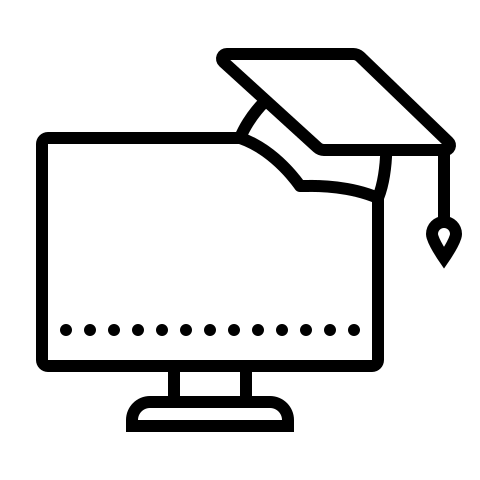
\includegraphics[width=.5\columnwidth]{gfx/icons/icons8-machine-learning-480}                
            \end{center}            

            Il machine learning è un ramo dell'intelligenza artificiale che permette ai computer di apprendere dai dati. 

            L'apprendimento può formalizzarsi attraverso la definizione di modelli matematici, usati per:
            \column{.5\textwidth}
            \begin{columns}
                \column{.5\textwidth}
                riconoscimento facciale e delle emozioni
                \column{.5\textwidth}
                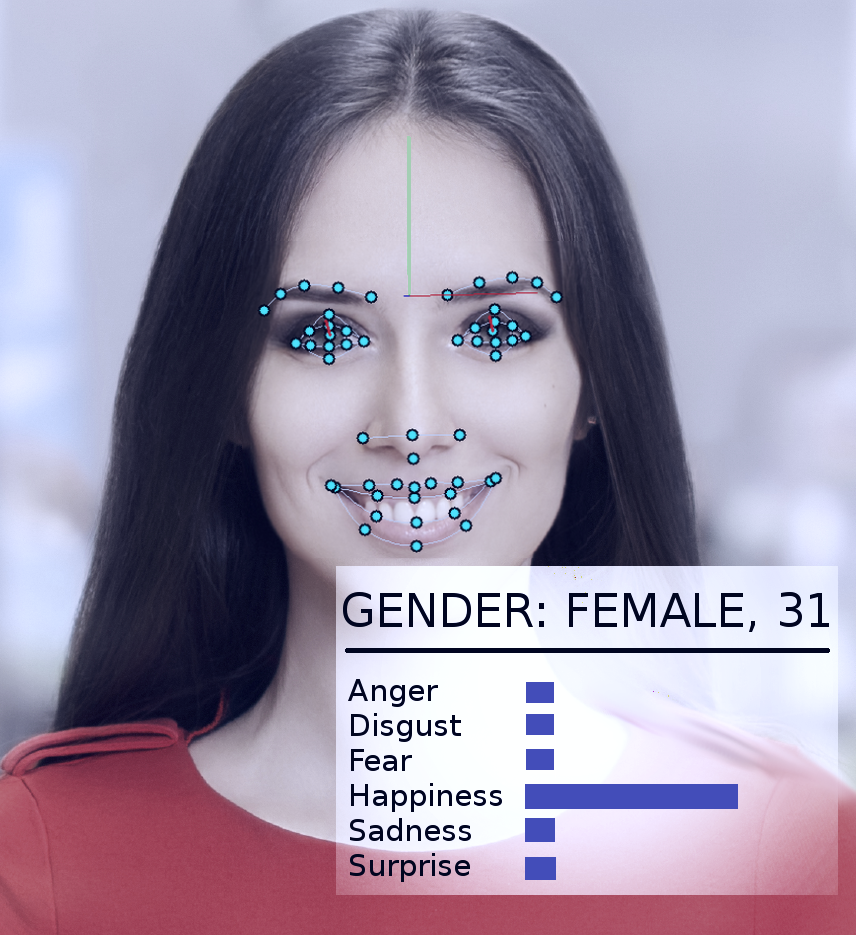
\includegraphics[width=\columnwidth]{gfx/Visage_Technologies_Face_Tracking_and_Analysis.png}
            \end{columns}

            \begin{columns}
                \column{.5\textwidth}
                veicoli a guida autonoma
                \column{.5\textwidth}
                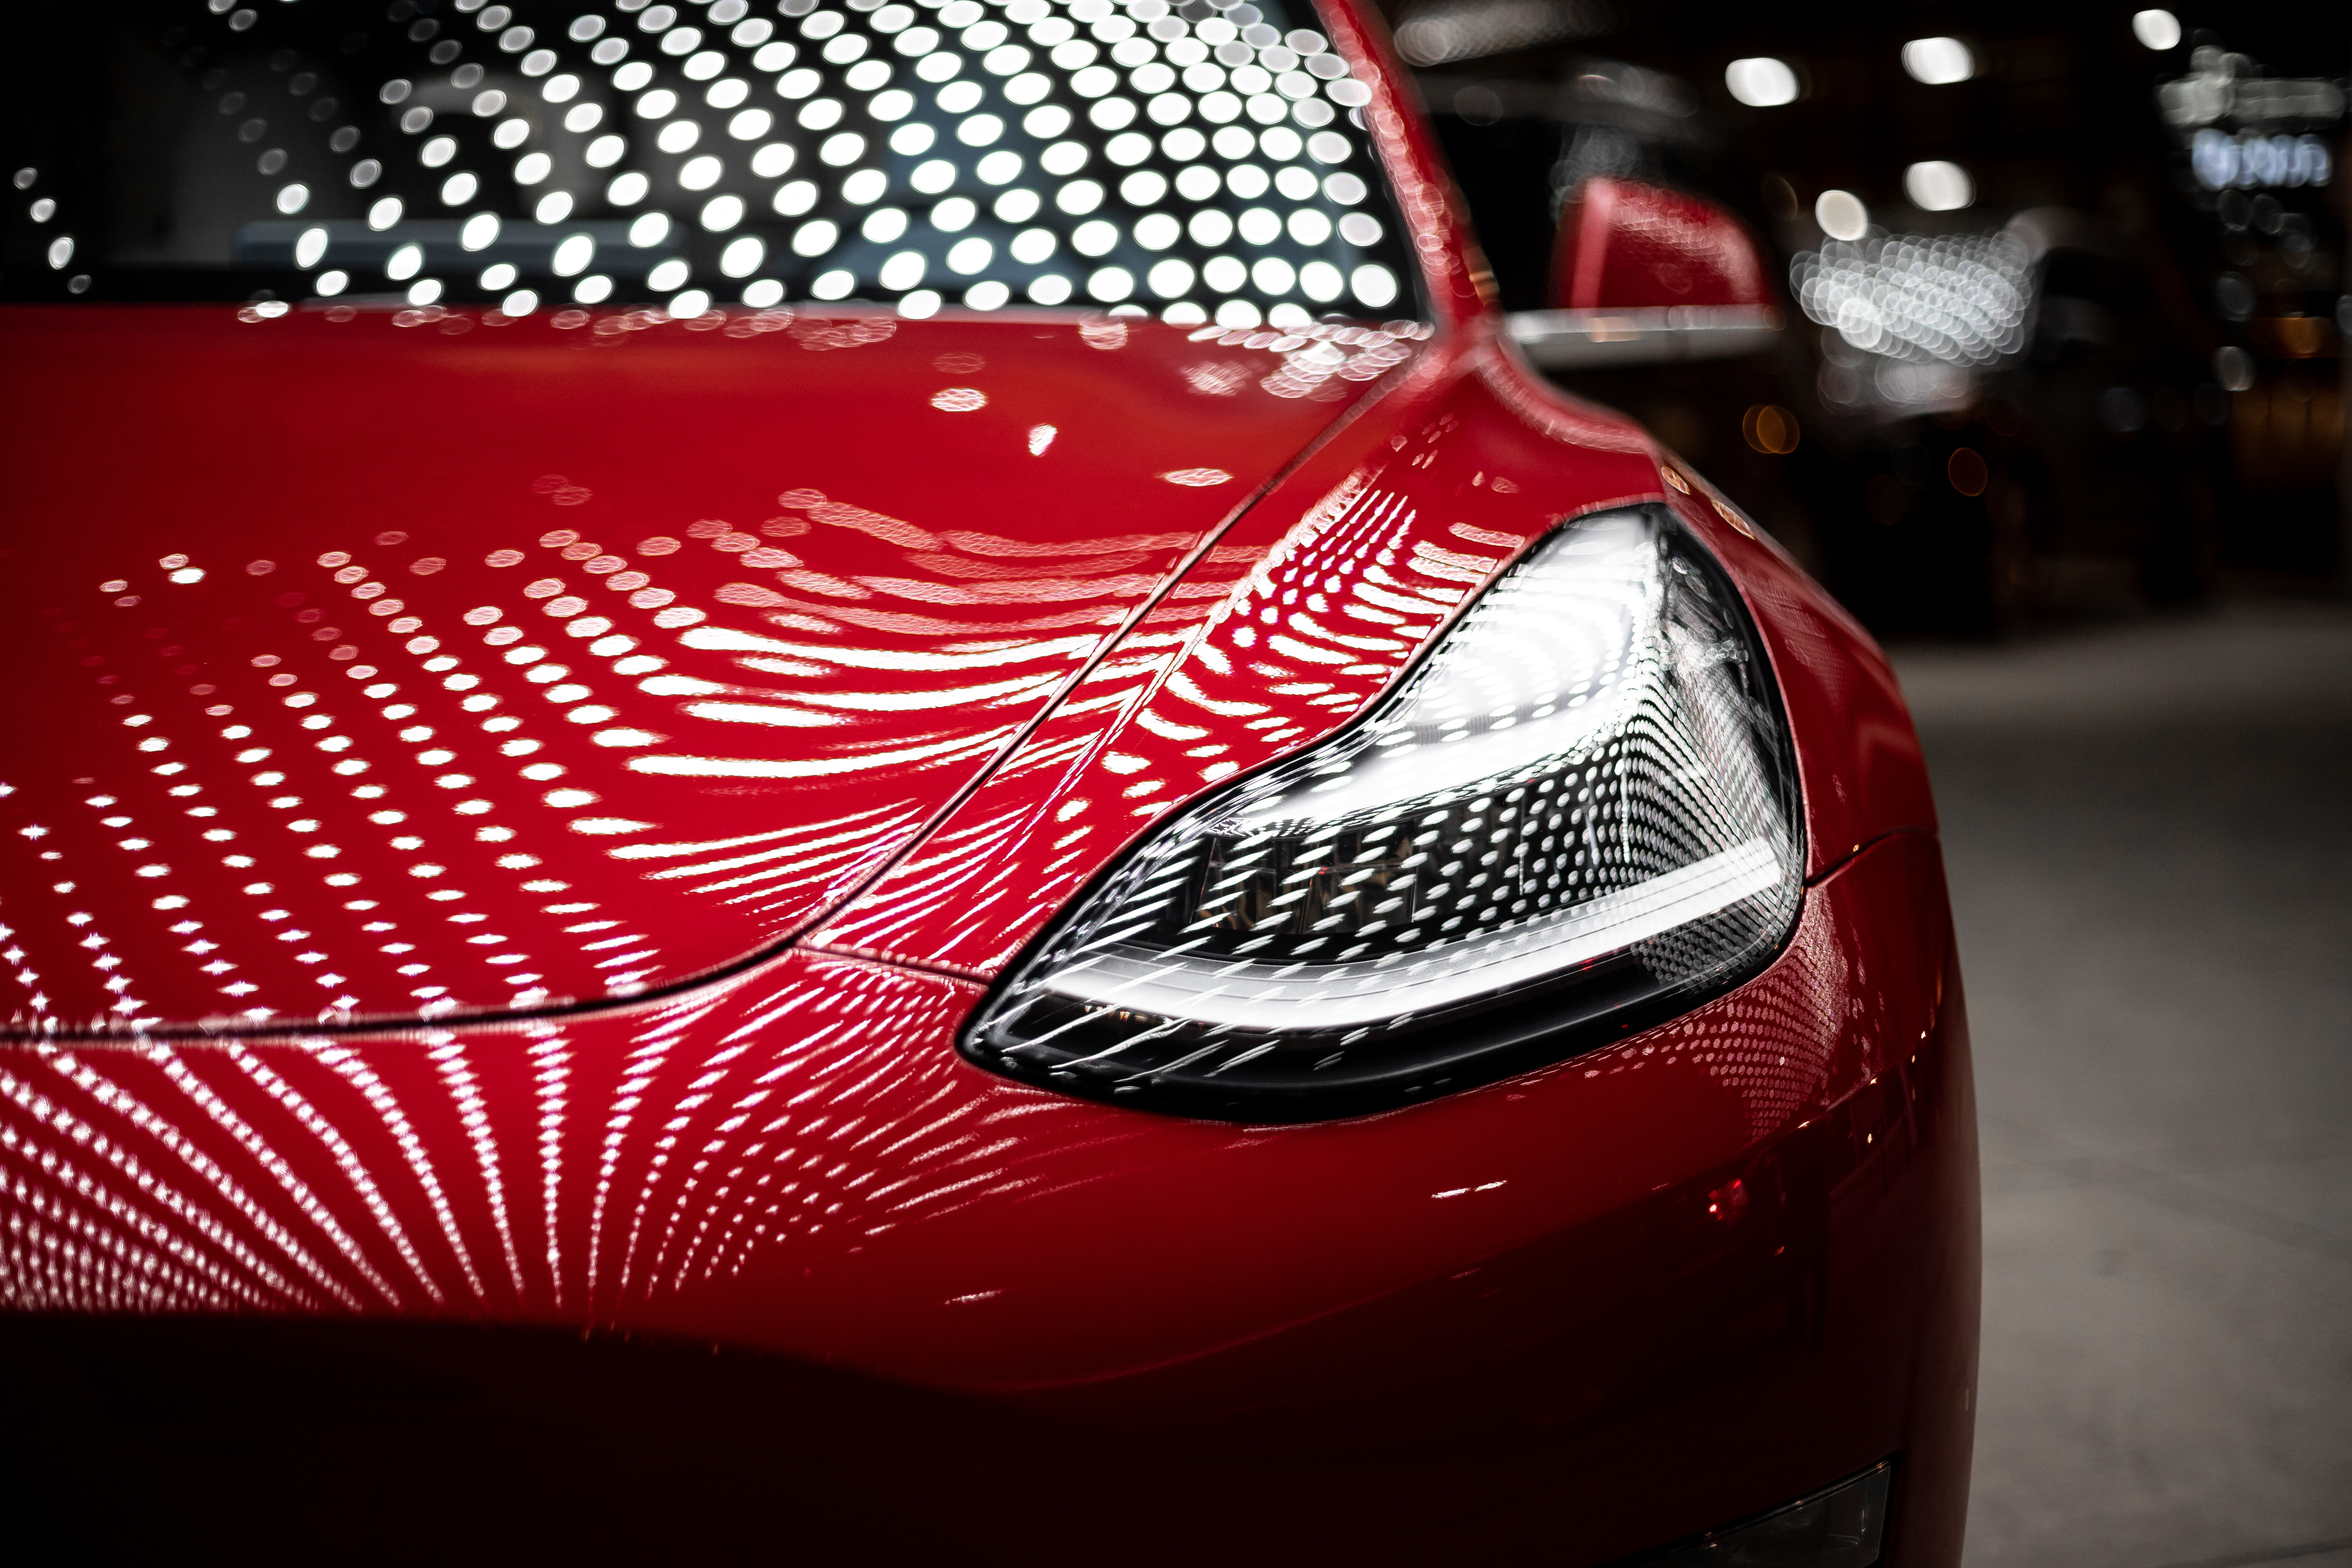
\includegraphics[width=\columnwidth]{gfx/tesla.jpg}
            \end{columns}

            \begin{columns}
                \column{.5\textwidth}
                identificazione dei sintomi di malattie
                \column{.5\textwidth}
                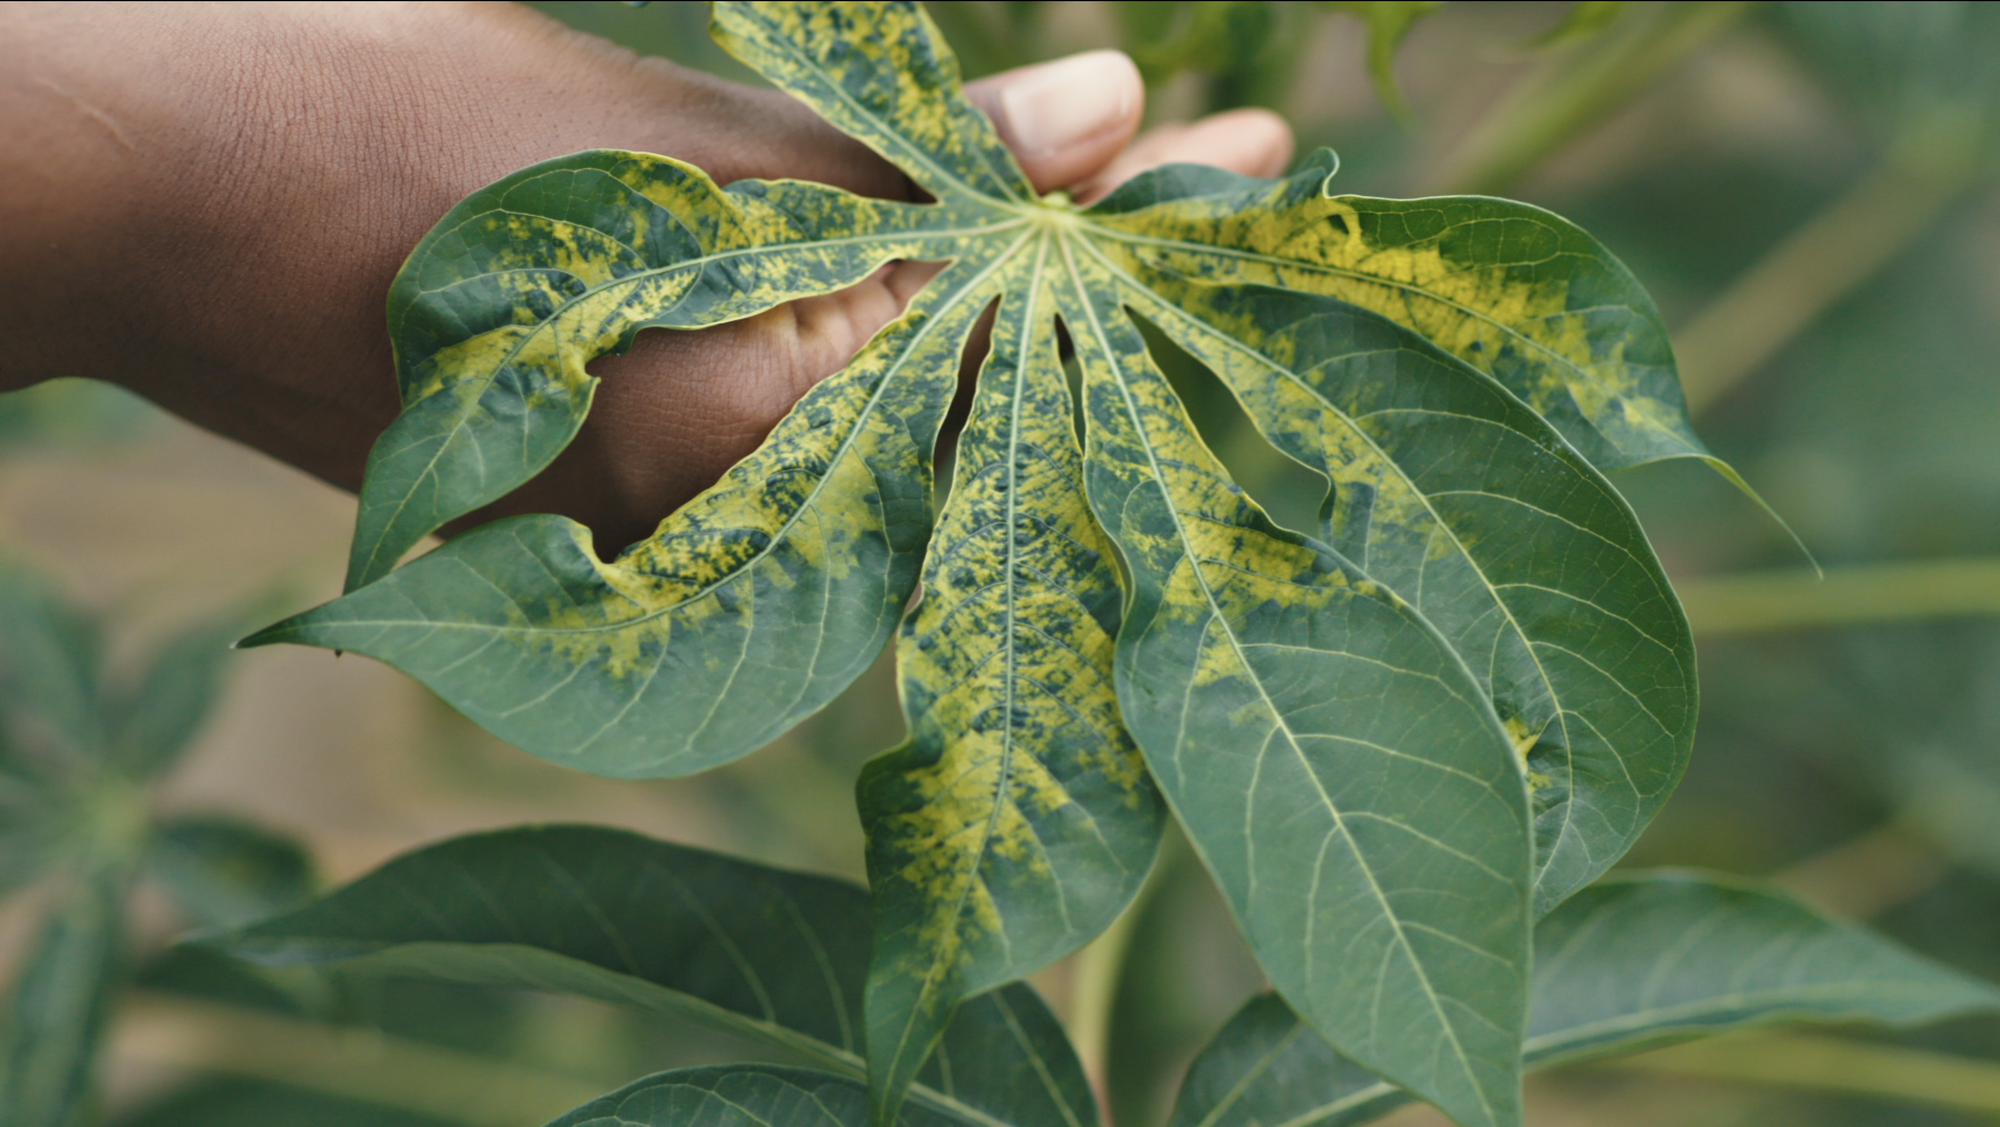
\includegraphics[width=\columnwidth]{gfx/pianta_malata.png}
            \end{columns}
        \end{columns}
    \end{frame}

    \begin{frame}{Quantum computing}
        \begin{columns}
            \column{0.5\textwidth}
            \begin{center}
                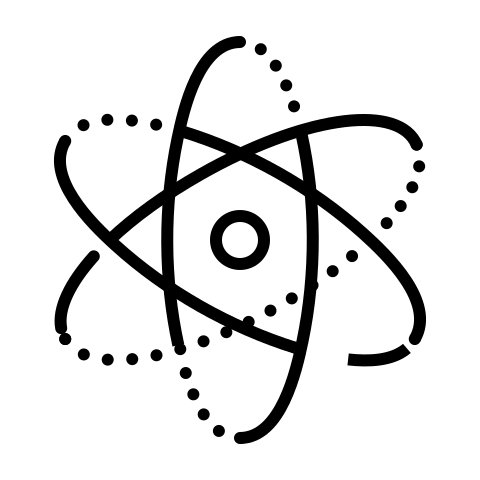
\includegraphics[width=.5\columnwidth]{gfx/icons/icons8-physics-480}                
            \end{center}
            
            Il quantum computing studia la costruzione e l'uso di hardware di elaborazione basato sulla meccanica quantistica
            \column{0.5\textwidth}
            \begin{itemize}
                \item Il quantum computing lavora con vettori in spazi di Hilbert complessi
                \item I computer quantistici eseguono operazioni lineari sui qubit
                \item Sistemi a molti qubit sono descritti da grandi vettori che possono essere manipolati in parallelo
            \end{itemize}
        \end{columns}
    \end{frame}

    \begin{frame}{Quantum machine learning}
        \begin{columns}
            \column{0.3\textwidth}
            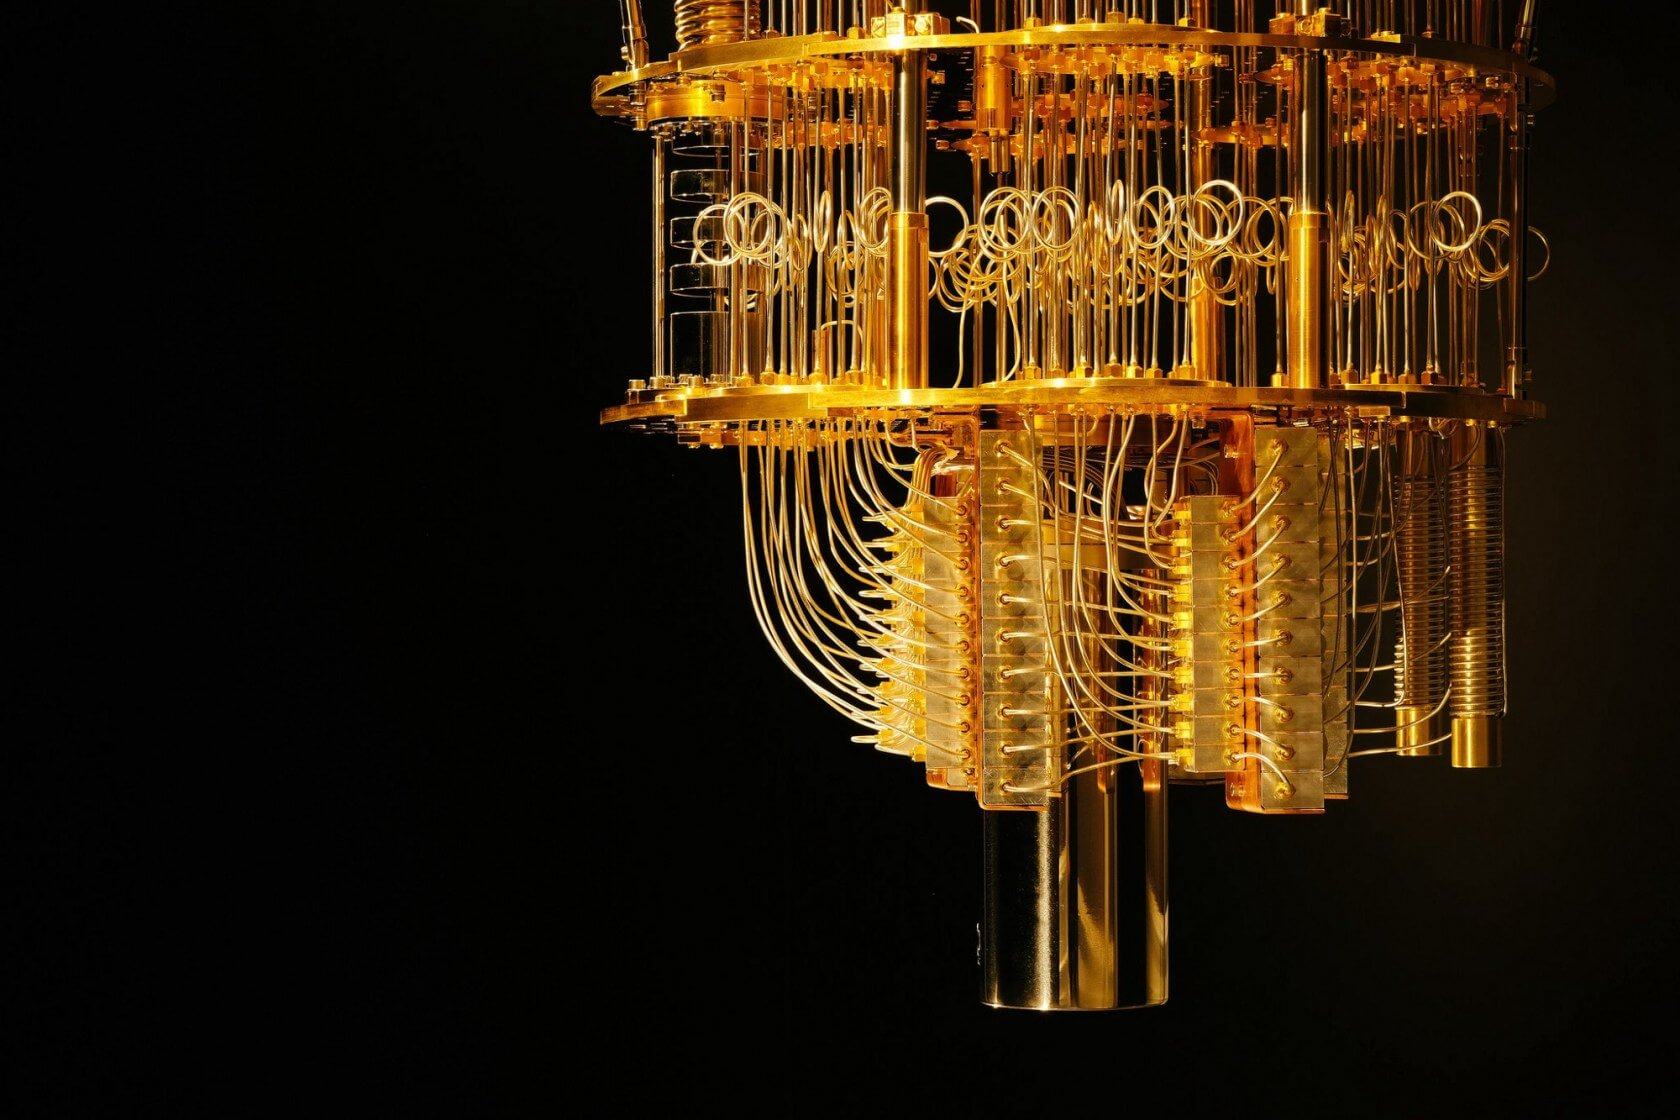
\includegraphics[width=\textwidth]{gfx/quantum-computer.jpg}
            \column{0.7\textwidth}
            Il machine learning prevede la manipolazione di grandi vettori e matrici.

            \vspace{1cm}

            L'uso dei computer quantistici per risolvere problemi classici difficili o classi di problemi completamente nuove è chiamato machine learning quantistico, 
            ovvero il permettere ai computer quantistici di imparare dai dati più velocemente dei computer classici
        \end{columns}
    \end{frame}
    \end{comment}

    \begin{frame}{Quantum machine learning}
        \begin{columns}
            \column{.33\linewidth}
            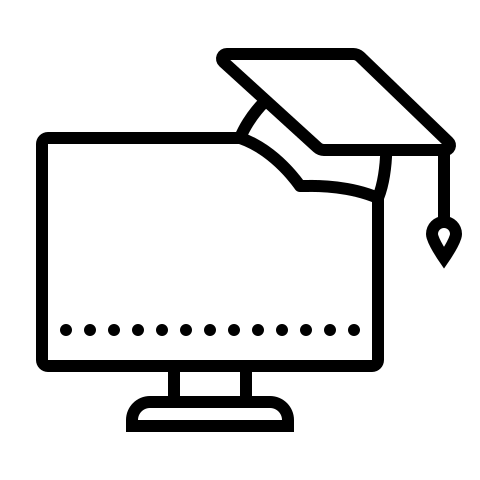
\includegraphics[width=\columnwidth]{gfx/icons/icons8-machine-learning-480.png}
            \begin{center}
                ML
            \end{center}
            permette ai computer di apprendere dai dati: riconoscimento facciale, guida autonoma, etc.
            \column{.33\linewidth}
            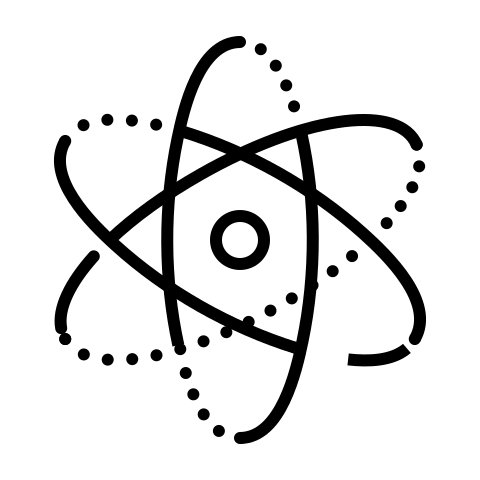
\includegraphics[width=\columnwidth]{gfx/icons/icons8-physics-480.png}
            \begin{center}
                QC
            \end{center}
            impiega la meccanica quantistica per eseguire calcoli più velocemente ed in maniera inaccessibile ai computer classici
            \column{.33\linewidth}
            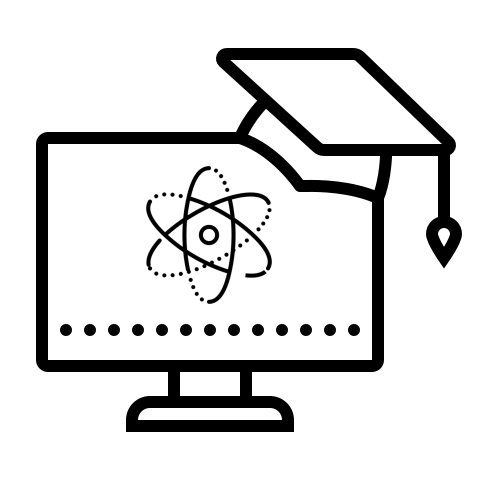
\includegraphics[width=\columnwidth]{gfx/icons/quantum-machine-learning-480.png}
            \begin{center}
                QML
            \end{center}
            risolvere problemi difficili e sconosciuti impiegando la meccanica quantistica
        \end{columns}
    \end{frame}

    \begin{frame}{Obiettivo di ricerca}
        È possibile implementare su un computer quantistico un 
        algoritmo k-nearest neighbours multiclasse, in modo da 
        migliorare le prestazioni ed il numero di problemi risolvibili? 

        \vspace{.5cm}

        Passaggi: 
        \begin{itemize}
            \item Riprodurre l'algoritmo di classificazione KNN quantistico a due classi proposto da Schuld et al. \cite{schuld} e implementarne una versione multiclasse su processore quantistico dell'IBM
            \item Analizzare le capacità dell'algoritmo attraverso esecuzioni su hardware quantistico e tramite simulazione
        \end{itemize}
    \end{frame}

    \iffalse
    \begin{frame}{Machine learning supervisionato}
        \begin{block}{Definizione del problema}
            Dato un insieme dati in input con i corrispondenti output, predire l'output di un nuovo input ignoto. 
        \end{block}

        \vspace{.5cm}

        \begin{columns}
            \column{.7\textwidth}
            Esempio: \emph{riconoscimento di caratteri scritti a mano}. 
            
            \vspace{.5cm}

            L'insieme dati di addestramento è 
            formato da molteplici caratteri scritti a mano per ciascun numero o 
            lettera dell'alfabeto. 

            \column{.3\textwidth}
            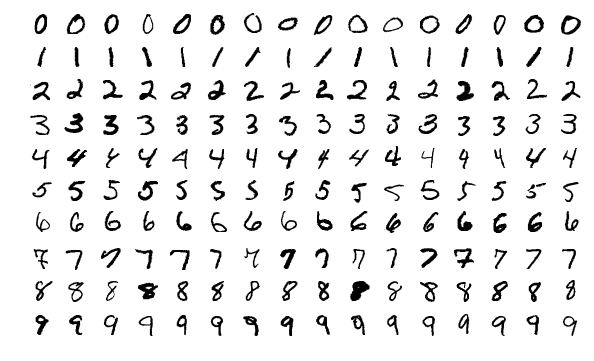
\includegraphics[width=\columnwidth]{gfx/MnistExamples}
        \end{columns}
        
        % \begin{tabular}{cc}
        %     Input & Output \\ \hline
        %     facce & emozioni \\ 
        %     battito cardiaco & stato di salute \\ 
        %     meteo dell'anno scorso & meteo di domani \\ 
        %     messaggio di un utente & intenzione del messaggio \\ 
        %     cronologia di ricerca & probabilità di cliccare su un annuncio
        % \end{tabular}
    \end{frame}
    \fi

    \begin{frame}{k-nearest neighbours classico pesato}
        \begin{columns}
            \column{0.4\textwidth}
            L'algoritmo di classificazione KNN è uno tra i più semplici del ML ed è un lazy learner

            \vspace{.5cm}

            Sia $k$ un numero naturale 

            \begin{center}
                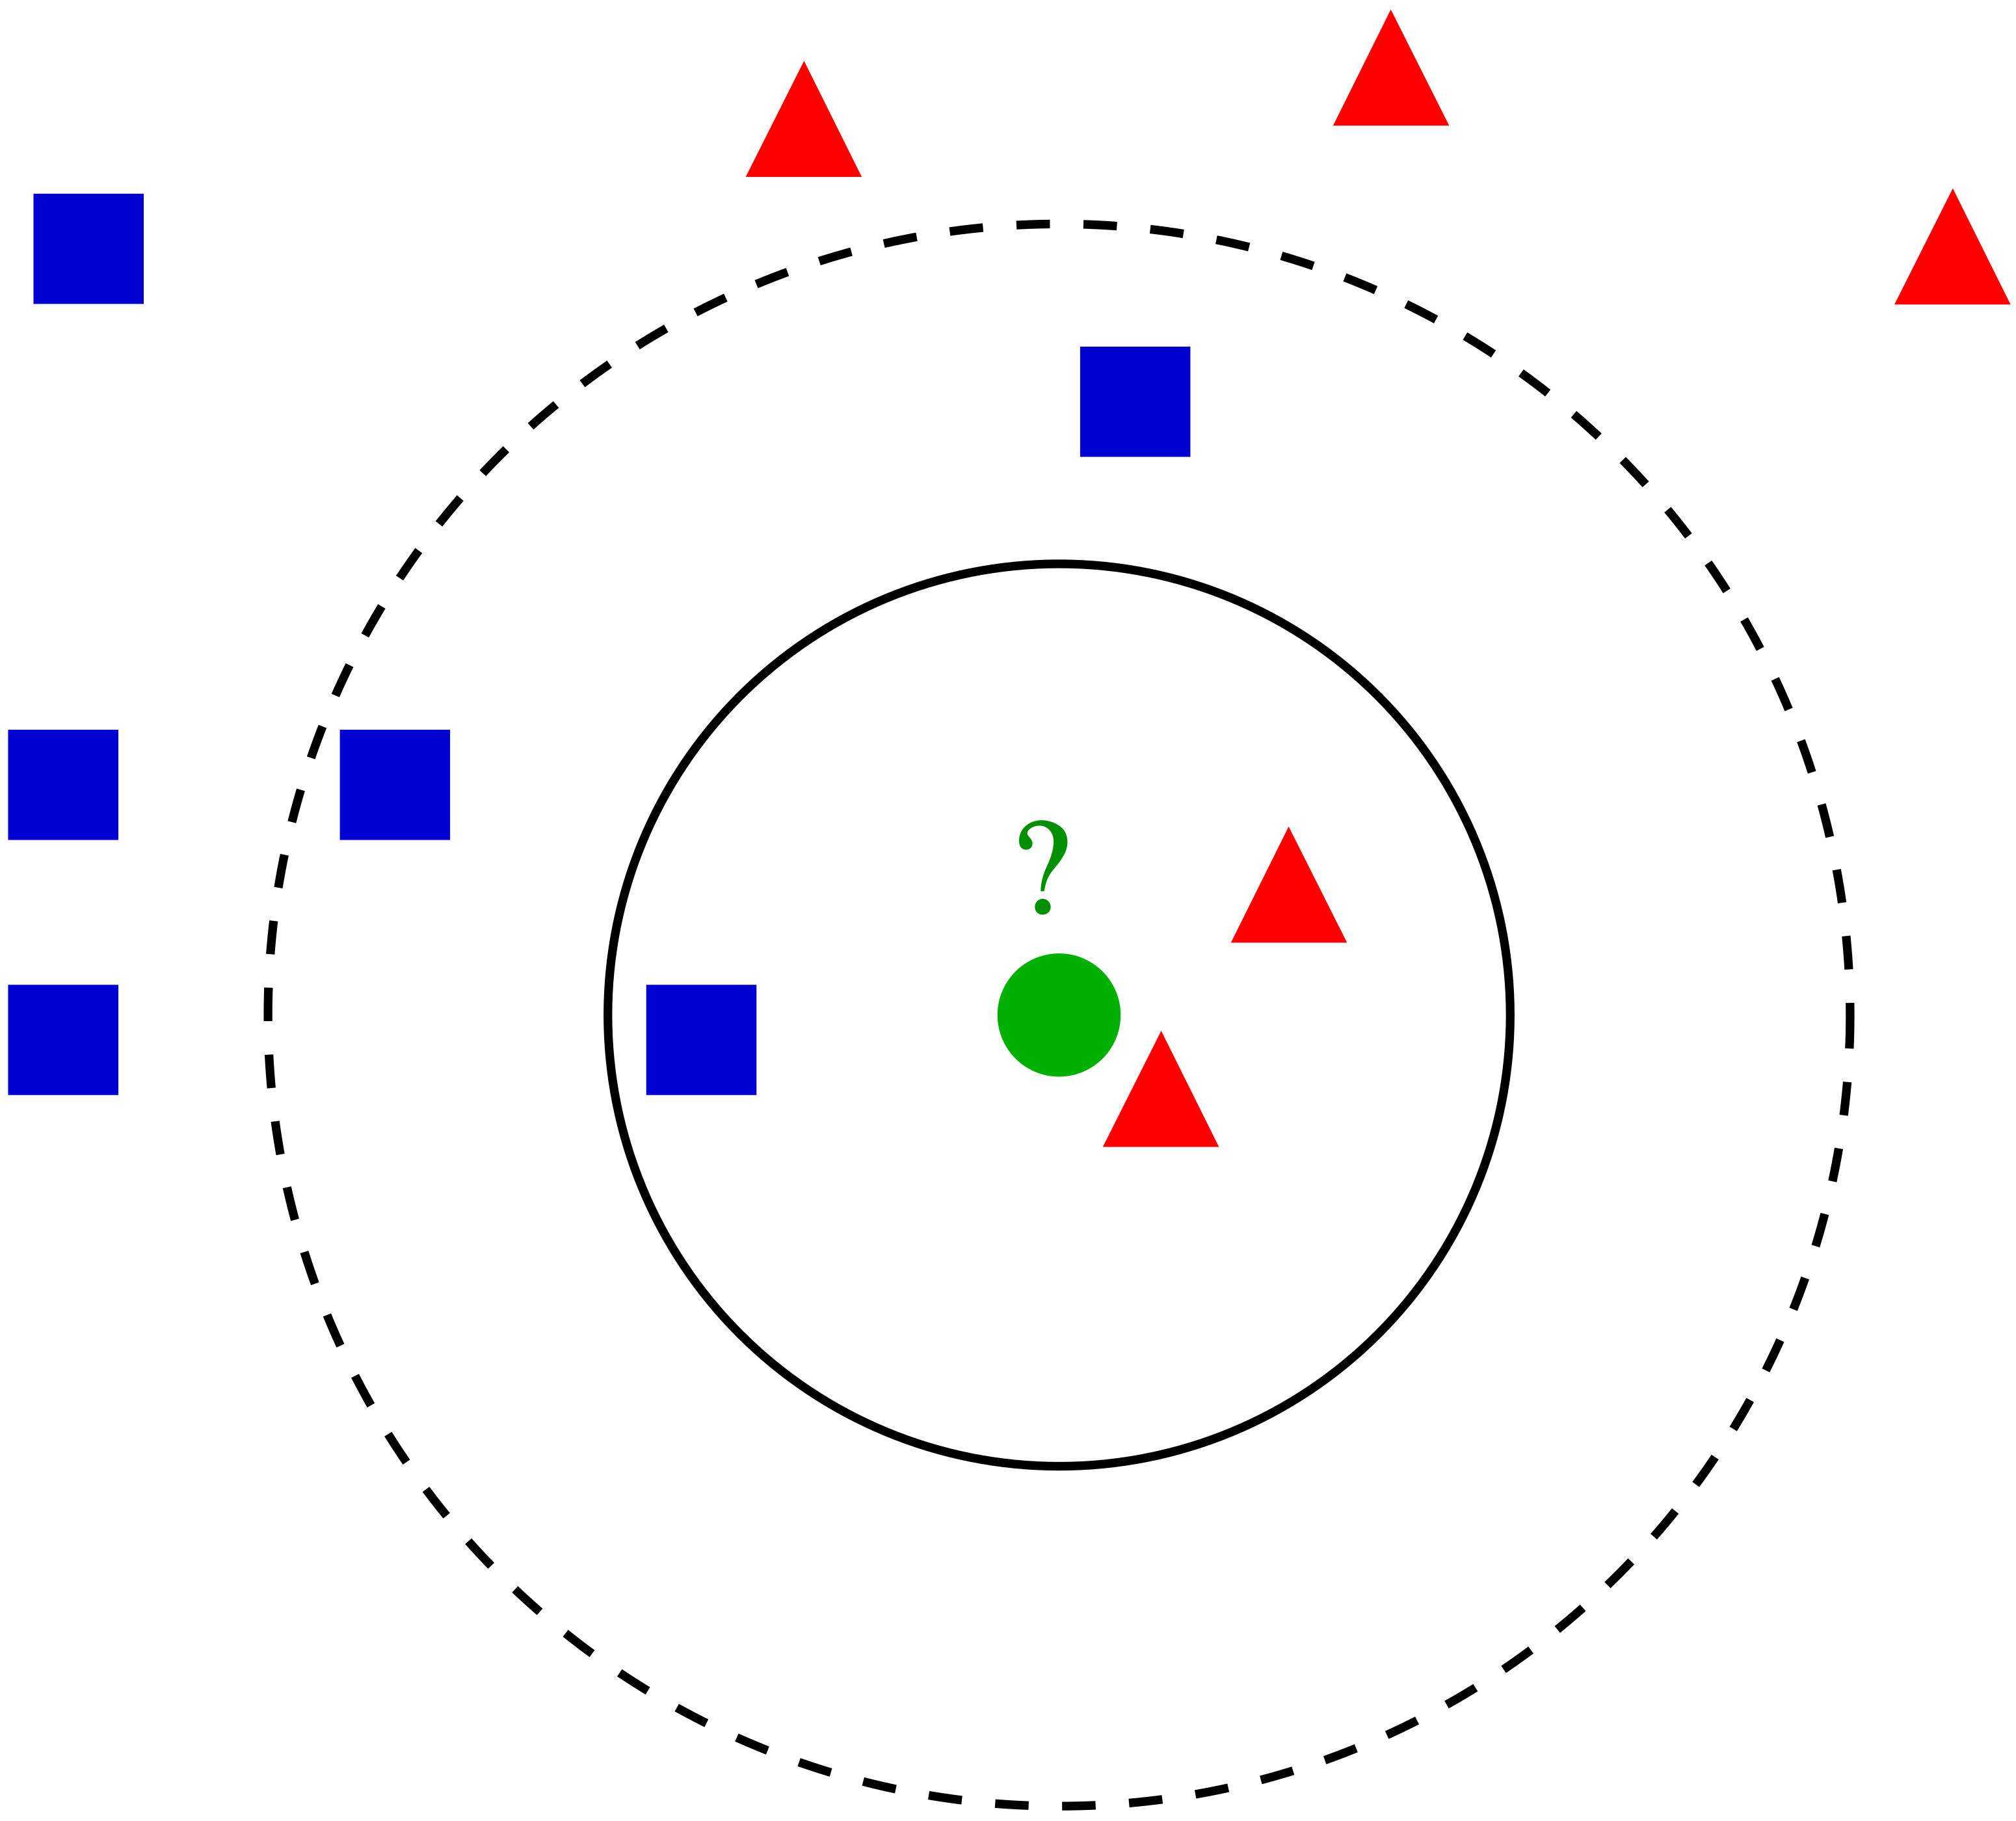
\includegraphics[width=.6\columnwidth]{gfx/KnnClassification.png}
            \end{center}

            \column{0.6\textwidth}

            Dato un insieme di vettori di training 
            \begin{equation*}
                \begin{split}
                    &D = v_0,\ldots,v_{M-1}, \\
                    &v_i\in\left\{ \text{classe}_0, \text{classe}_1, \ldots \right\}
                \end{split}
            \end{equation*}

            Dato un nuovo vettore $x$: 
            \begin{itemize}
                \item considera i $k$ vettori di training più vicini ad $x$
                \item classifica $x$ con un voto a maggioranza
            \end{itemize}

            Si assegnano pesi dipendenti da $\frac{1}{\text{distanza}}$ per aumentare l'influenza 
            dei vettori più vicini
        \end{columns}
    \end{frame}

    \begin{frame}{Algoritmo KNN quantistico}
        Stato quantistico iniziale: $\ket{a} \otimes \ket{i} \otimes \ket{c} \otimes \ket{m}$

		\begin{equation*}
			\ket{\psi_0} = \frac{1}{\sqrt{2M}} \sum_{m=1}^M 
			(\ket{0}\ket{\psi_x}+\ket{1}\ket{\psi_{t^m}})\ket{c^m}\ket{m}
		\end{equation*}

		Calcolo della distanza: \\ si fanno interferire gli stati applicando $H\ket{a}$
		\begin{equation*}
			\ket{\psi_1} = \frac{1}{2\sqrt{M}}\sum_{m=1}^M 
			\Big[ \ket{0}(\ket{\psi_x}+\ket{\psi_{t^m}}) + \ket{1}(\ket{\psi_x}-\ket{\psi_{t^m}}) \Big] \ket{c^m}\ket{m}
		\end{equation*}
	
		Misura condizionale: $\ket{a} = \ket{0}$

		\begin{equation*}
			\ket{\psi_2} = \frac{1}{2\sqrt{M}} \sum_{m=1}^M \sum_{i=1}^N
			(x_i+t_i^m)\ket{0}\ket{i}\ket{c^m}\ket{m}
		\end{equation*}
    \end{frame}

    \begin{frame}{Algoritmo KNN quantistico}
        Se i vettori sono appropriatamente normalizzati 
        la probabilità di misurare una data classe è:

		\begin{equation*}
			\text{P}(\ket{c^m} = \ket{s}) = 1 - \sum_{m|c^m=s} 
			\frac{1}{4M} |x-t^m|^2
		\end{equation*}

		Classificazione:

		\begin{equation*}
			c = \begin{cases}
			0 \quad \text{se}\, \text{P}(\ket{c^0})\, \text{maggiore} \\
			1 \quad \text{se}\, \text{P}(\ket{c^1})\, \text{maggiore} \\
			\text{etc}\ldots
		\end{cases}
        \end{equation*}
    \end{frame}

    \begin{frame}{Algoritmo KNN quantistico}
        \begin{center}
            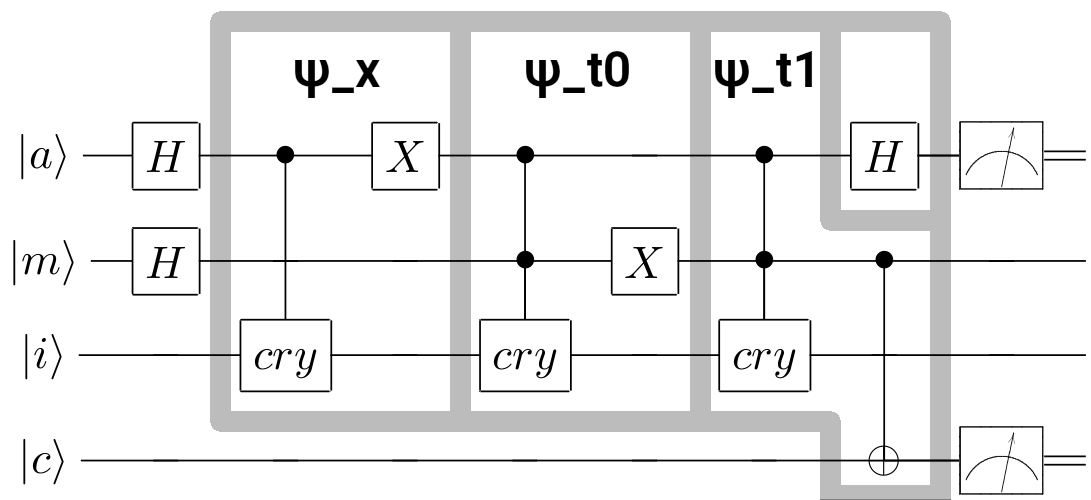
\includegraphics[width=.8\textwidth]{gfx/qknn_boxes.png}            
        \end{center}

        La complessità algoritmica del procedimento, ignorando la preparazione dello 
        stato, è $\mathcal{O}\left(\frac{1}{\text{P(MC)}}\right)$, 
        dove $\text{P(MC)}$ è la probabilità di successo della misura condizionale 
        (misura dell'ancilla nello stato $\ket{0}$). 
        Dipendendo questa solo dalla configurazione iniziale del sistema, si 
        dice che l'algoritmo ha un tempo di esecuzione costante. \cite{fingerhuth}
    \end{frame}

    \begin{frame}{FF-QRAM}
        Per codificare dati classici nelle ampiezze di probabilità è stata usata la tecnica di costruzione 
        di stati flip-flop QRAM proposta da Petruccione et al. \cite{petruccione}
        La FF-QRAM è usata per inizializzare efficientemente un QDB in maniera arbitraria. 

        L'operazione QRAM sui qubit sovrappone un insieme di dati classici 
        $D = \left\{ \left( \vec{d}^{(l)}, b_l \right) \Big| 0 \leq l < M \right\}$ come
        \begin{equation*} \label{eq:qram}
            \text{QRAM}(D) \sum_j \psi_j \ket{j}_B \ket{0}_R \equiv 
            \sum_l \psi_l \ket{\vec{d}^{(l)}}_B \ket{b_l}_R,
        \end{equation*}
        dove $\vec{d}^{(l)}$ rappresenta un indirizzo di memoria con 
        $n$ bit di informazione 
        e $b_l$ è l'attributo ad esso associato (per es. numero reale). 
    \end{frame}

    \begin{frame}{Codificare dati classici nelle ampiezze}
        \begin{columns}
            \column{.4\textwidth}
            La complessità algoritmica di questa routine è $\mathcal{O}(MN)$, dove $M$ è il numero di 
            vettori e $N$ la loro lunghezza. La quantità di risorse hardware necessarie va 
            come $\mathcal{O}(\log_2(MN))$. \cite{petruccione} 
            \column{.6\textwidth}
            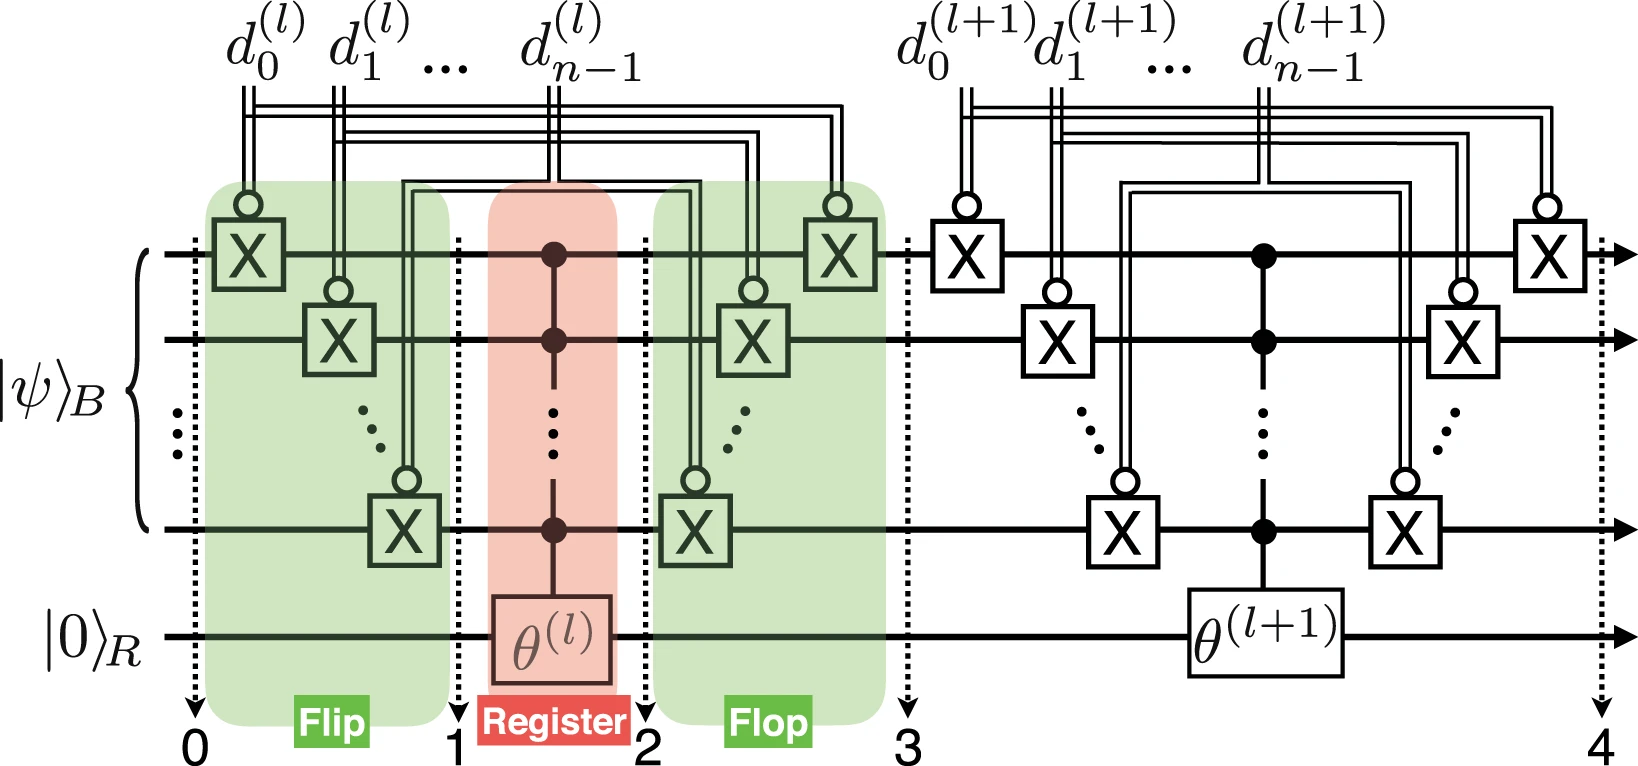
\includegraphics[width=\columnwidth]{gfx/qram}
        \end{columns}

        \begin{columns}
            \column{.4\textwidth}
            Per codificare più di due classi una procedura di tipo QRAM risulta conveniente. 
            \column{.6\textwidth}
            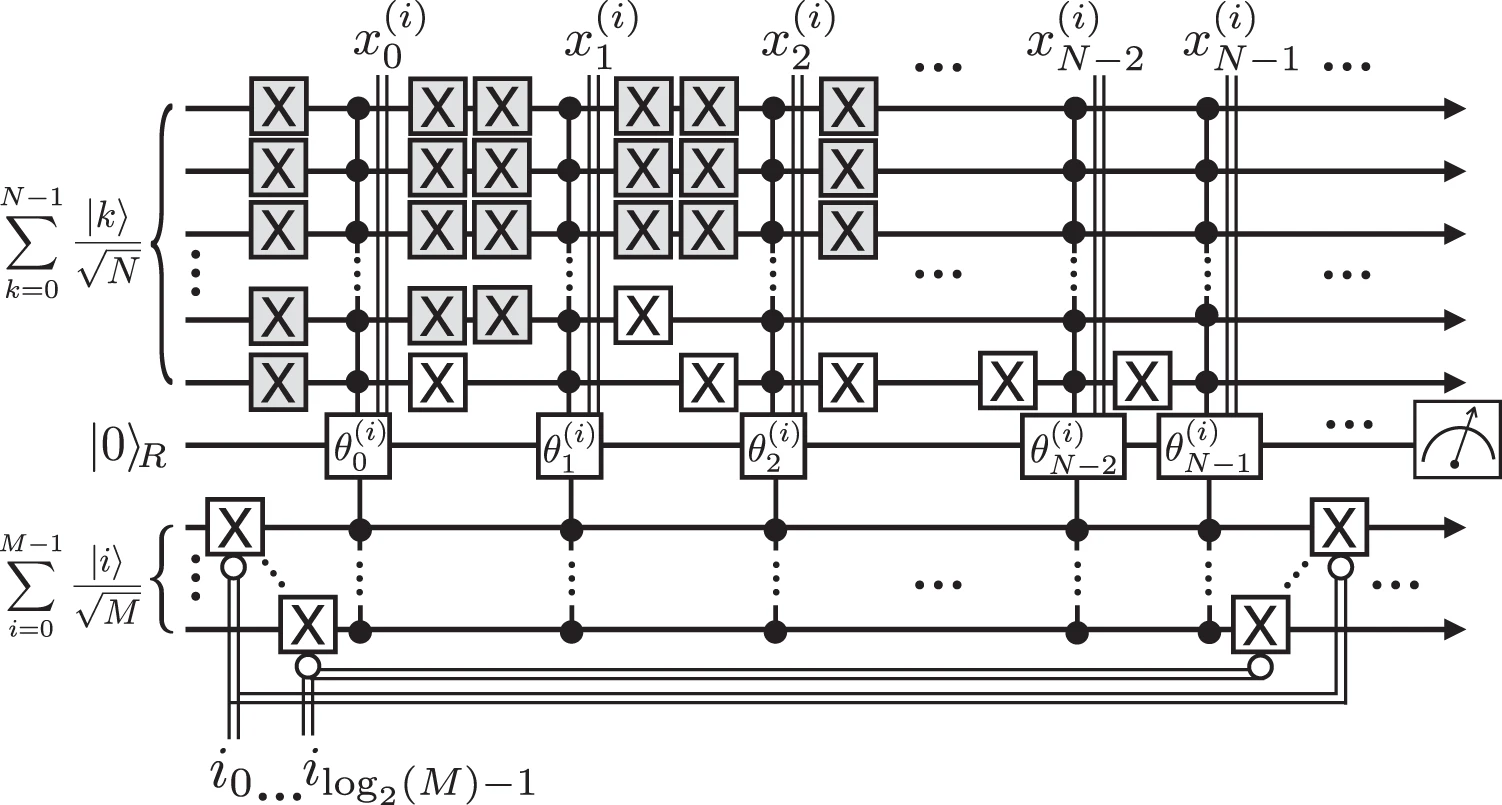
\includegraphics[width=\columnwidth]{gfx/qram_qsvm}
        \end{columns}
    \end{frame}

    \begin{frame}[t]{Metodi}
        \begin{minipage}[t]{.45\textwidth}
            \vspace{0pt}
            \begin{center}
                Qiskit
            \end{center}
            Struttura open source di sviluppo software \cite{Qiskit} per 
            \begin{itemize}
                \item progettare circuiti quantistici
                \item simularli sul proprio computer personale
                \item inviare ordini di esecuzione su harware quantistico reale
                \item visualizzare i risultati
            \end{itemize}
        \end{minipage}
        \hfill
        \begin{minipage}[t]{.45\textwidth}
            \vspace{0pt}
            \begin{center}
                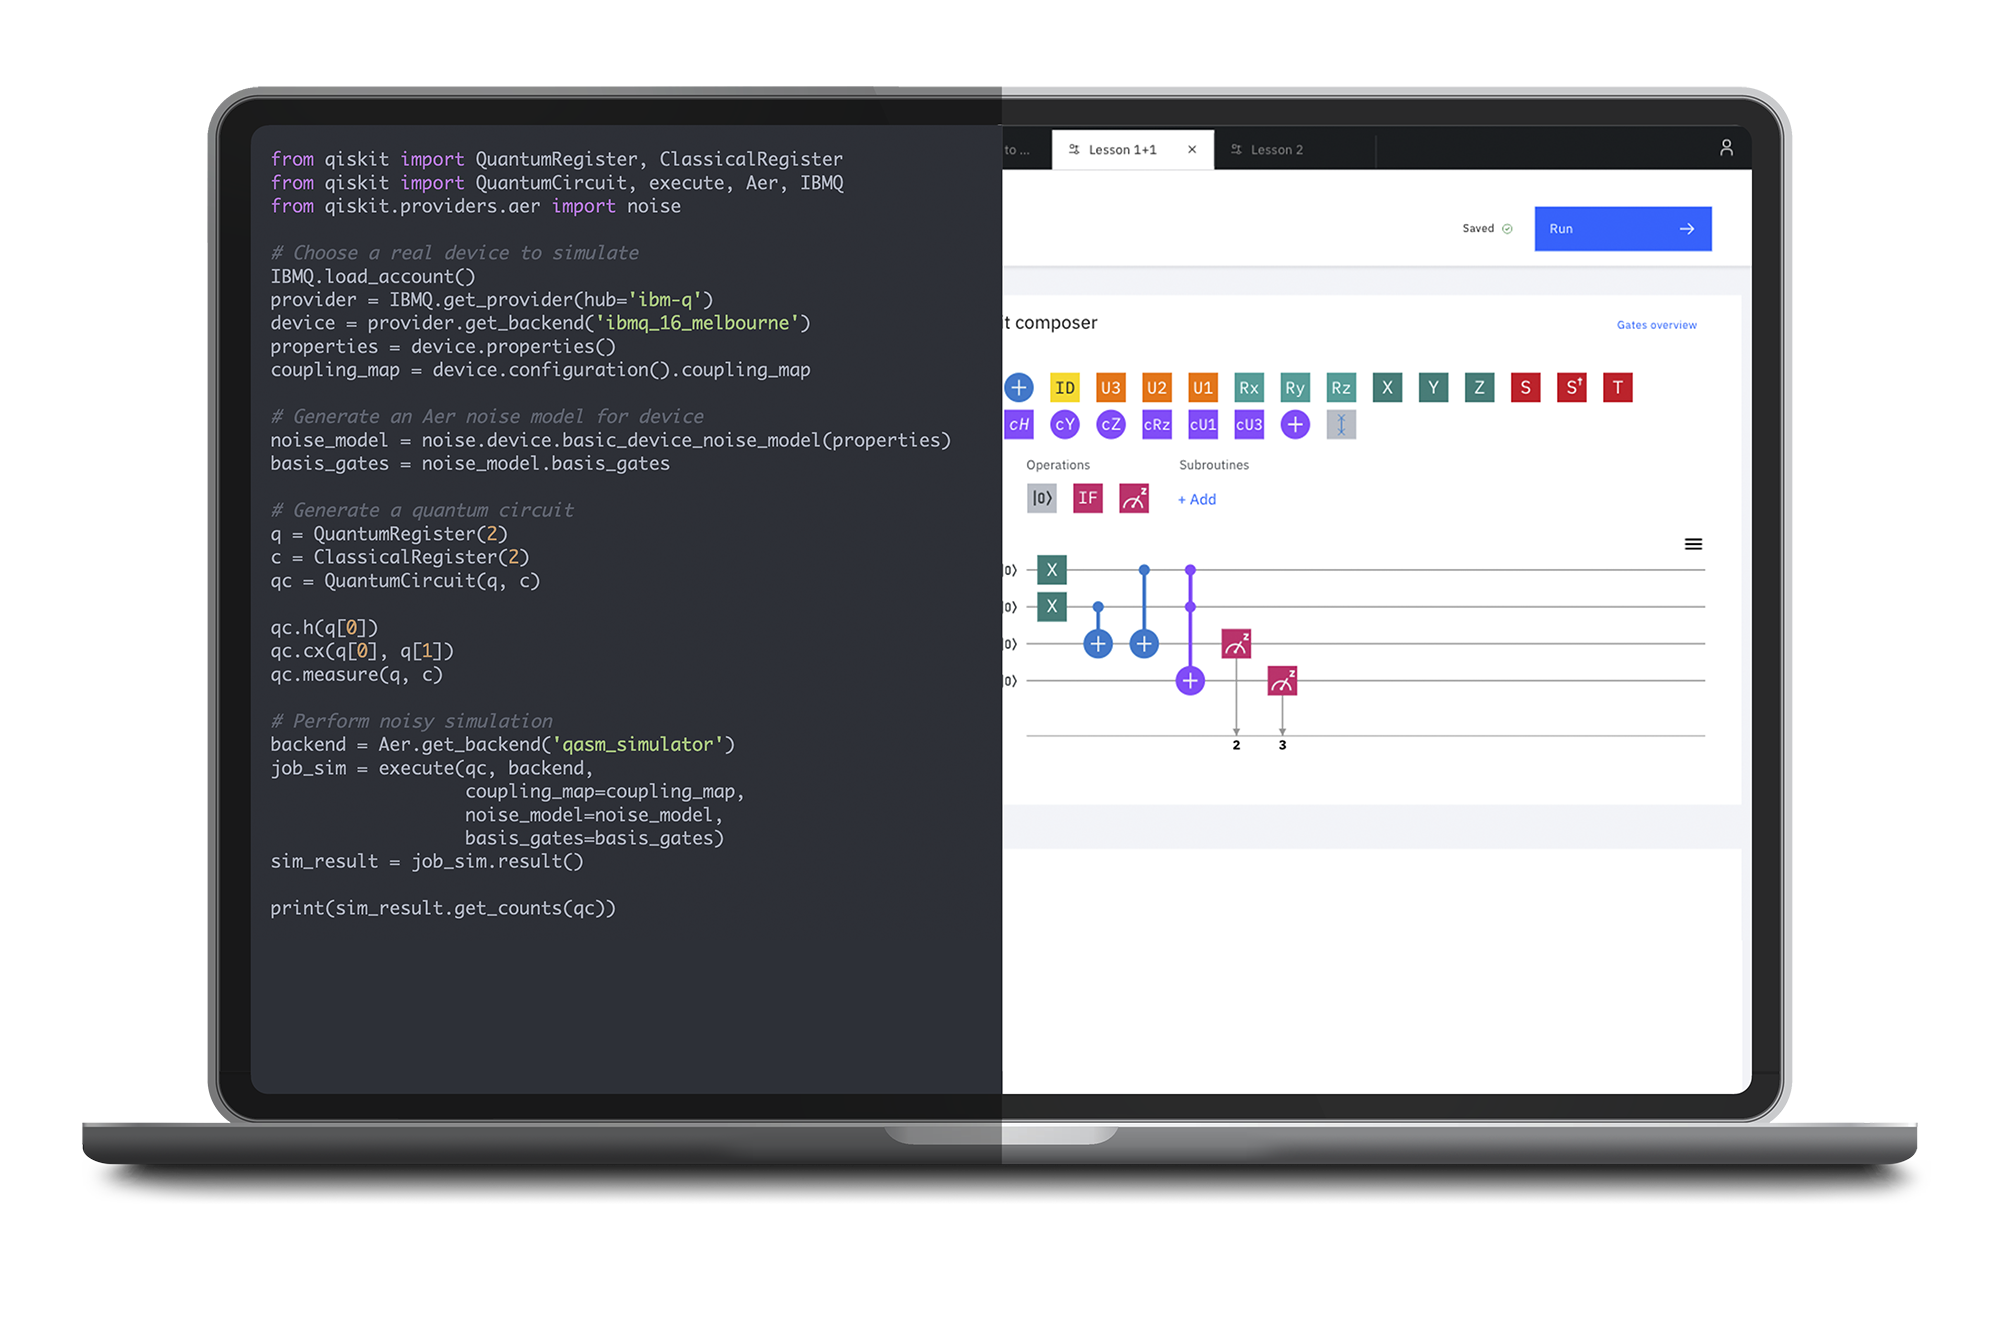
\includegraphics[width=.6\columnwidth]{gfx/laptop_strumenti.png}
            \end{center}
            \begin{center}
                IBM Q Experience
            \end{center}
            \begin{itemize}
                \item accessibile al pubblico
                \item permette simulazioni ideali e con rumore
                \item fino a 14 qubit superconduttivi
                \item fino a 32 qubit simulati
            \end{itemize}
        \end{minipage}
    \end{frame}

    \begin{comment}
    \begin{frame}{IBM Q Experience}
        \begin{columns}
            \column{.3\textwidth}
            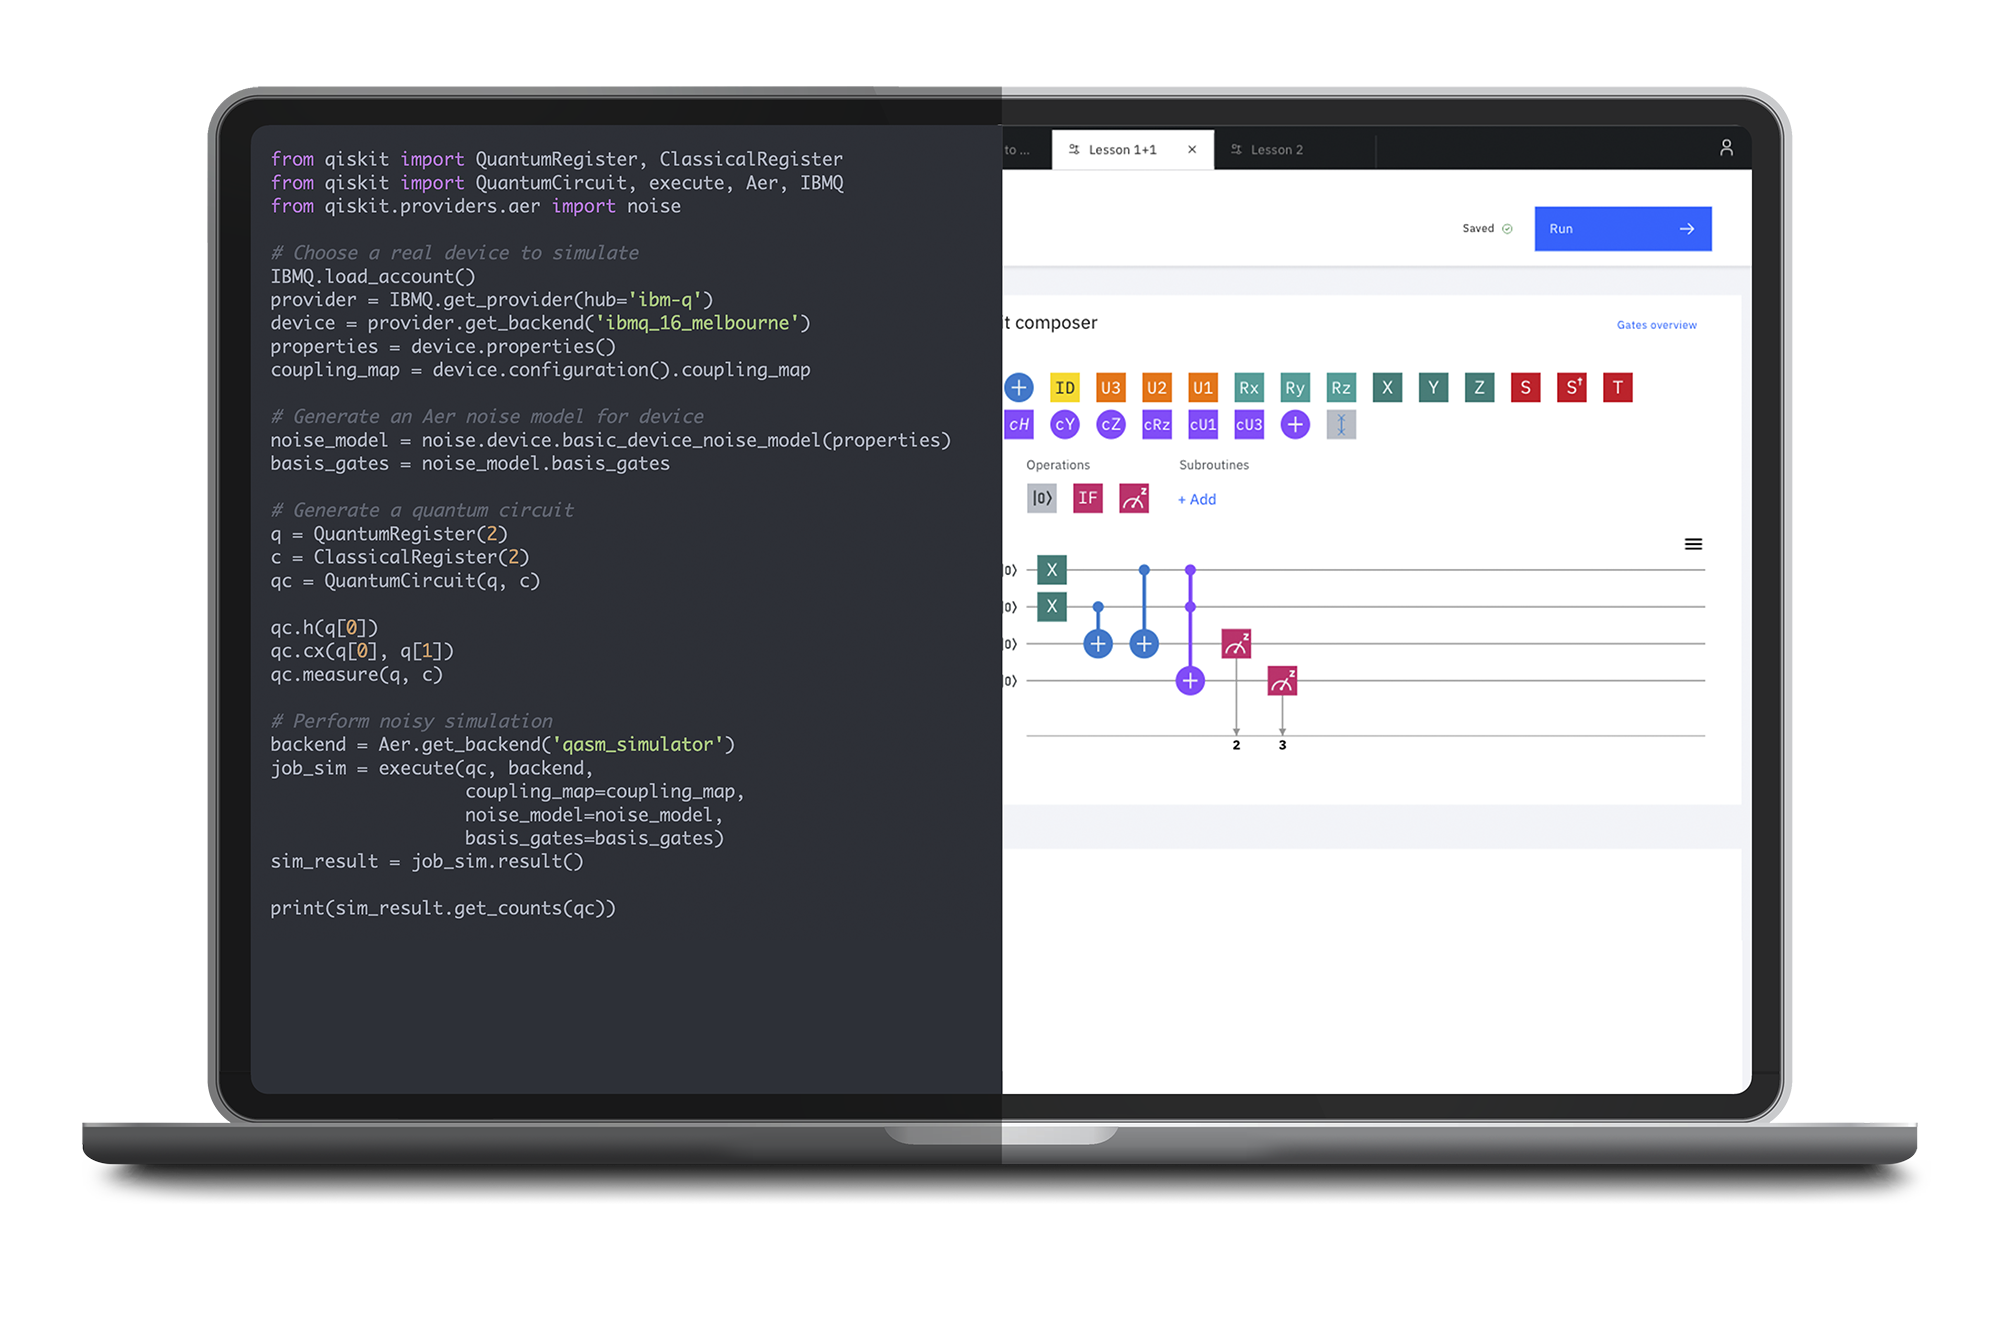
\includegraphics[width=\textwidth]{gfx/laptop_strumenti.png}
            \column{.7\textwidth}
            L'IBM Q Experience è un'interfaccia per interagire con le risorse di quantum computing dell'IBM
            \begin{itemize}
                \item accessibile al pubblico
                \item permette simulazioni con e senza rumore
                \item fino a 14 qubit superconduttivi
                \item fino a 32 qubit simulati
            \end{itemize}
        \end{columns}
    \end{frame}

    \begin{frame}{Qiskit}
        \begin{columns}
            \column{.3\textwidth}
            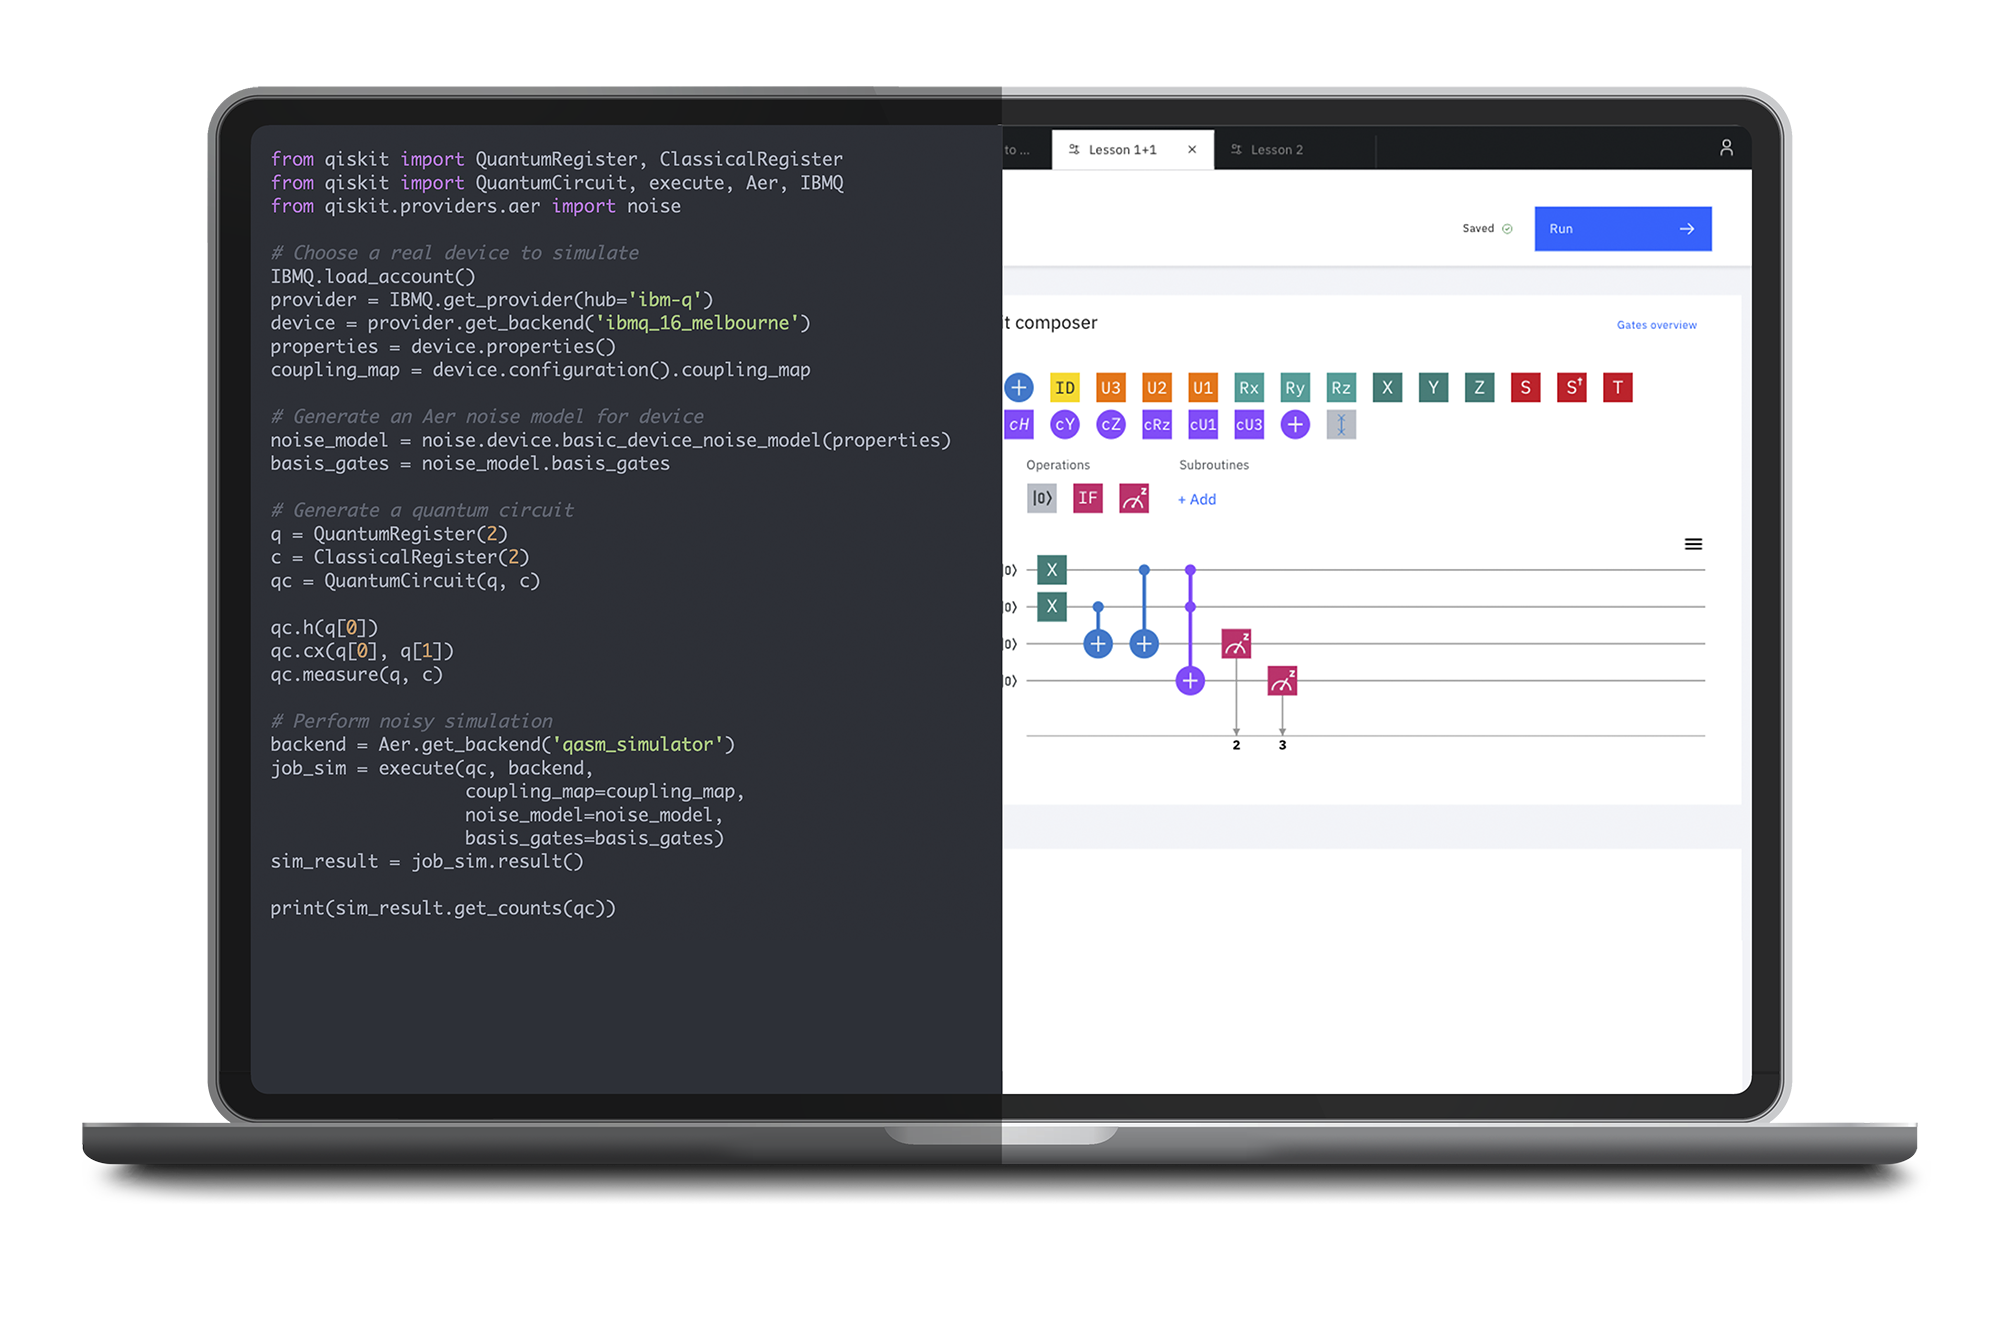
\includegraphics[width=\textwidth]{gfx/laptop_strumenti.png}
            \column{.7\textwidth}
            Struttura open source di sviluppo software per quantum computing \cite{Qiskit}, permette di 
            \begin{itemize}
                \item progettare circuiti quantistici
                \item simularli sul proprio computer personale
                \item inviare ordini di esecuzione su harware quantistico reale
                \item visualizzare i risultati
            \end{itemize}
        \end{columns}
    \end{frame}
    \end{comment}

    \begin{frame}{Stato dell'arte}
        \begin{columns}
            \column{.3\textwidth}
            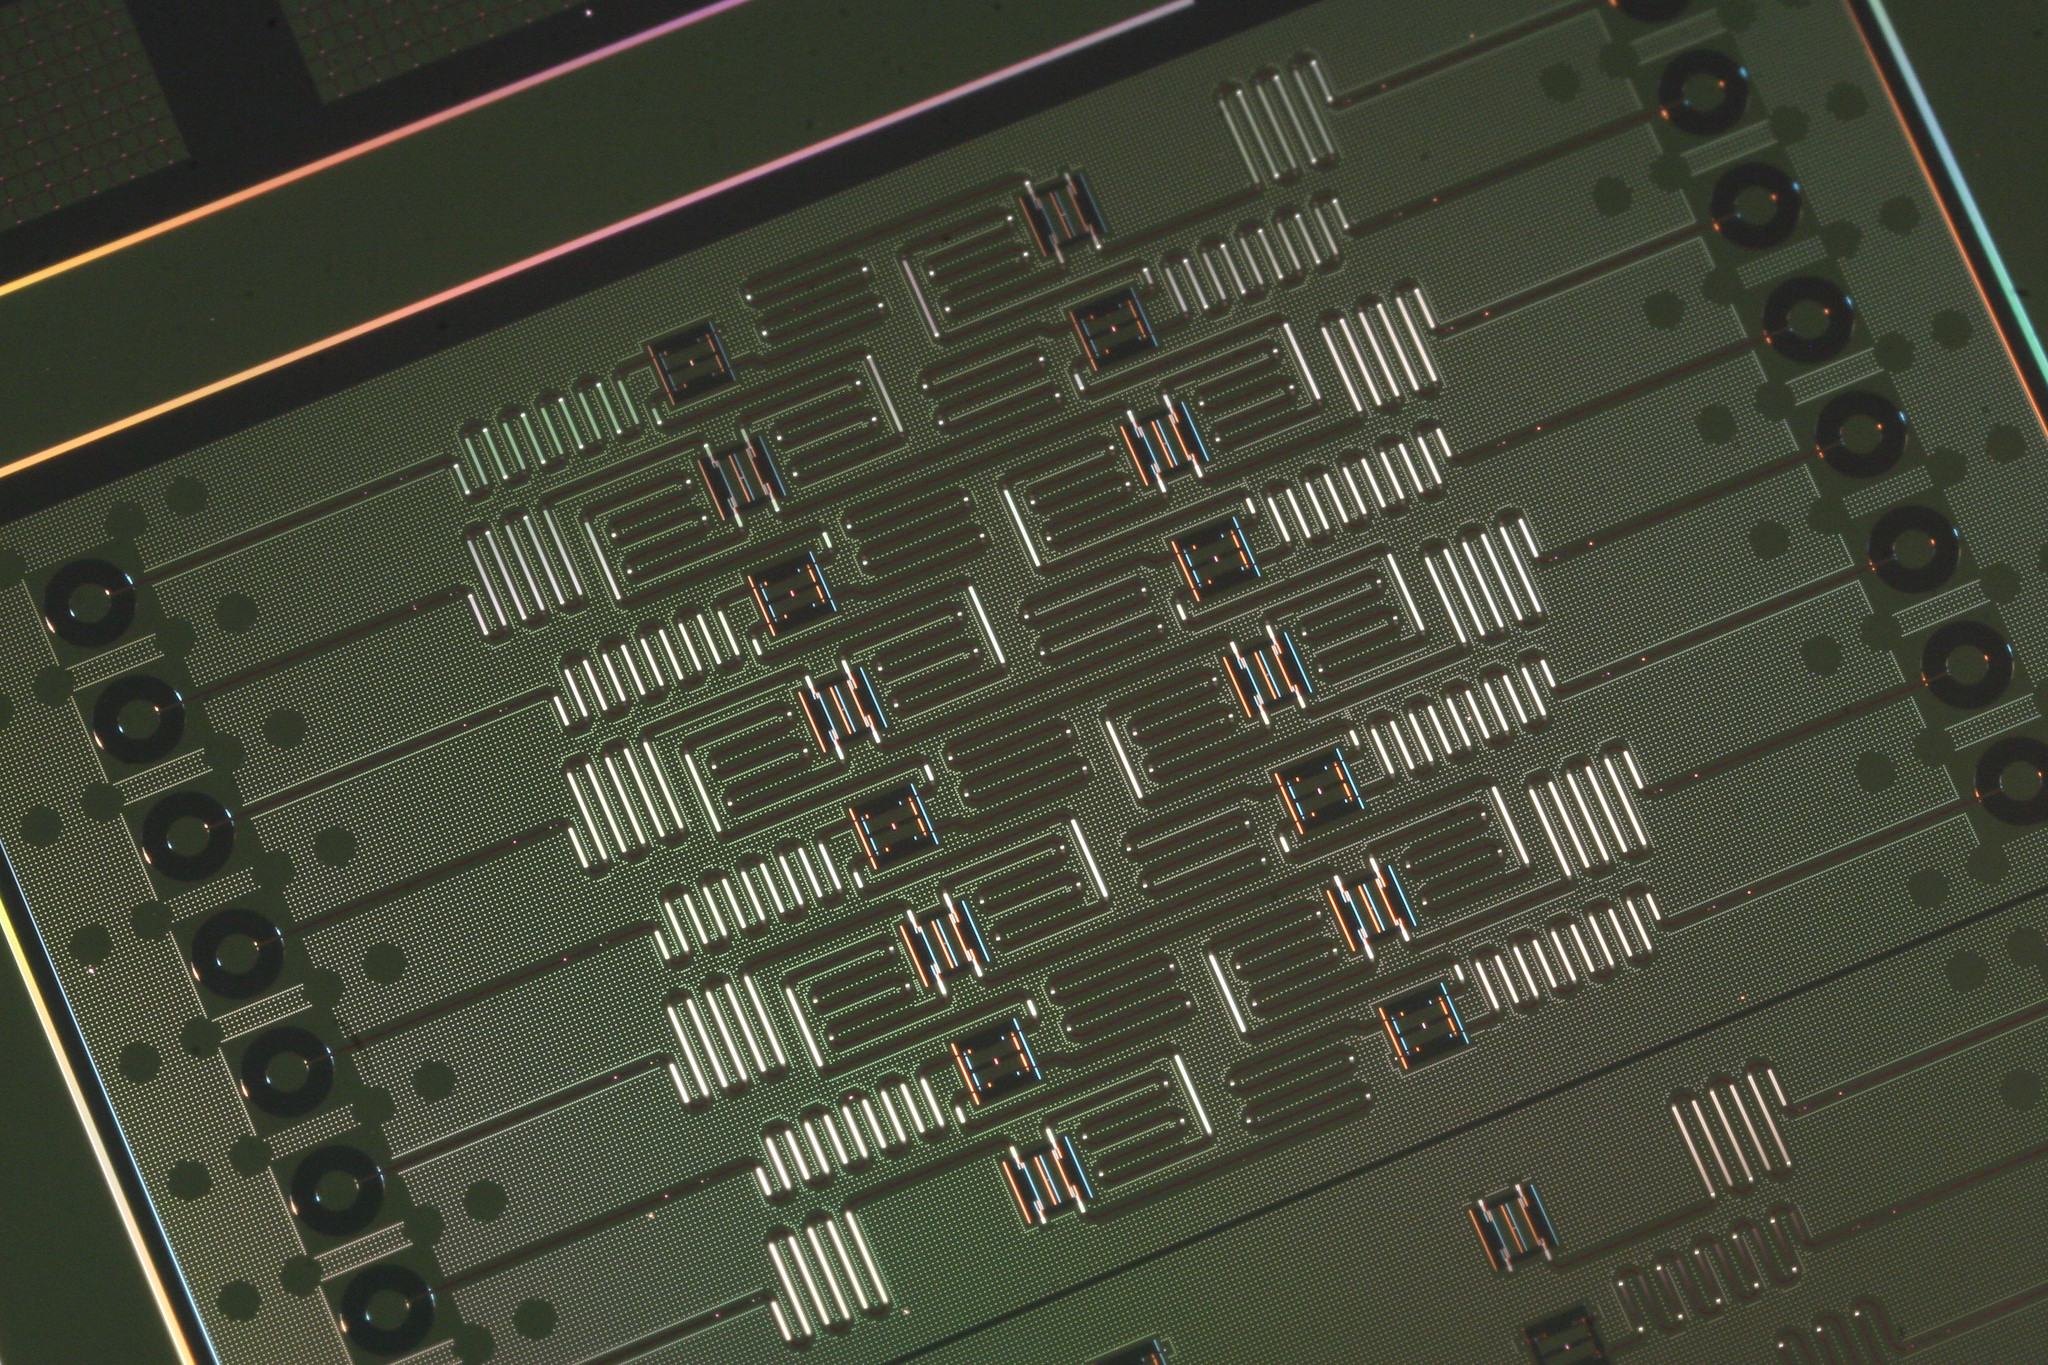
\includegraphics[width=\textwidth]{gfx/ibm_16}
            \column{.7\textwidth}
            L'ibmq\_16\_melbourne è il computer quantistico accessibile al pubblico 
            a partire dal 2018 tramite interfaccia web. Le porte quantistiche di base 
            sono u1, u2, u3, cx, id. I tempi di decoerenza sono dell'ordine di 
            $T1 \approx 25 \div 88 \mu s$, $T2 \approx 15 \div 105 \mu s$. 
        \end{columns}

        \begin{columns}
            \column{.3\textwidth}
            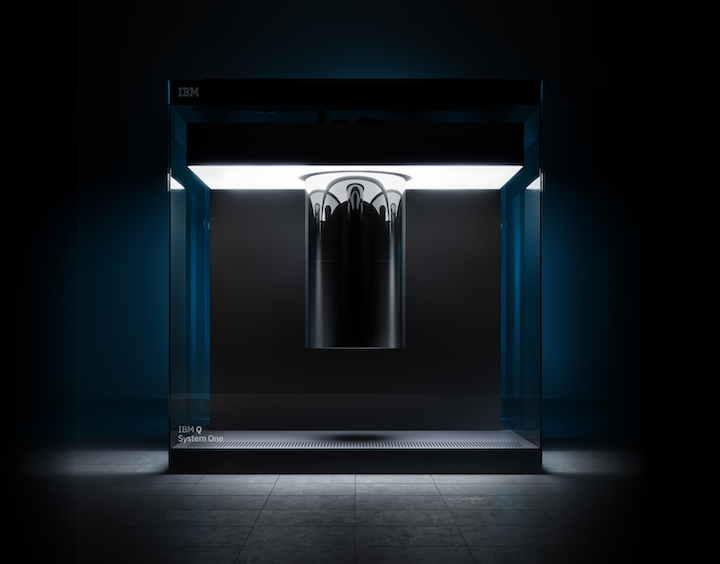
\includegraphics[width=\textwidth]{gfx/ibm_q_system_one.png}
            \column{.7\textwidth}
            L'IBM Q System One è il primo computer quantistico a circuiti commerciale al mondo, 
            introdotto dall'IBM nel gennaio 2019. L'IBM Q System One possiede 20 qubit. 
        \end{columns}
    \end{frame}

    \section*{Risultati}
    \subsection{Classificazione di cluster}

    \begin{frame}{Classificazione di cluster}
        \begin{columns}
            \column{.5\textwidth}
            Per verificare il funzionamento base dell'algoritmo, è stato creato un insieme dati ad hoc formato da quattro raggruppamenti ben separati tra loro. 
            \column{.5\textwidth}
            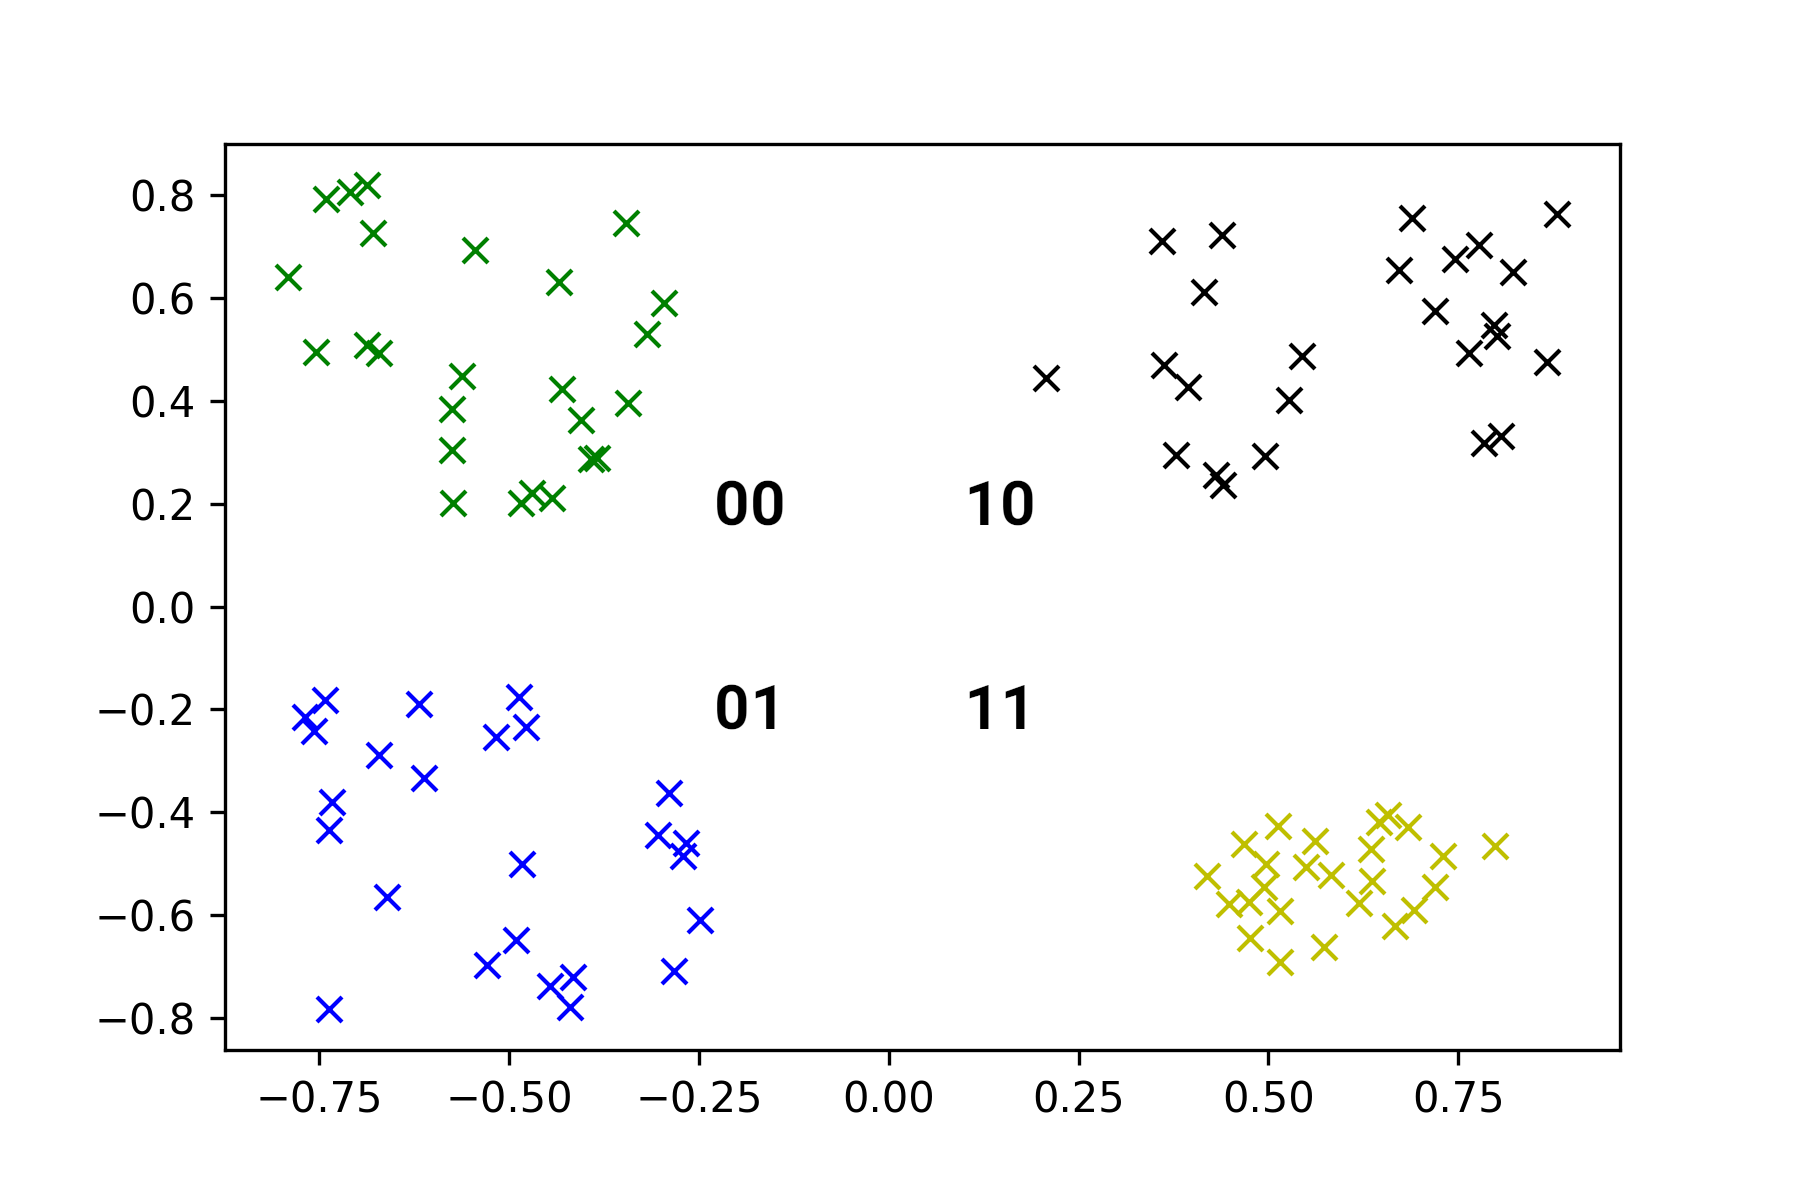
\includegraphics[width=\columnwidth]{gfx/Clusters/cluster_numbered.png}
    \end{columns}

    \begin{columns}
        \column{.5\textwidth}
        Sono stati selezionati otto elementi (due da ogni cluster) come vettori di training 
        e si sono sottoposti a classificazione un vettore d'input di ciascuna classe in quattro esperimenti. 
        \column{.5\textwidth}
        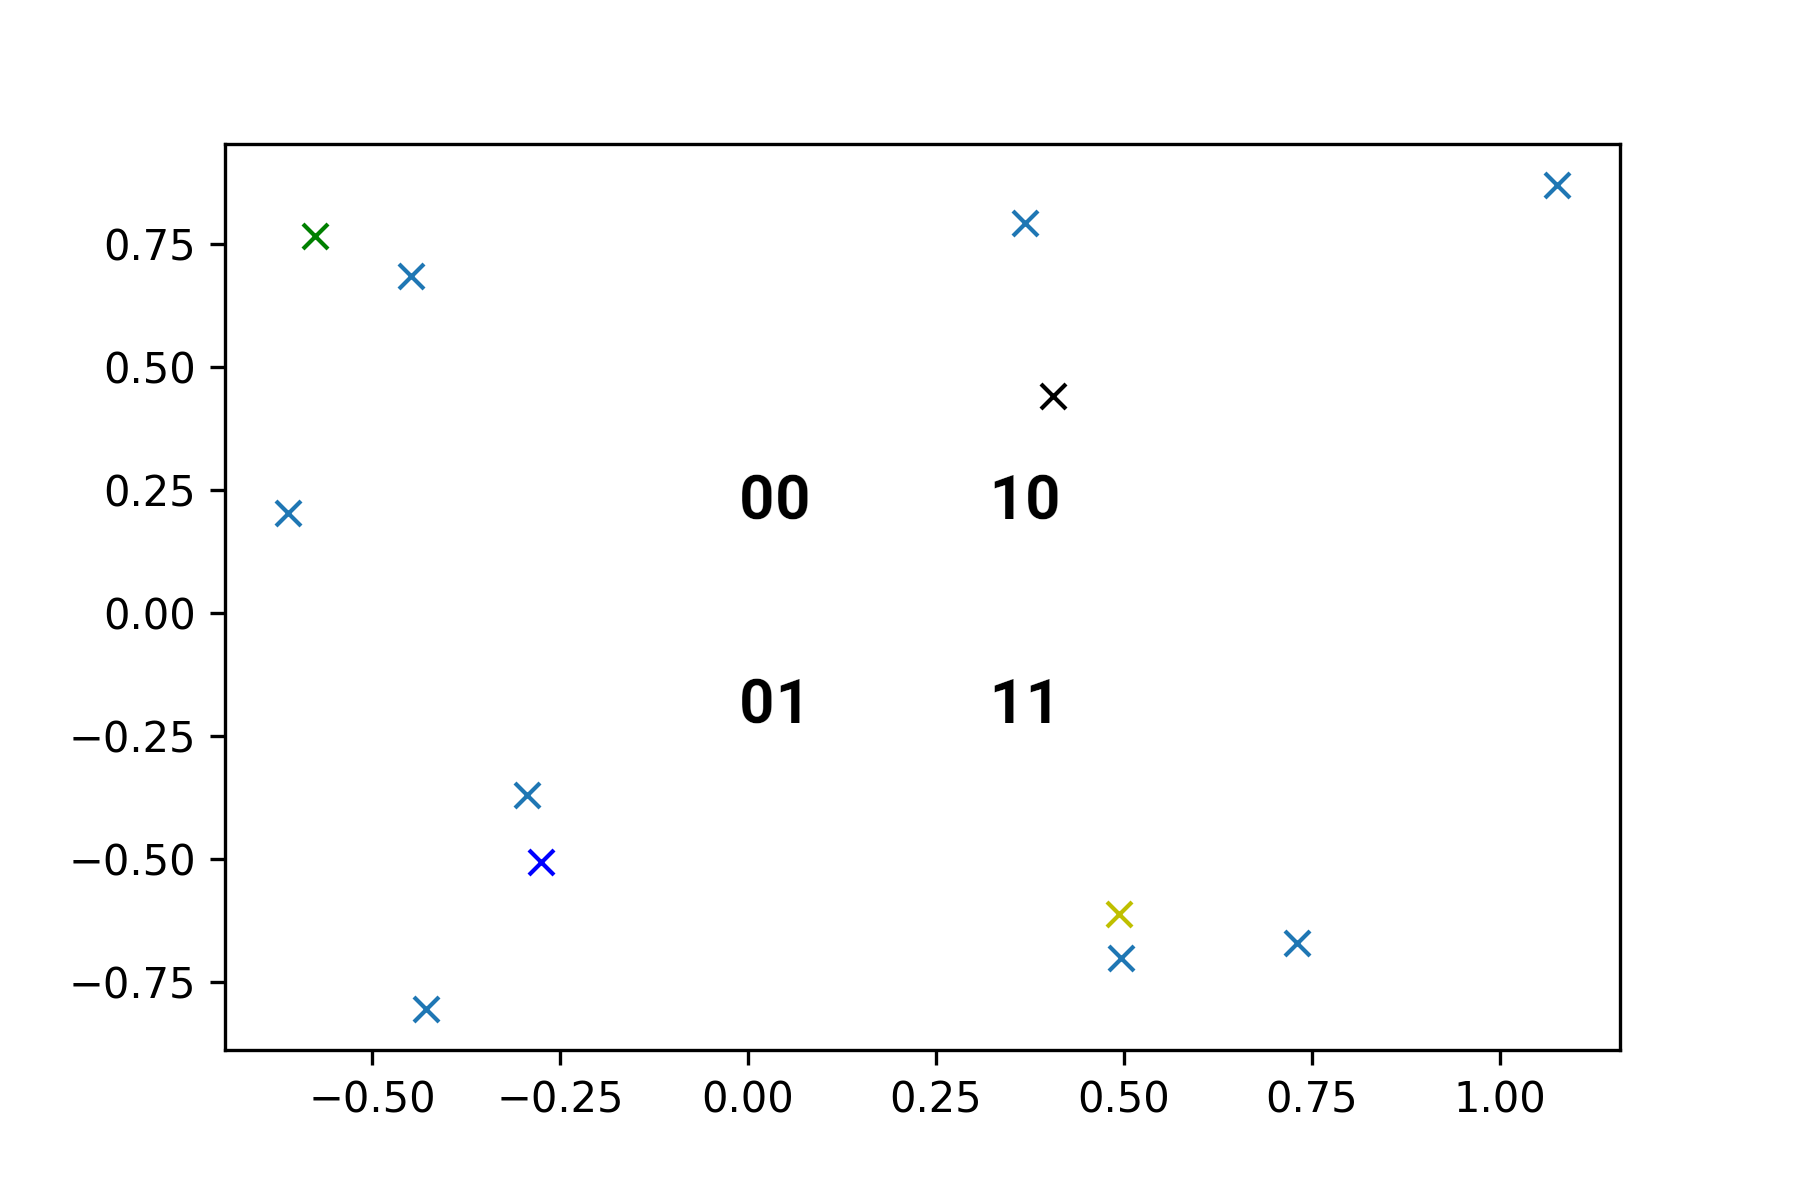
\includegraphics[width=\columnwidth]{gfx/Clusters/random_numbered.png}            
    \end{columns}
    \end{frame}

    \begin{frame}{Classificazione di cluster (simulazione)}
        \begin{columns}
            \column{.5\linewidth}
            \rotatebox{90}{Classe verde}
            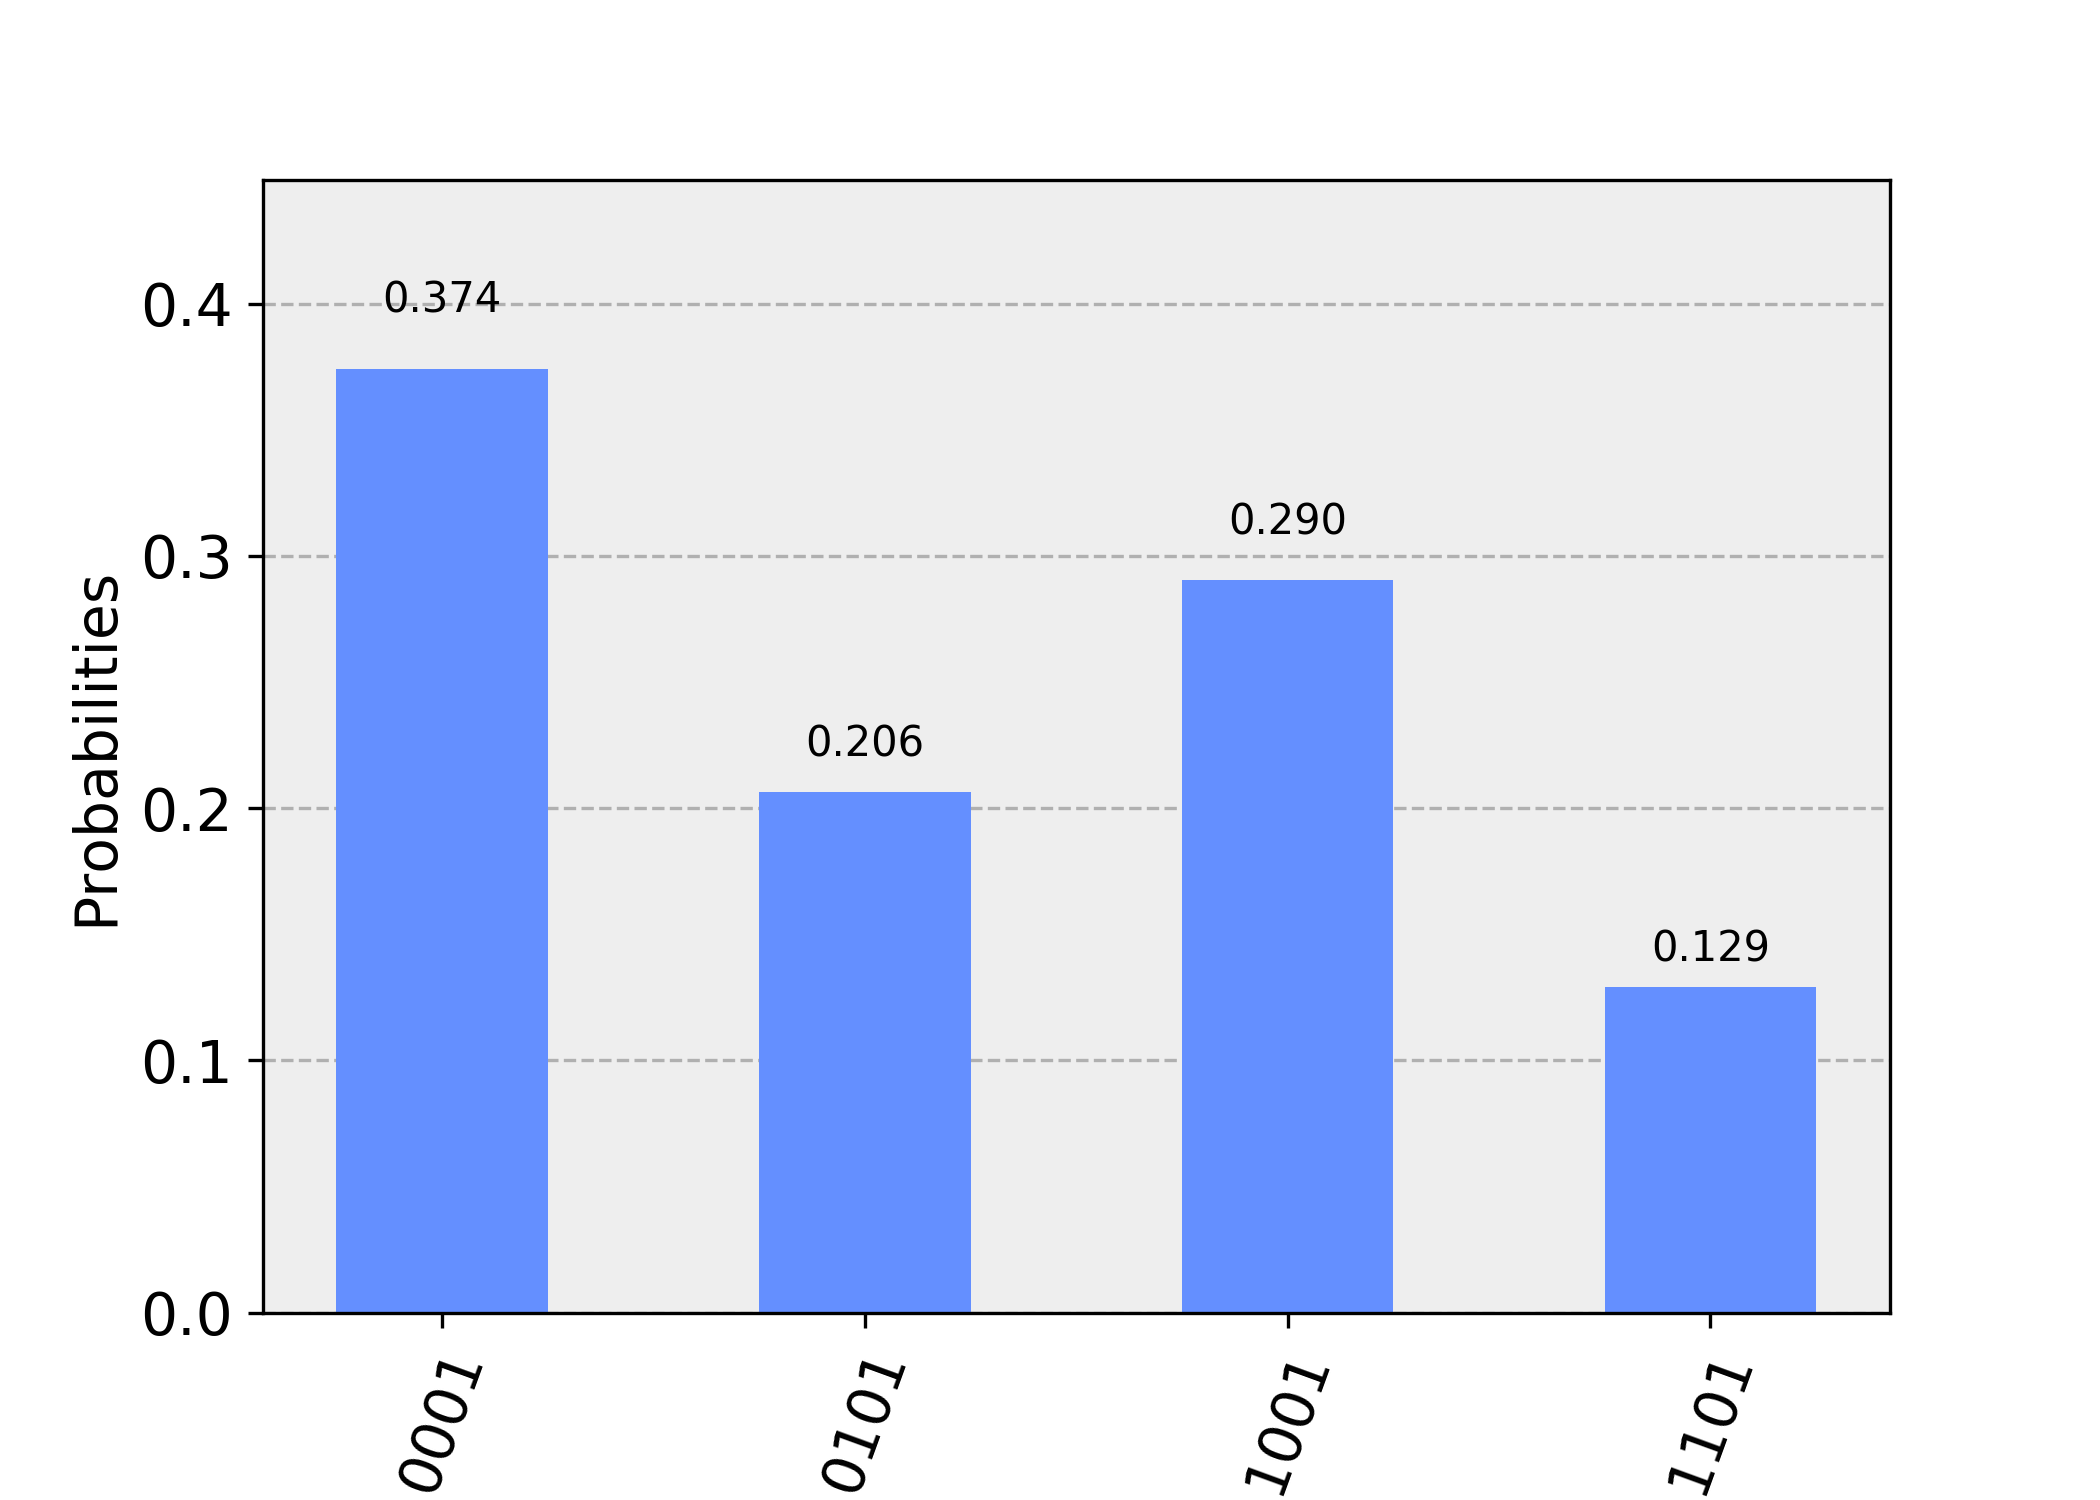
\includegraphics[width=.9\linewidth]{gfx/Clusters/Simulated/green}
            \rotatebox{90}{Classe blu}
            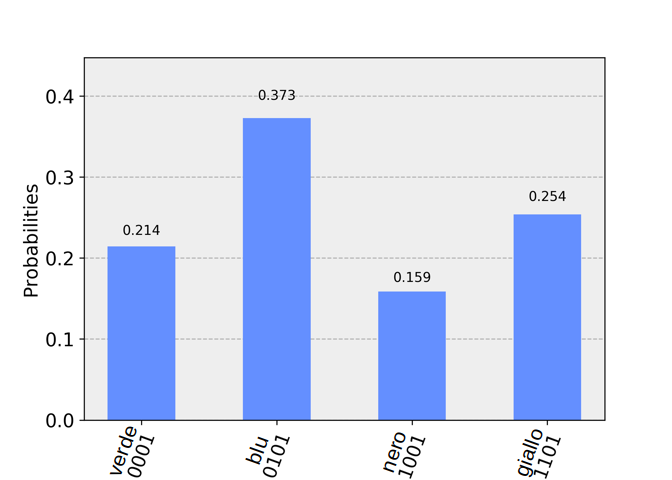
\includegraphics[width=.9\linewidth]{gfx/Clusters/Simulated/blue}
            \column{.5\linewidth}
            \rotatebox{90}{Classe nero}
            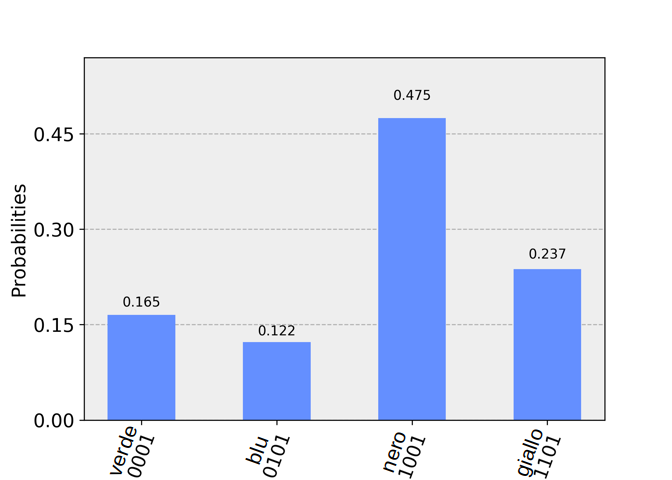
\includegraphics[width=.9\linewidth]{gfx/Clusters/Simulated/black}
            \rotatebox{90}{Classe giallo}
            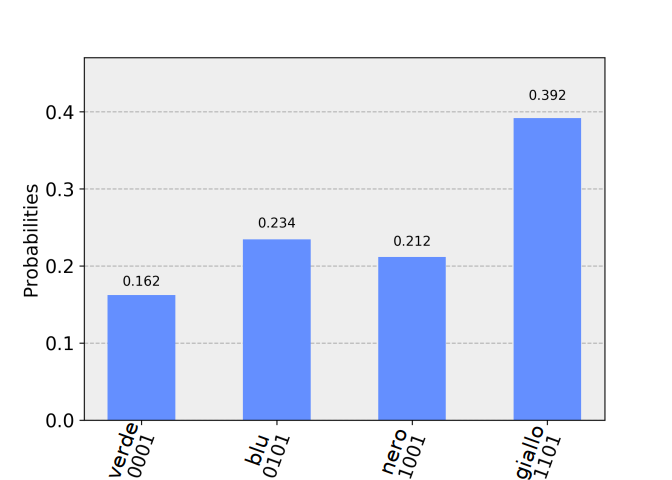
\includegraphics[width=.9\linewidth]{gfx/Clusters/Simulated/yellow}
        \end{columns}
    \end{frame}

    \subsection{Data set Iris}

    \begin{frame}{Data set Iris}
        \begin{columns}
            \column{.4\textwidth}
            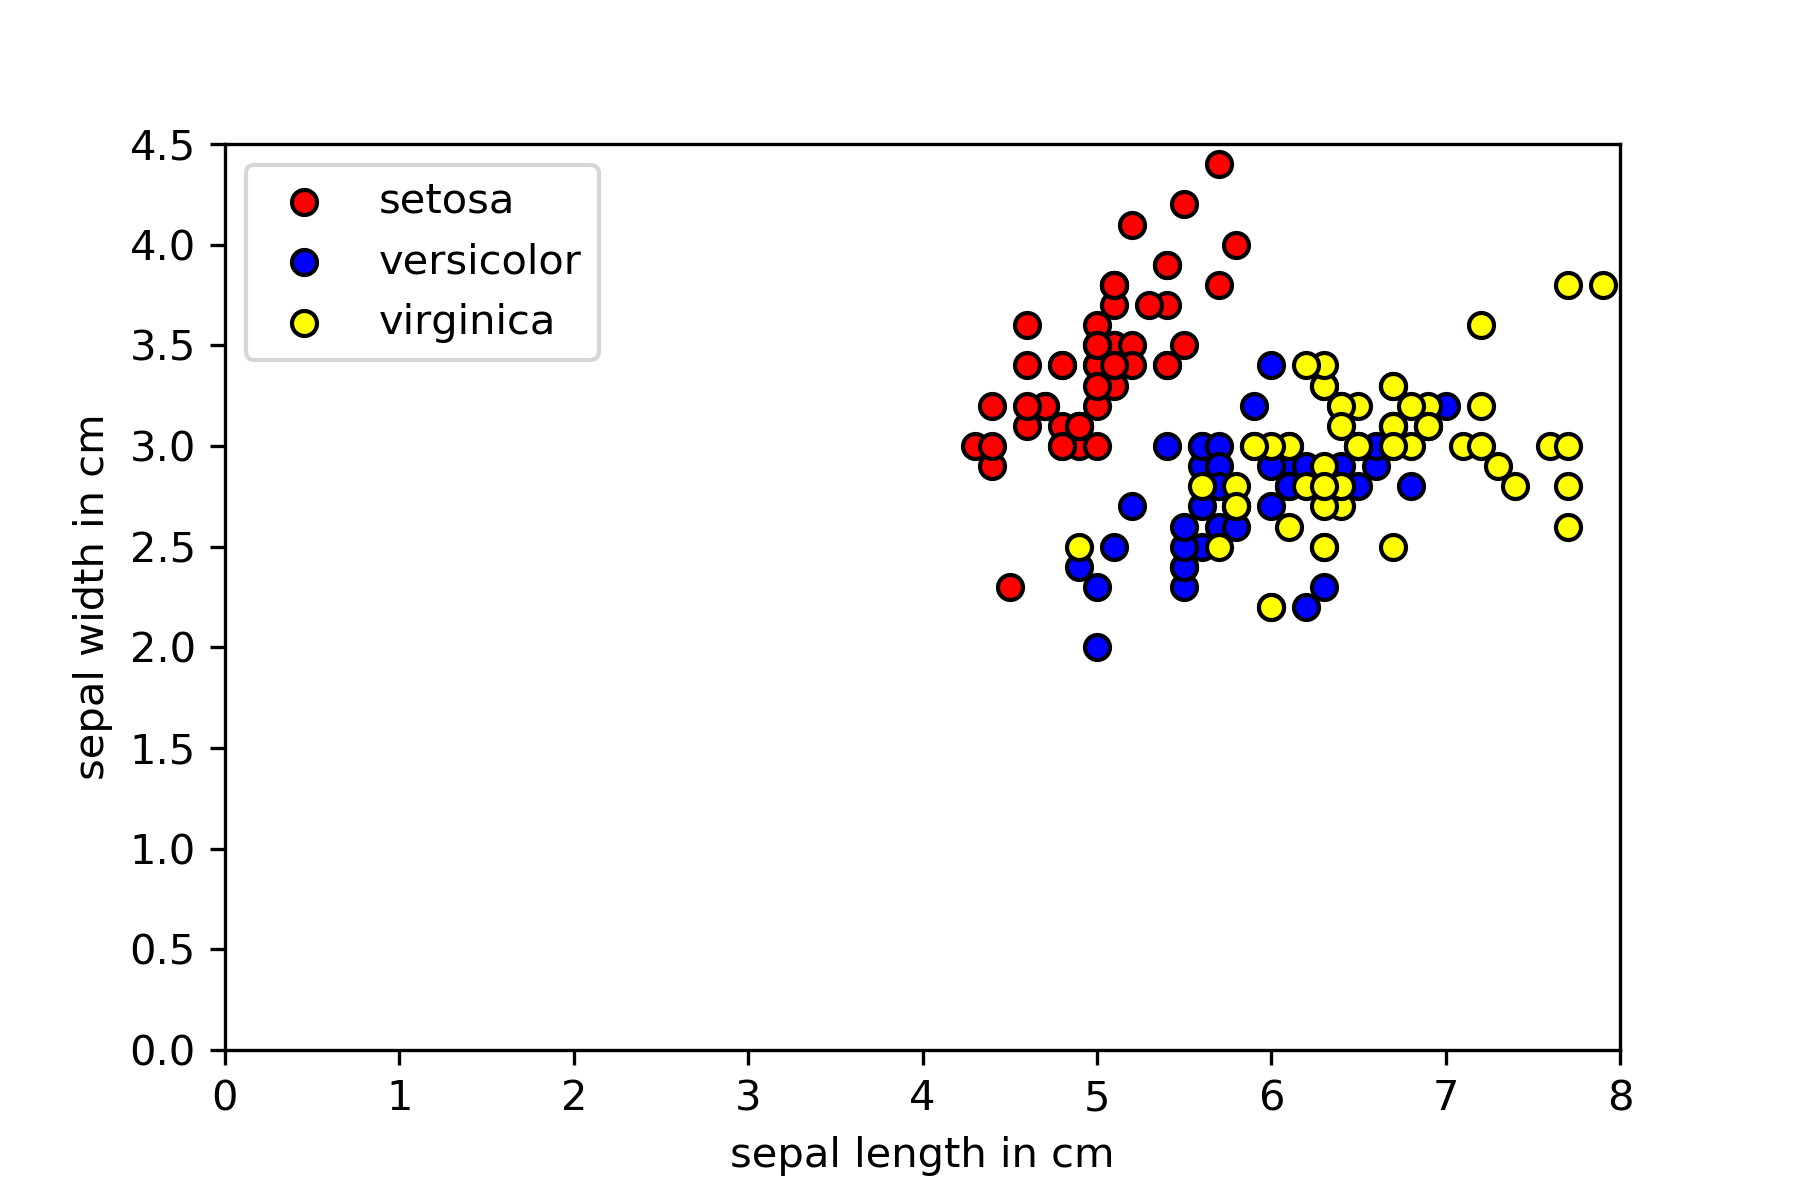
\includegraphics[width=\columnwidth]{gfx/iris/iris4features}
            \column{.6\textwidth}
            Per avere un confronto con un insieme conosciuto si sono analizzate le tre classi del noto data set Iris. 
        \end{columns}
        \vspace{.5cm}
        \begin{columns}
            \column{.3\textwidth}
            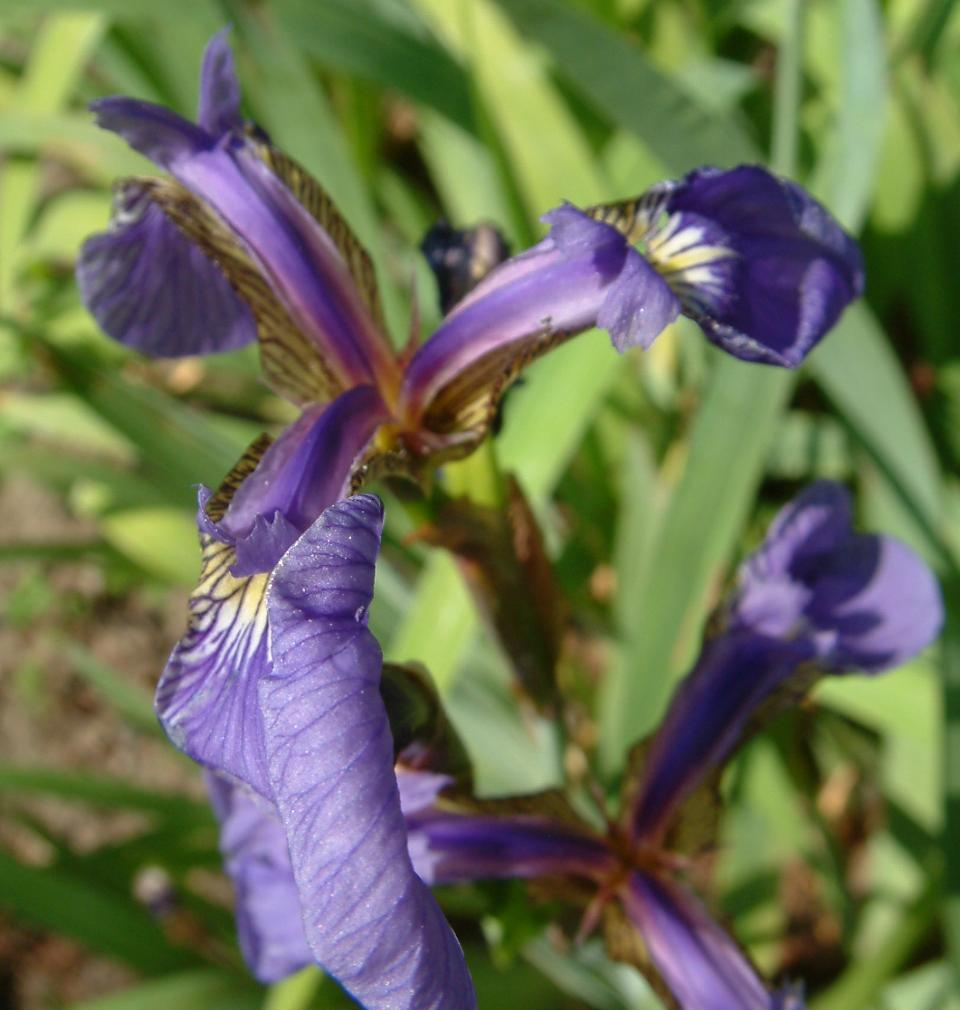
\includegraphics[width=\columnwidth]{gfx/iris/Iris_setosa.jpg}
            \column{.3\textwidth}
            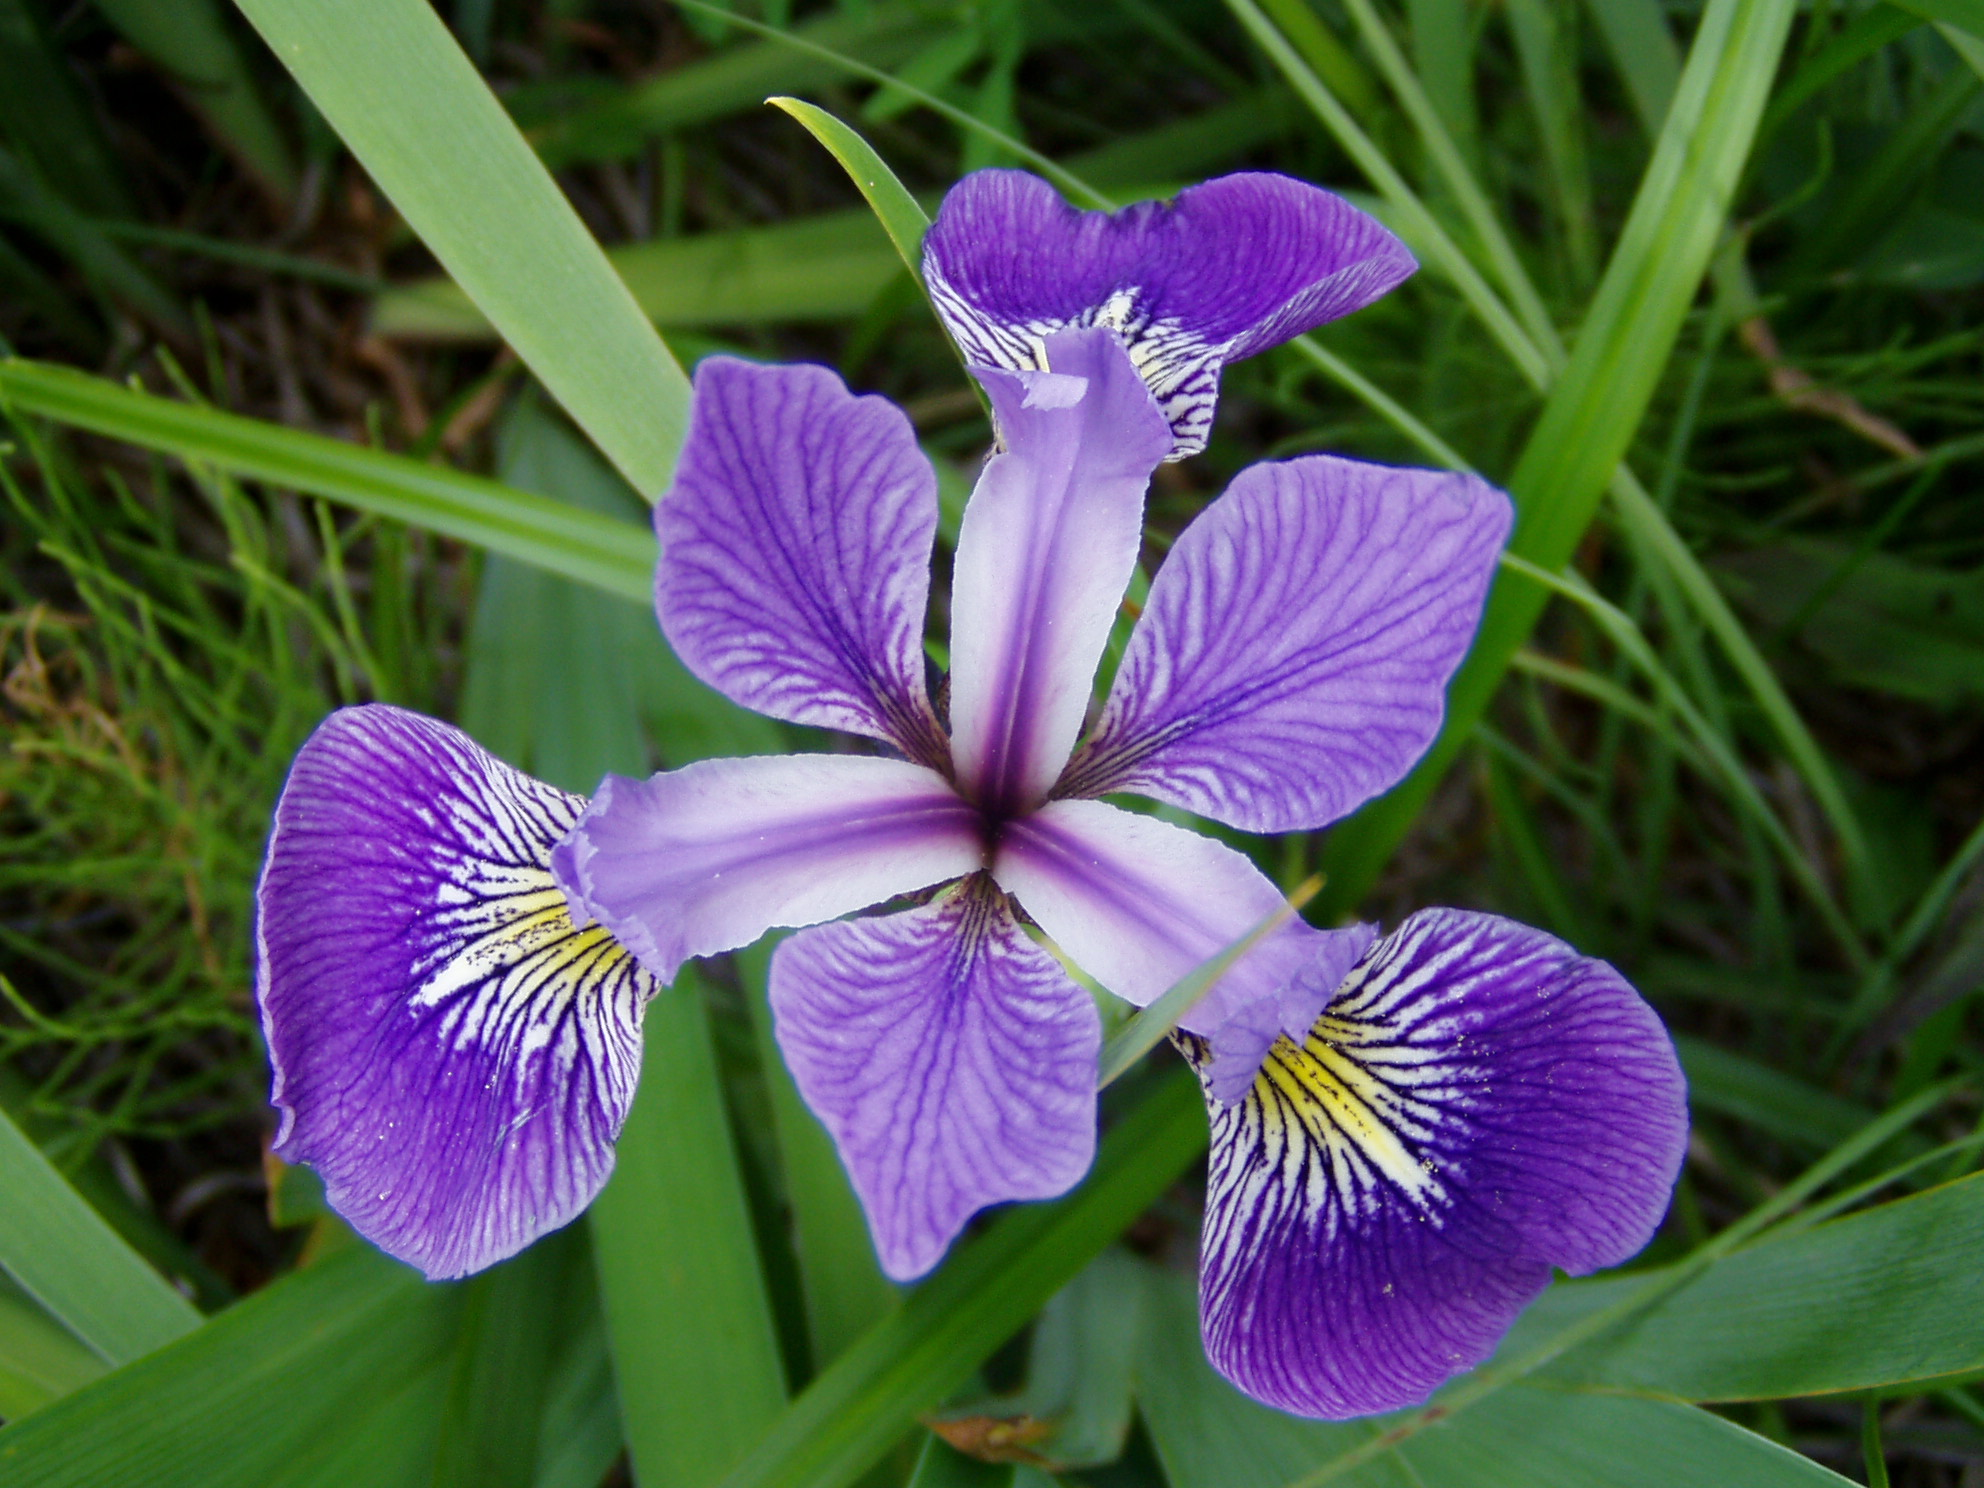
\includegraphics[width=\columnwidth]{gfx/iris/Iris_versicolor_3.jpg}
            \column{.3\textwidth}
            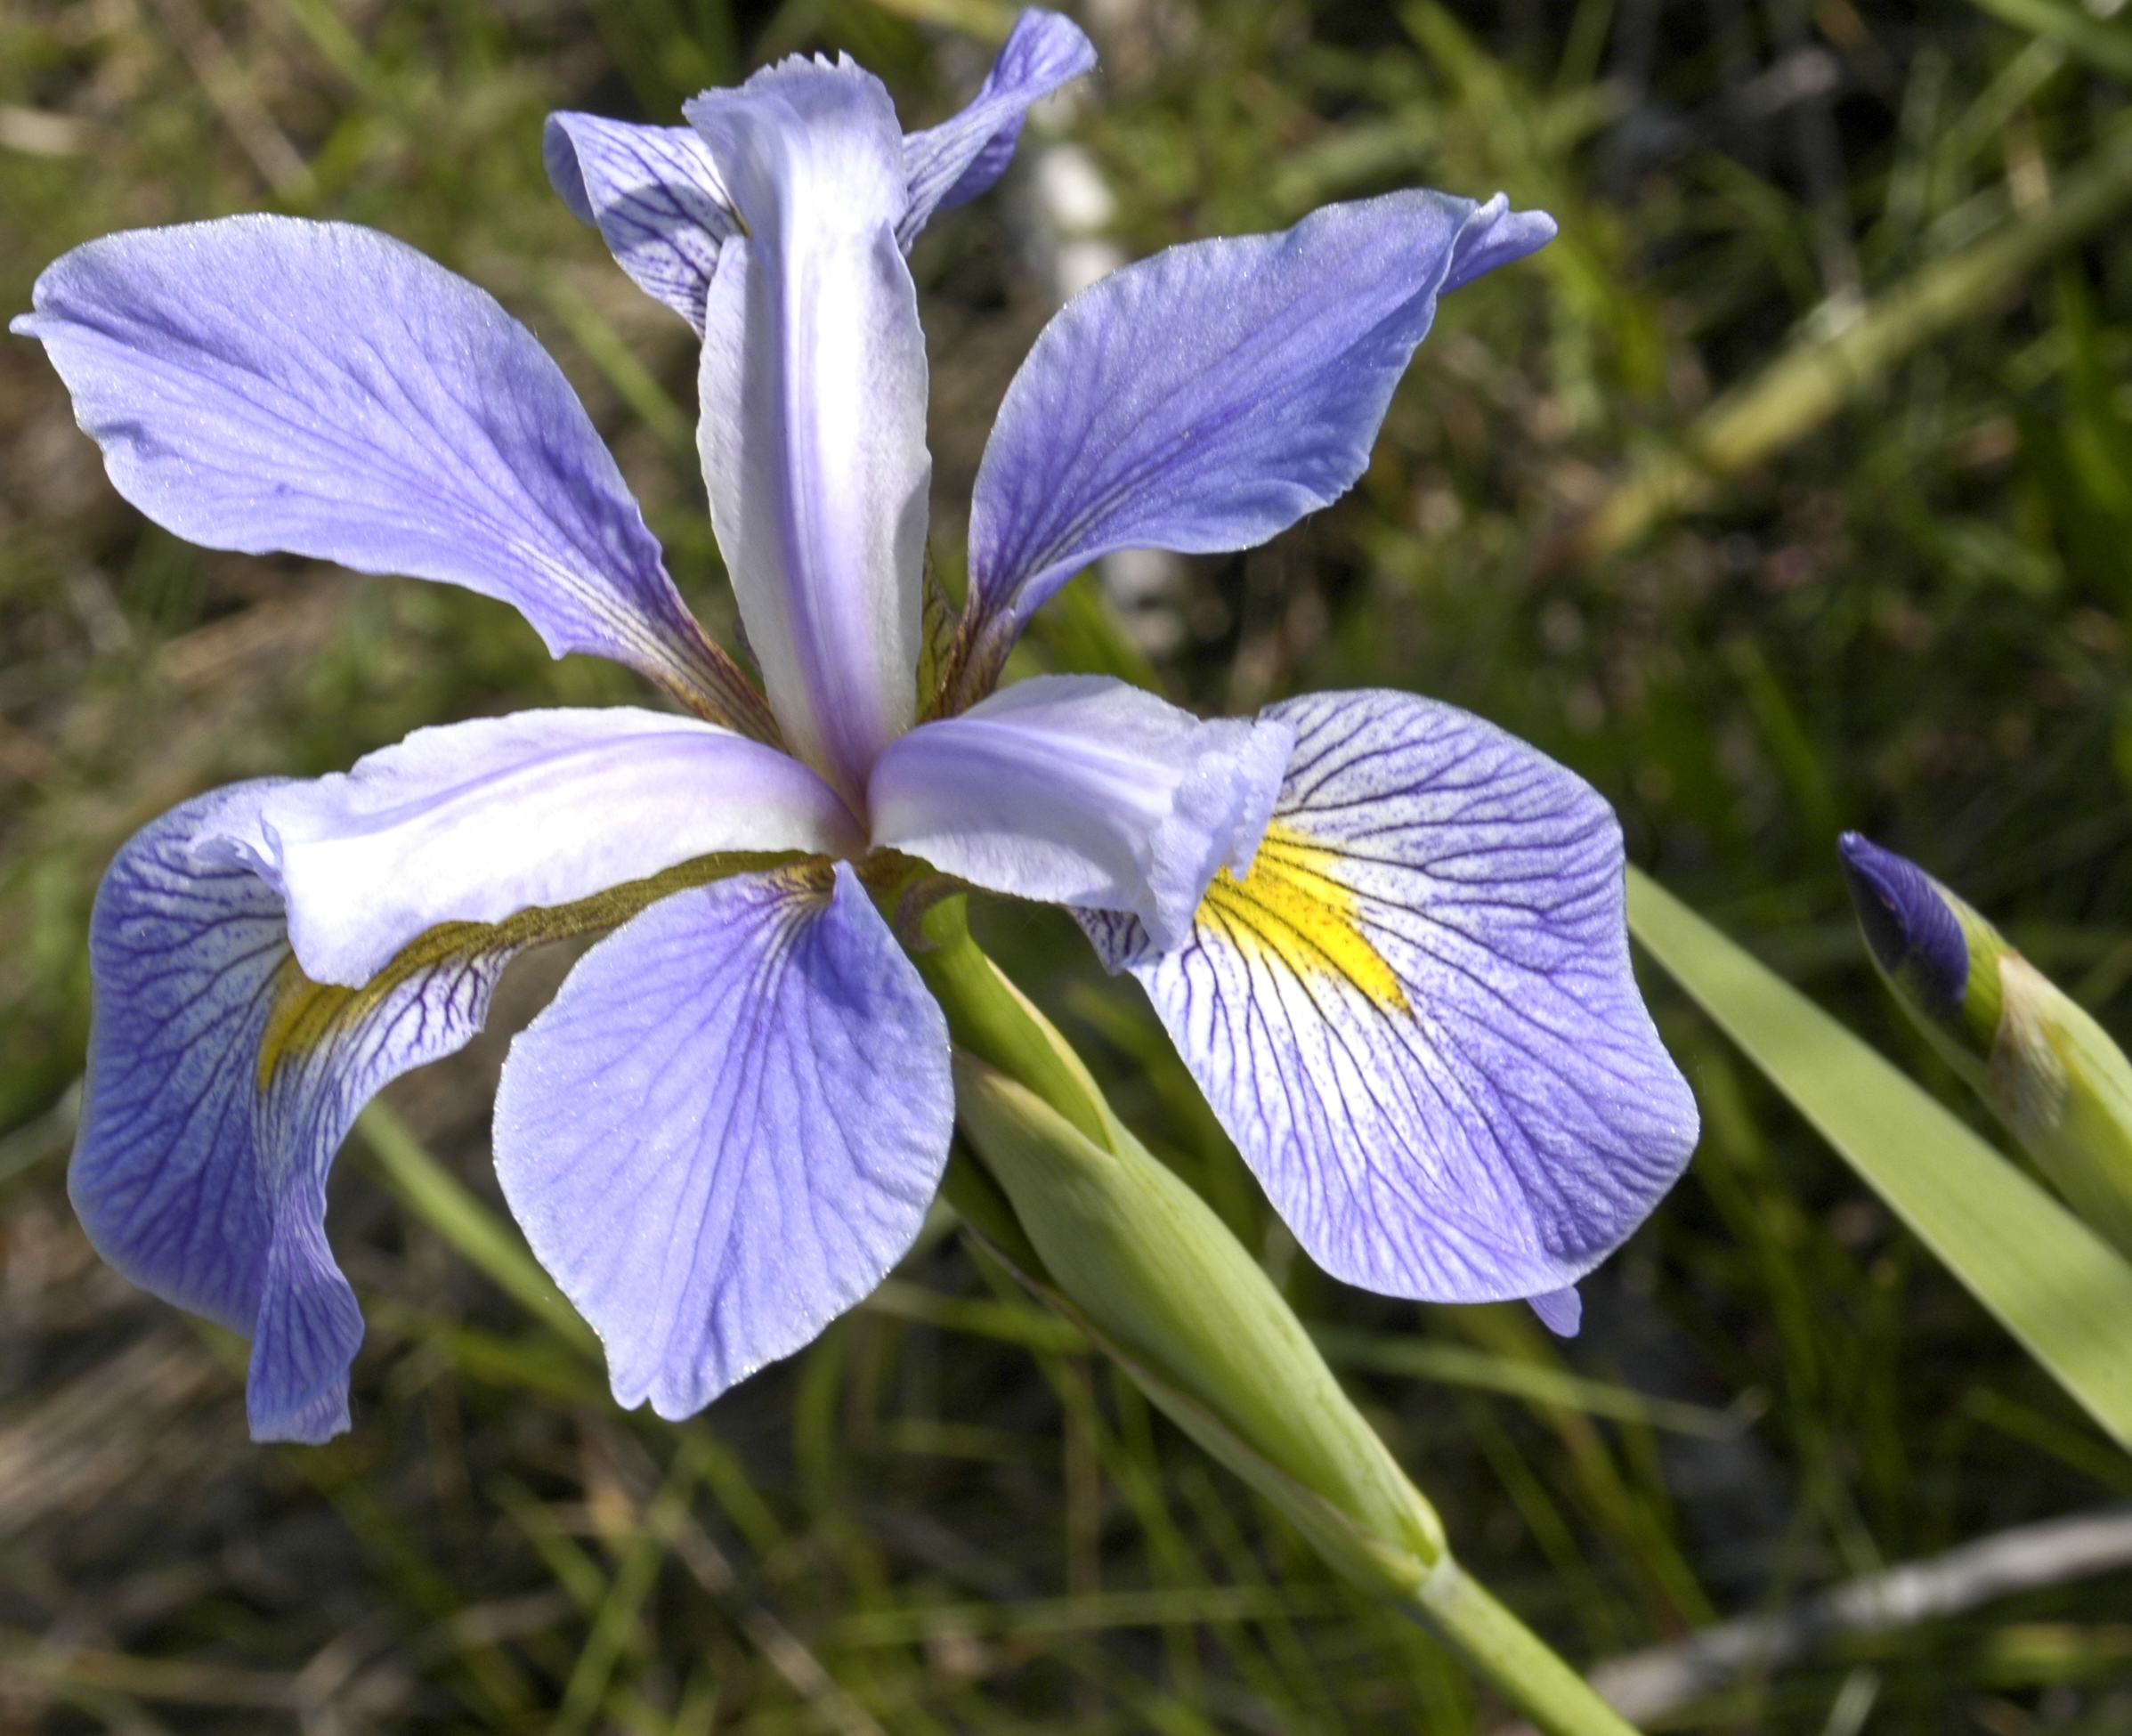
\includegraphics[width=\columnwidth]{gfx/iris/Iris_virginica.jpg}
        \end{columns}
    \end{frame}

    \begin{frame}{Preparazione dei dati}
        \begin{columns}
            \column{.4\textwidth}
            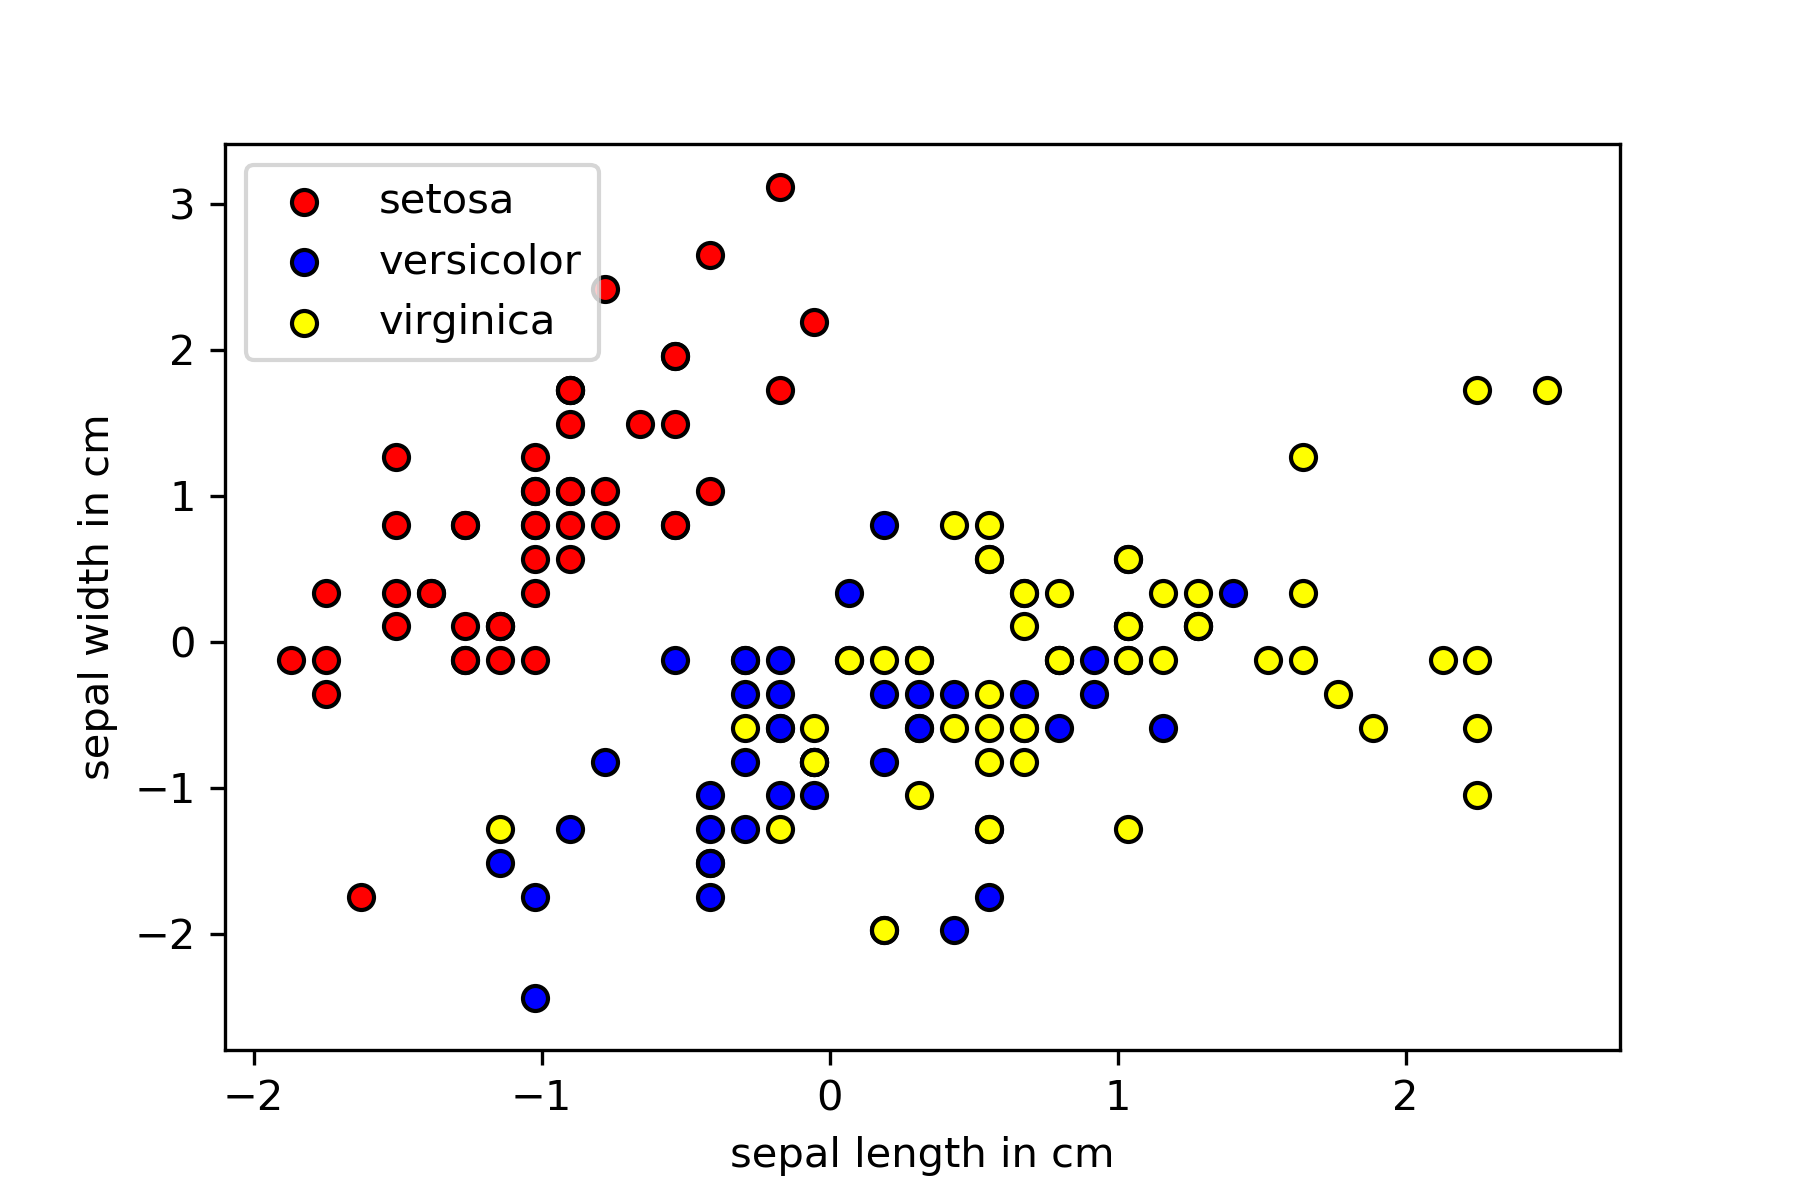
\includegraphics[width=\columnwidth]{gfx/iris/irisscaled}
            \column{.6\textwidth}
            Si è centrato nell'origine e scalato i dati in modo che avessero varianza unitaria. 

            Successivamente il data set è stato normalizzato per ragioni di compatibilità con l'algoritmo. 
        \end{columns}

        \vspace{.5cm}

        \begin{columns}
            \column{.5\textwidth}
            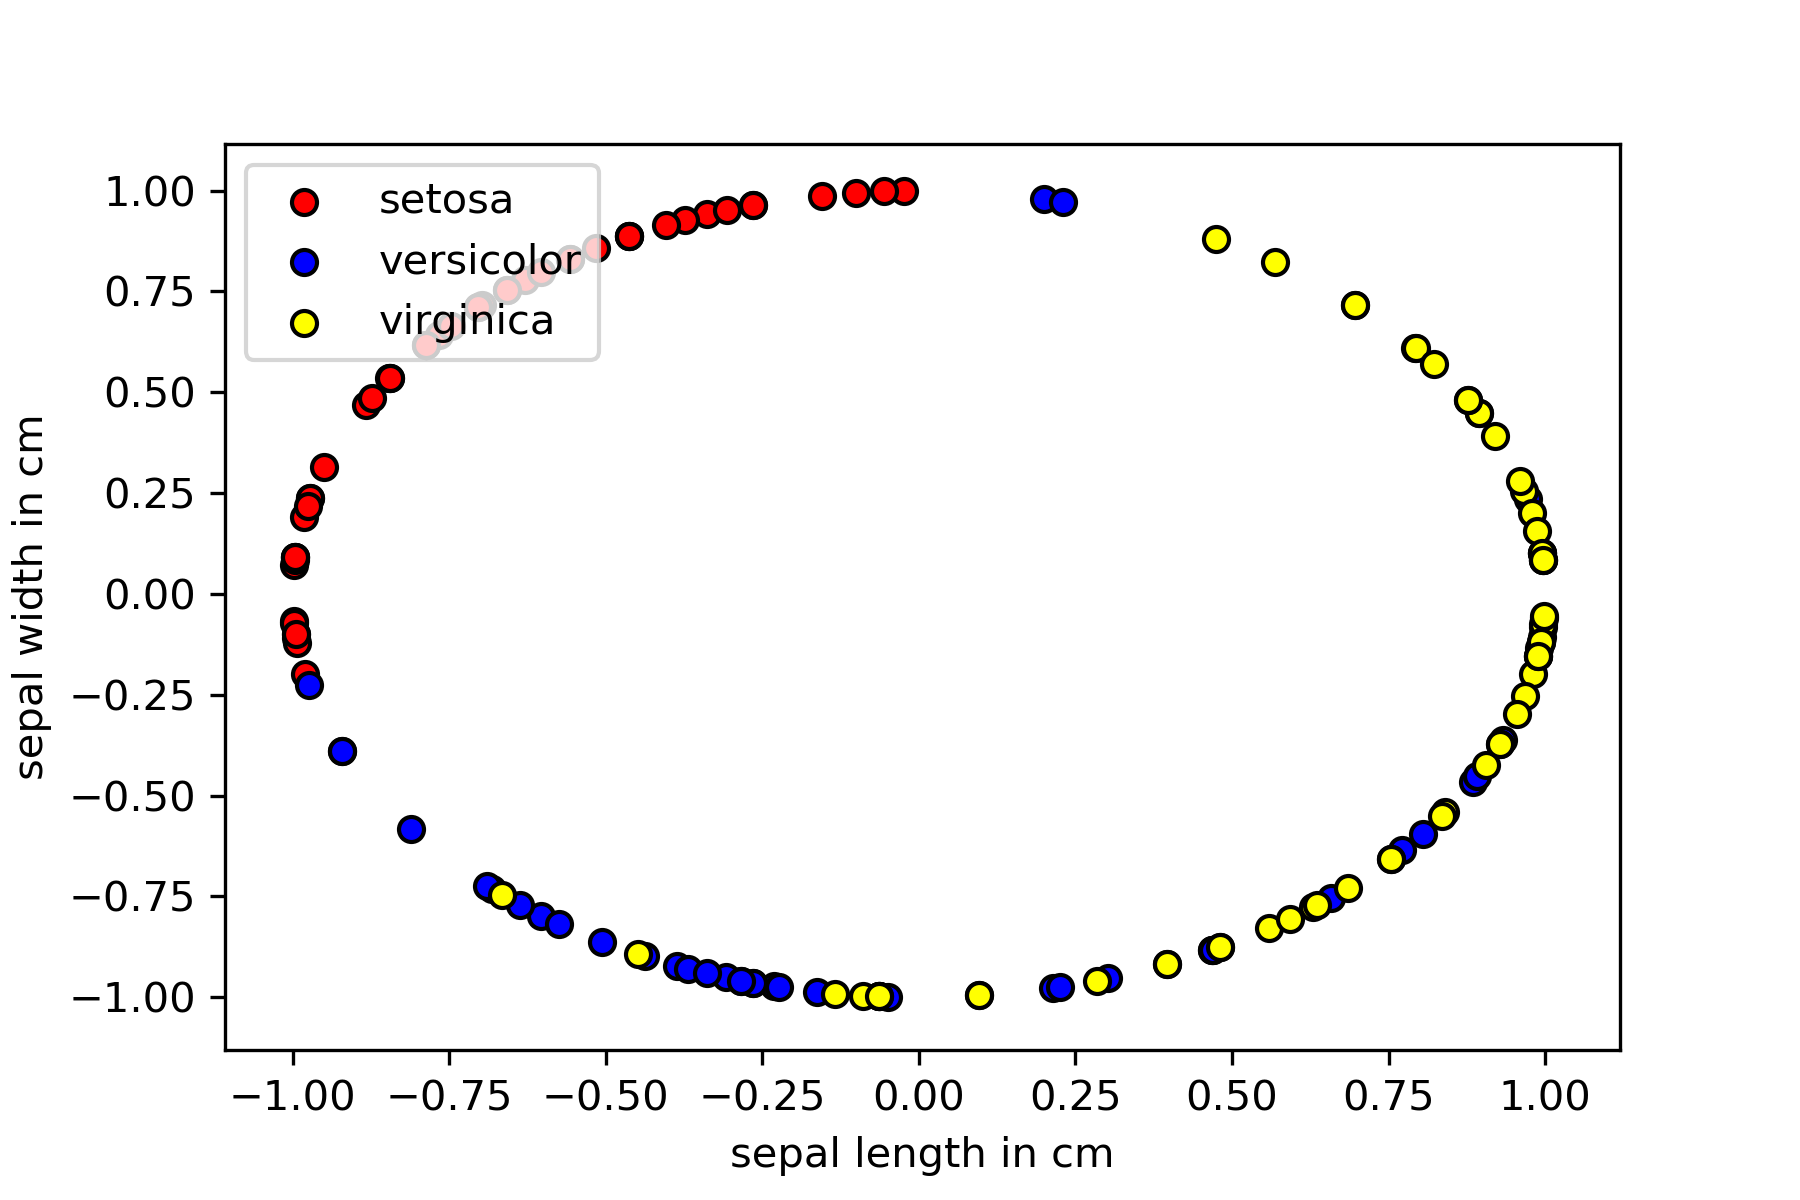
\includegraphics[width=\columnwidth]{gfx/iris/irisnormalized}
            \column{.5\textwidth}
            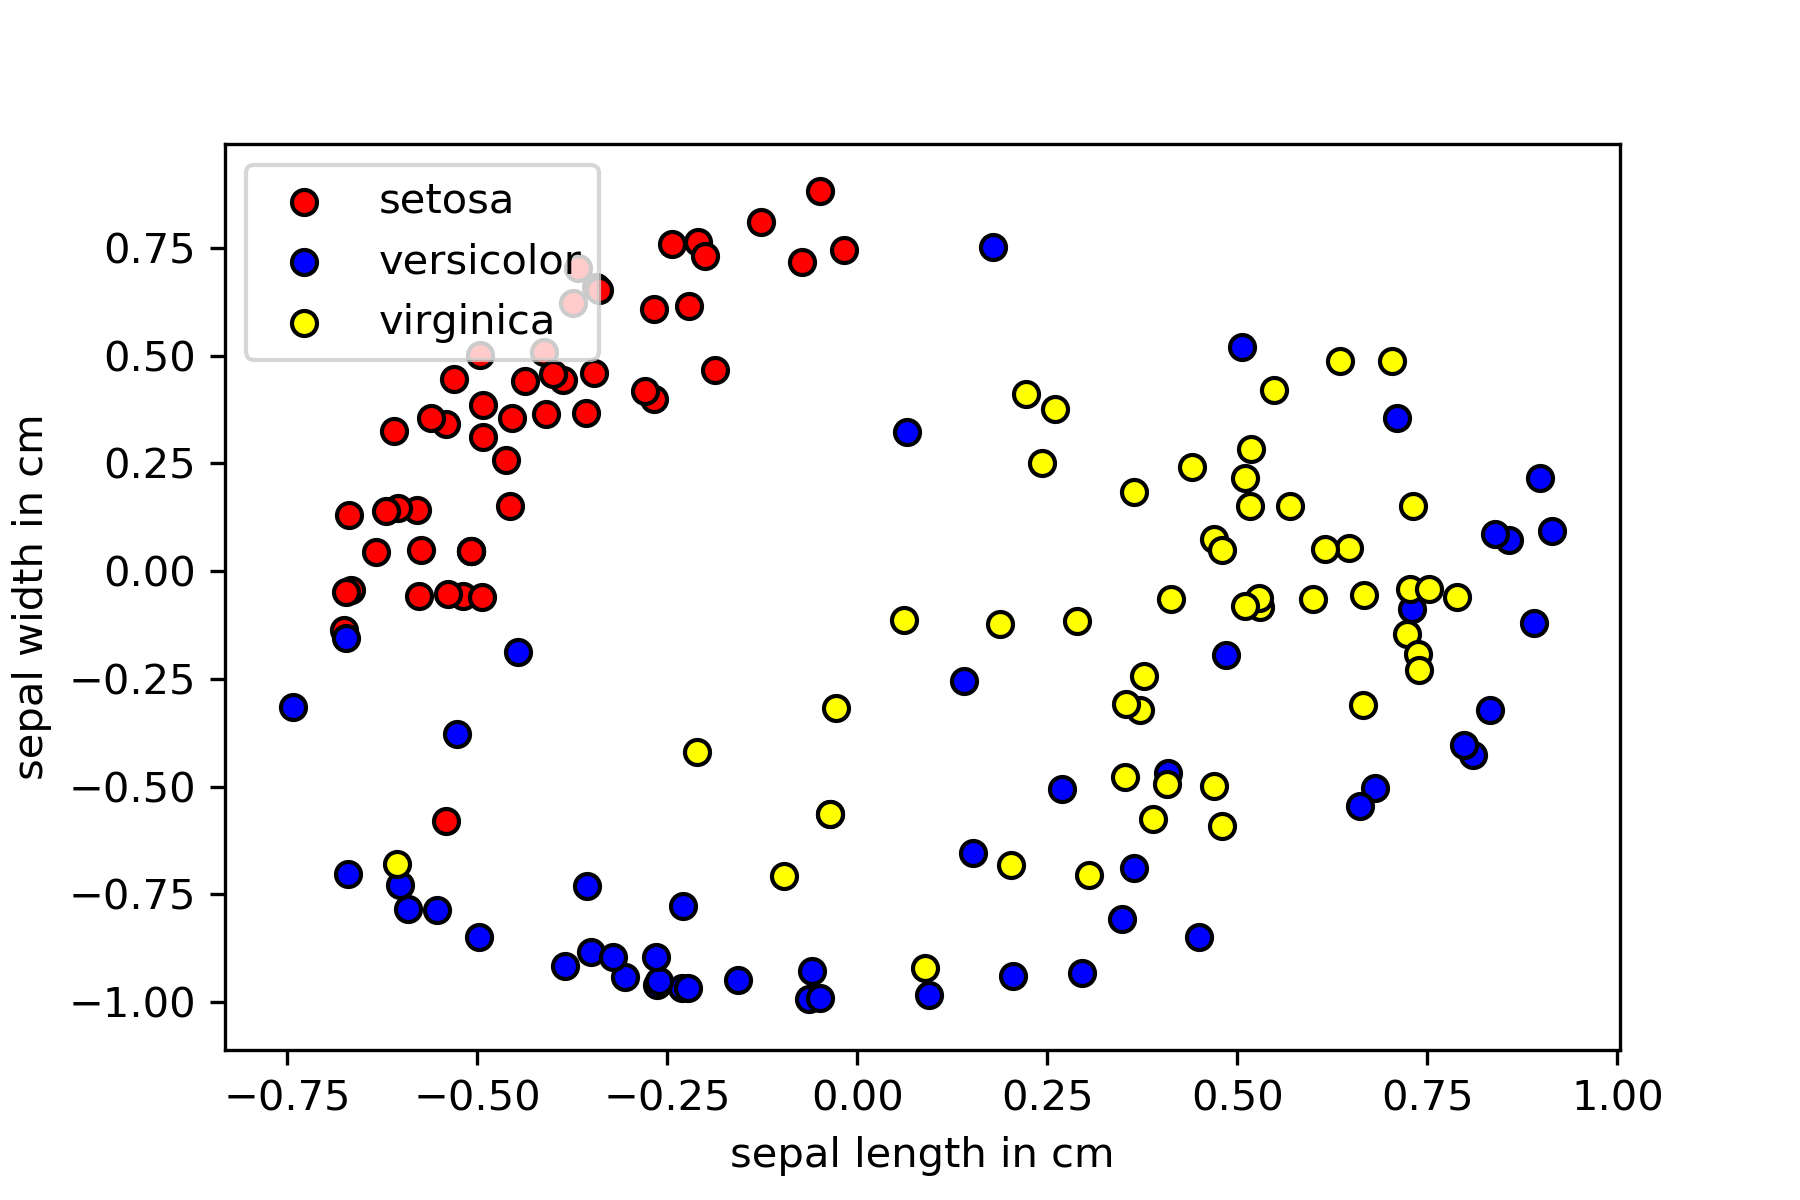
\includegraphics[width=\columnwidth]{gfx/iris/iris4normalized}
        \end{columns}
    \end{frame}

    \begin{frame}{Classificazione binaria (setosa vs. versicolor)}
        \begin{columns}
            \column{.5\textwidth}
            \begin{figure}[h]
                \centering
                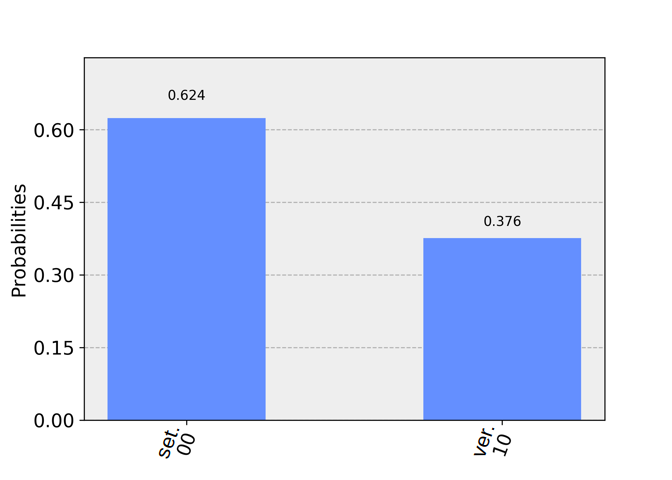
\includegraphics[width=\textwidth]{gfx/misura_setosa_filtrata_20191015_1145.png}
                \caption{Simulazione su setosa}
                \label{fig:simulazione.setosa}
            \end{figure}
            \column{.5\textwidth}
            \begin{figure}[h]
                \centering
                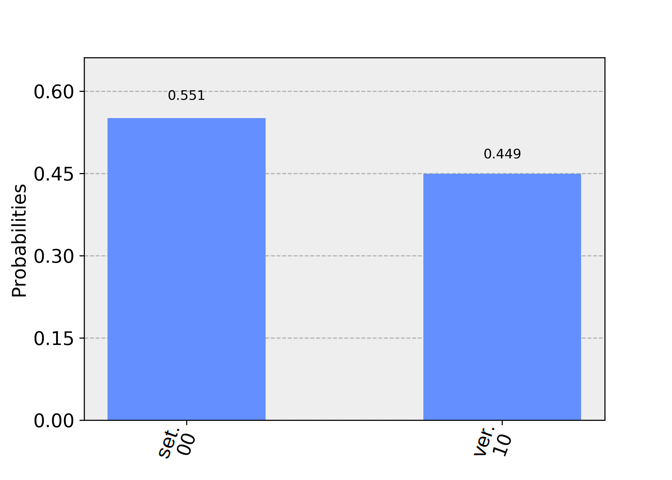
\includegraphics[width=\textwidth]{gfx/misura_setosa_sperimentale.png}
                \caption{Esecuzione reale su setosa}
                \label{fig:esecuzione.setosa}
            \end{figure}
        \end{columns}
    \end{frame}

    \begin{frame}{Classificazione multiclasse (setosa vs. versicolor vs. virginica)}
        % Classificazione setosa vs. versicolor vs. virginica dal data set Iris
        \begin{columns}
            \column{.5\textwidth}
            \begin{figure}[h]
                \centering
                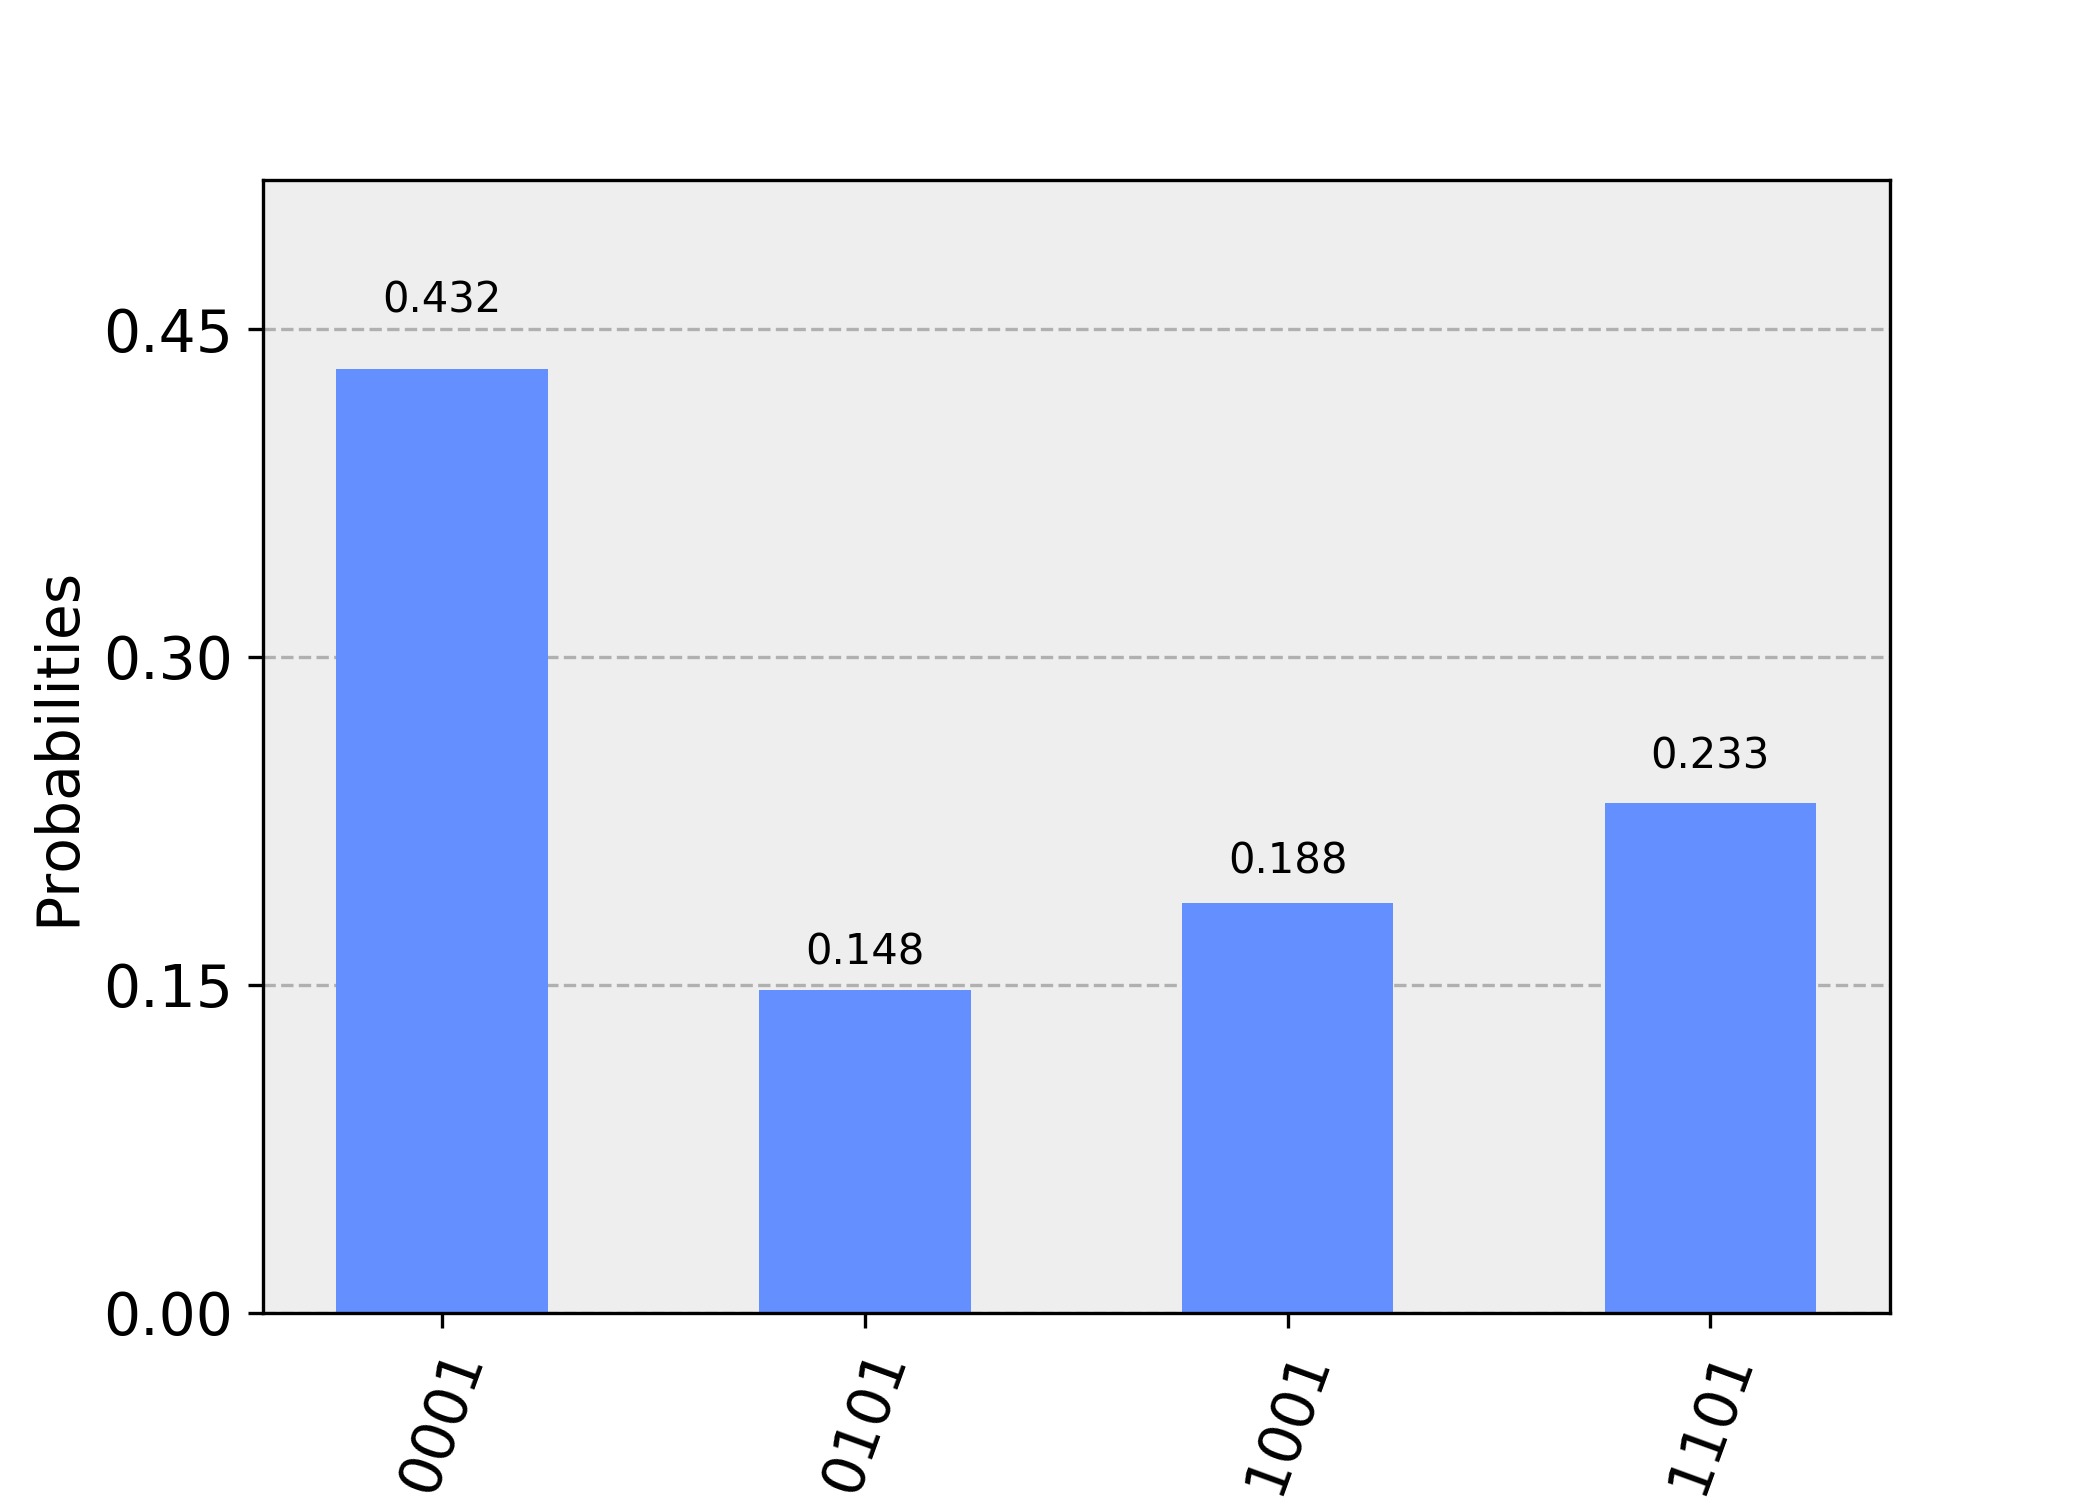
\includegraphics[width=\textwidth]{gfx/setosa_simulato_multiclasse.png}
                \caption{Simulazione su setosa}
                \label{fig:simulazione.multi.setosa}
            \end{figure}
            \column{.5\textwidth}
            \begin{figure}[h]
                \centering
                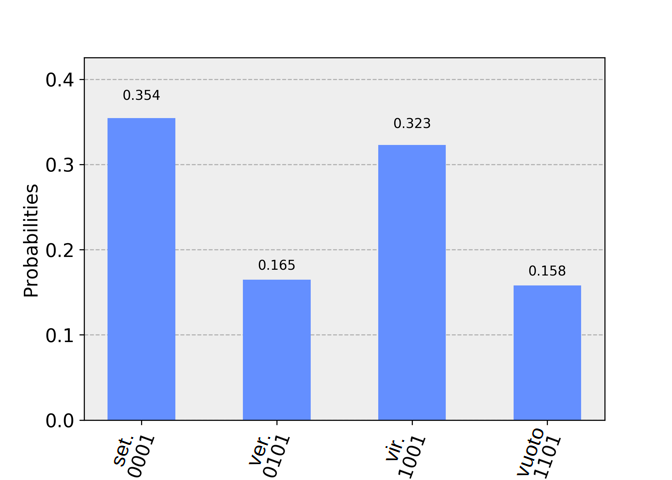
\includegraphics[width=\textwidth]{gfx/setosa_reale_20190913:1716.png}
                \caption{Esecuzione reale su setosa}
                \label{fig:esecuzione.multi.setosa}
            \end{figure}
        \end{columns}
    \end{frame}

    \begin{frame}{Classificazione multiclasse}
        \begin{columns}
            \column{.45\textwidth}
            \rotatebox{90}{Sim. versicolor}
            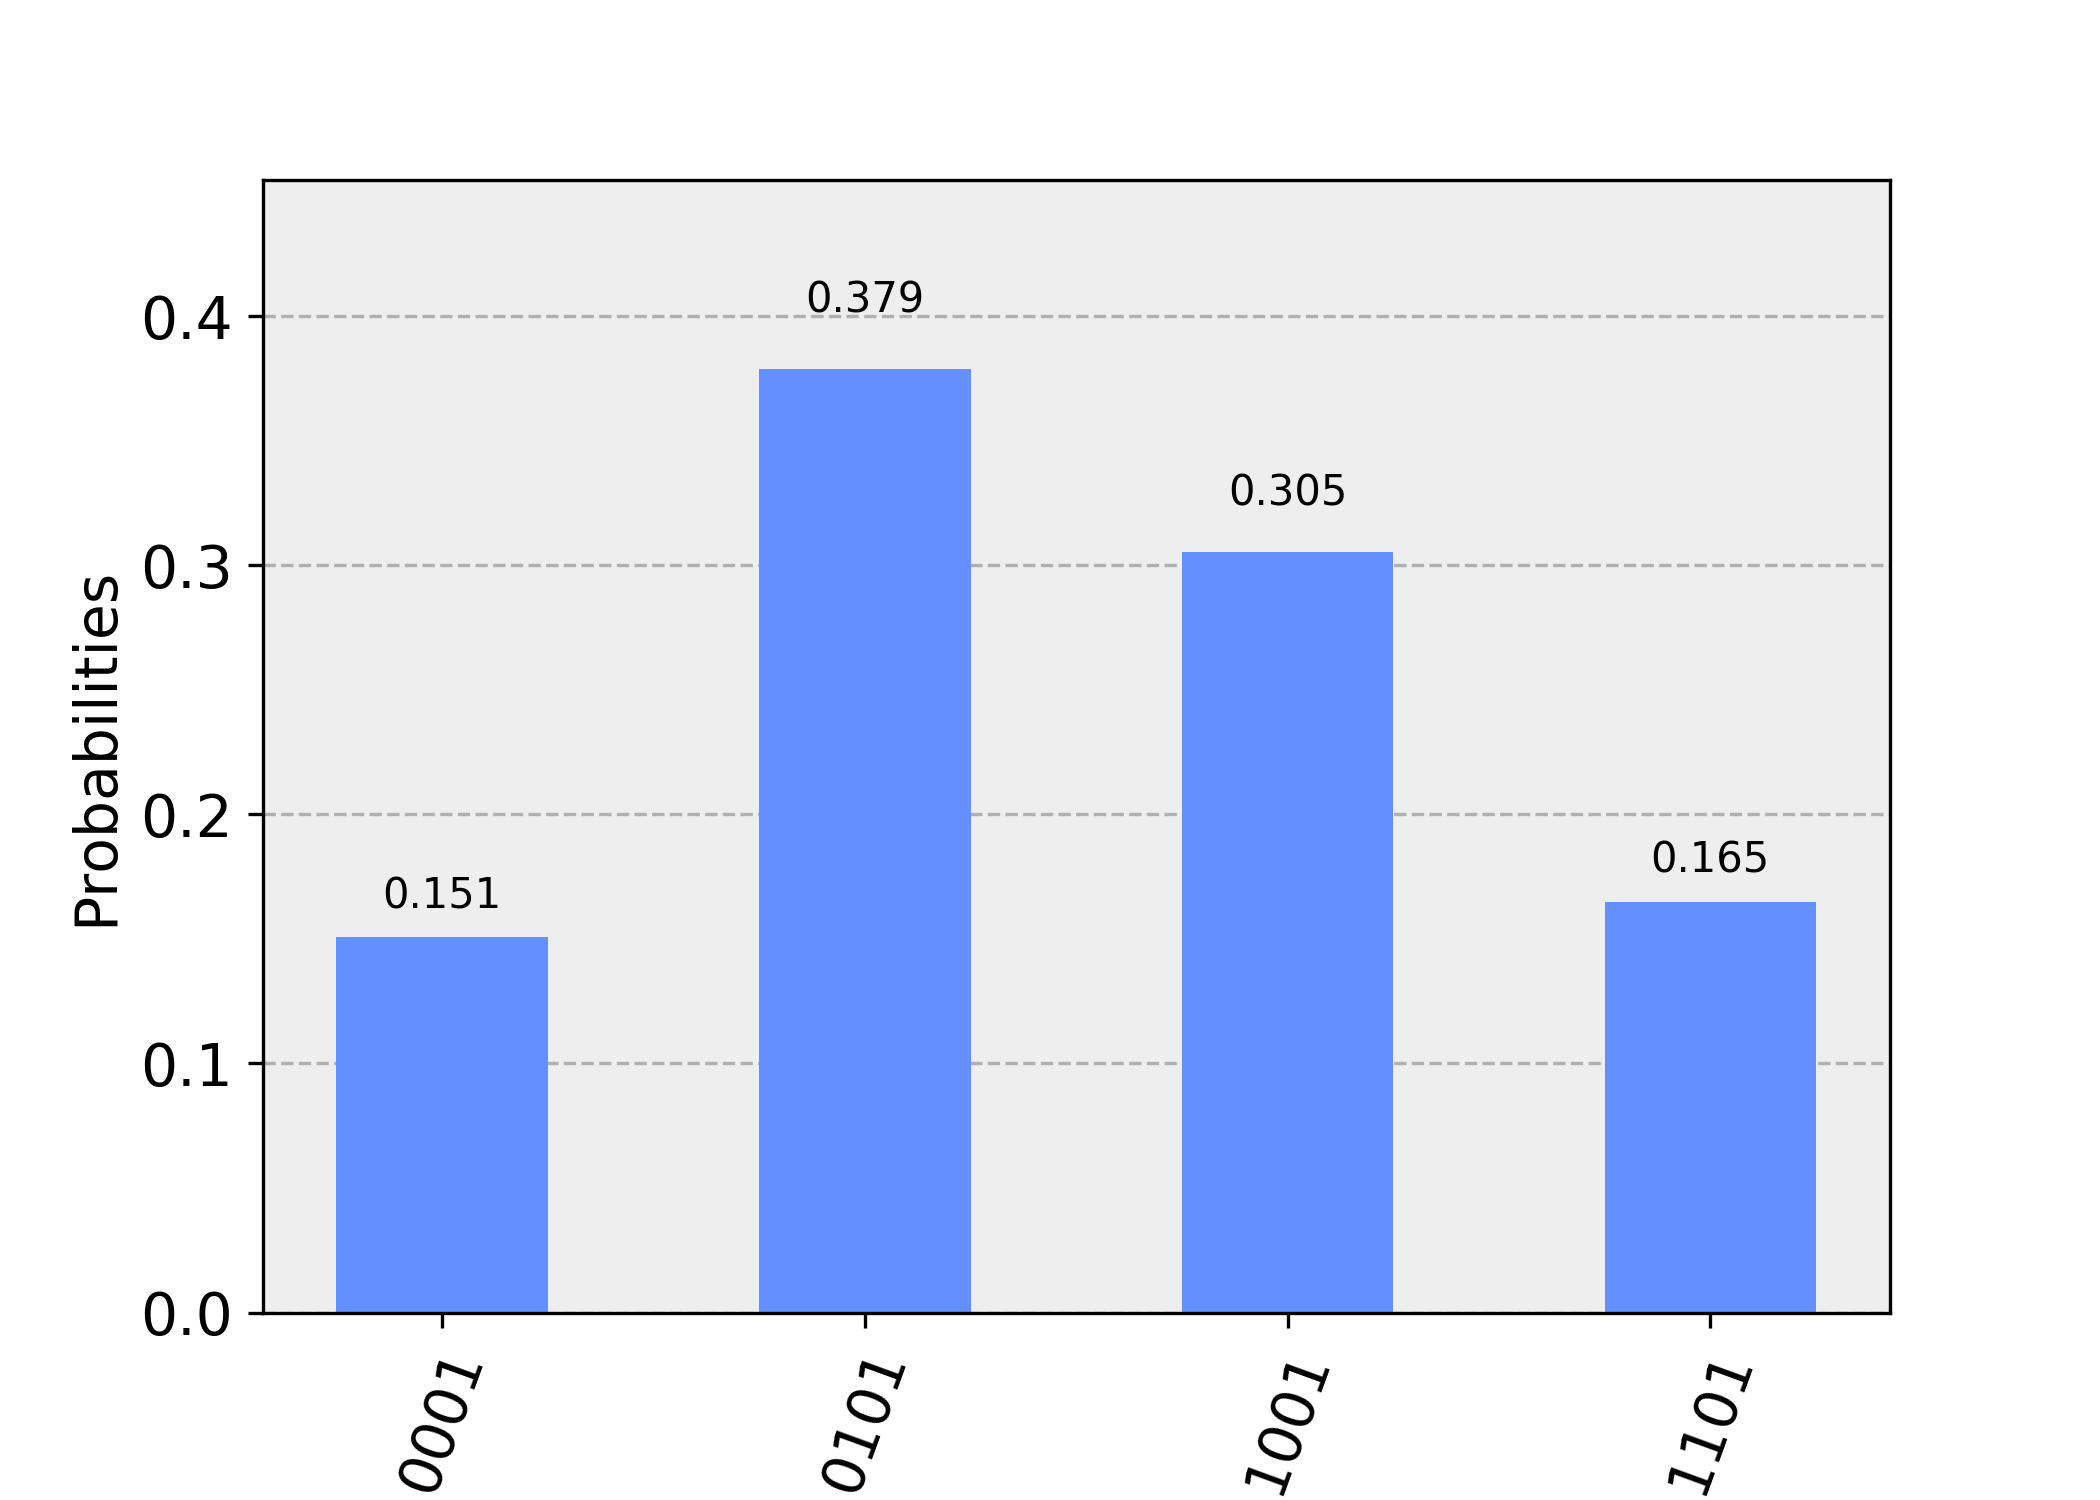
\includegraphics[width=.9\linewidth]{gfx/multiclass_versicolor}
            \column{.45\textwidth}
            \rotatebox{90}{Sim. virginica}
            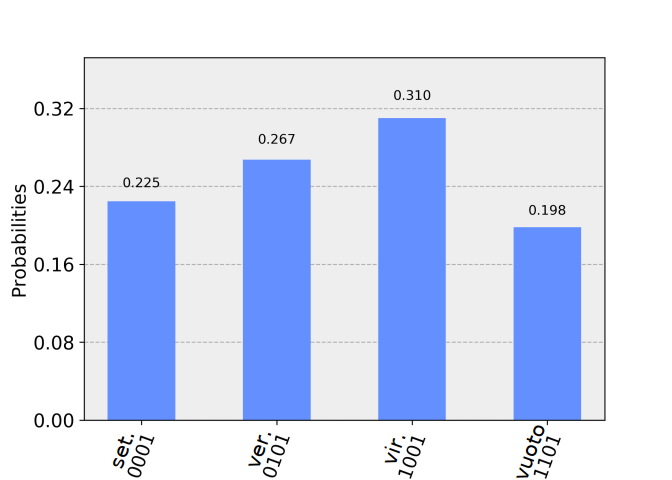
\includegraphics[width=.9\linewidth]{gfx/multiclass_virginica}
        \end{columns}
        \begin{columns}
            \column{.45\textwidth}
            \rotatebox{90}{Reale versicolor}
            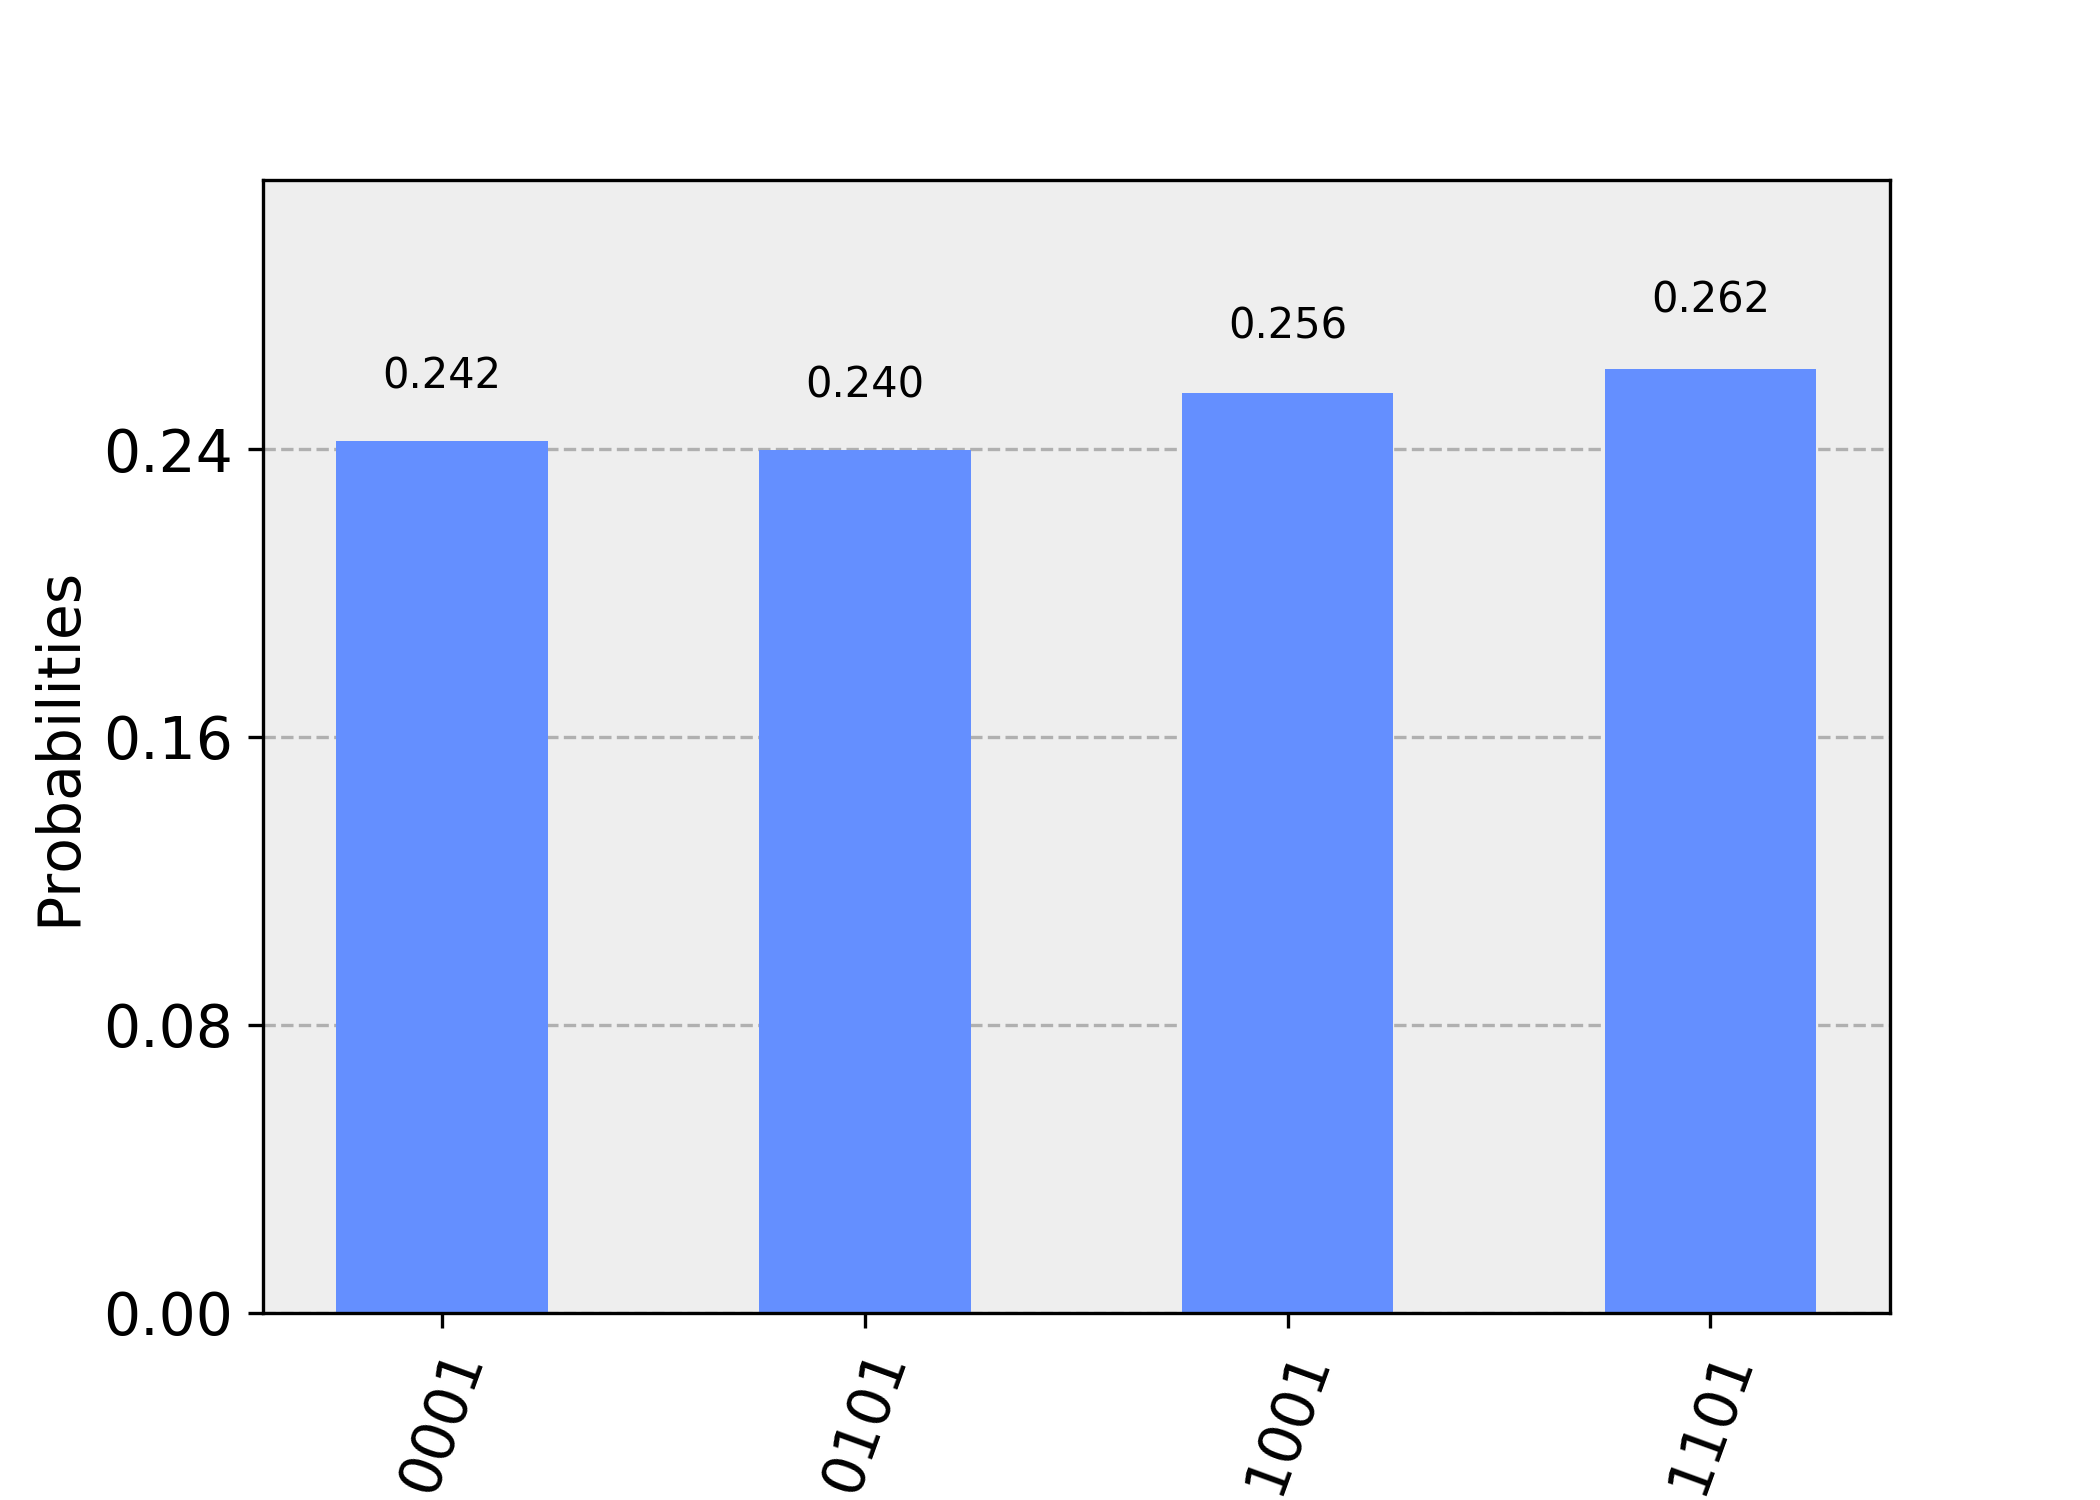
\includegraphics[width=.9\linewidth]{gfx/versicolor_reale_20191015_1506.png}
            \column{.45\textwidth}
            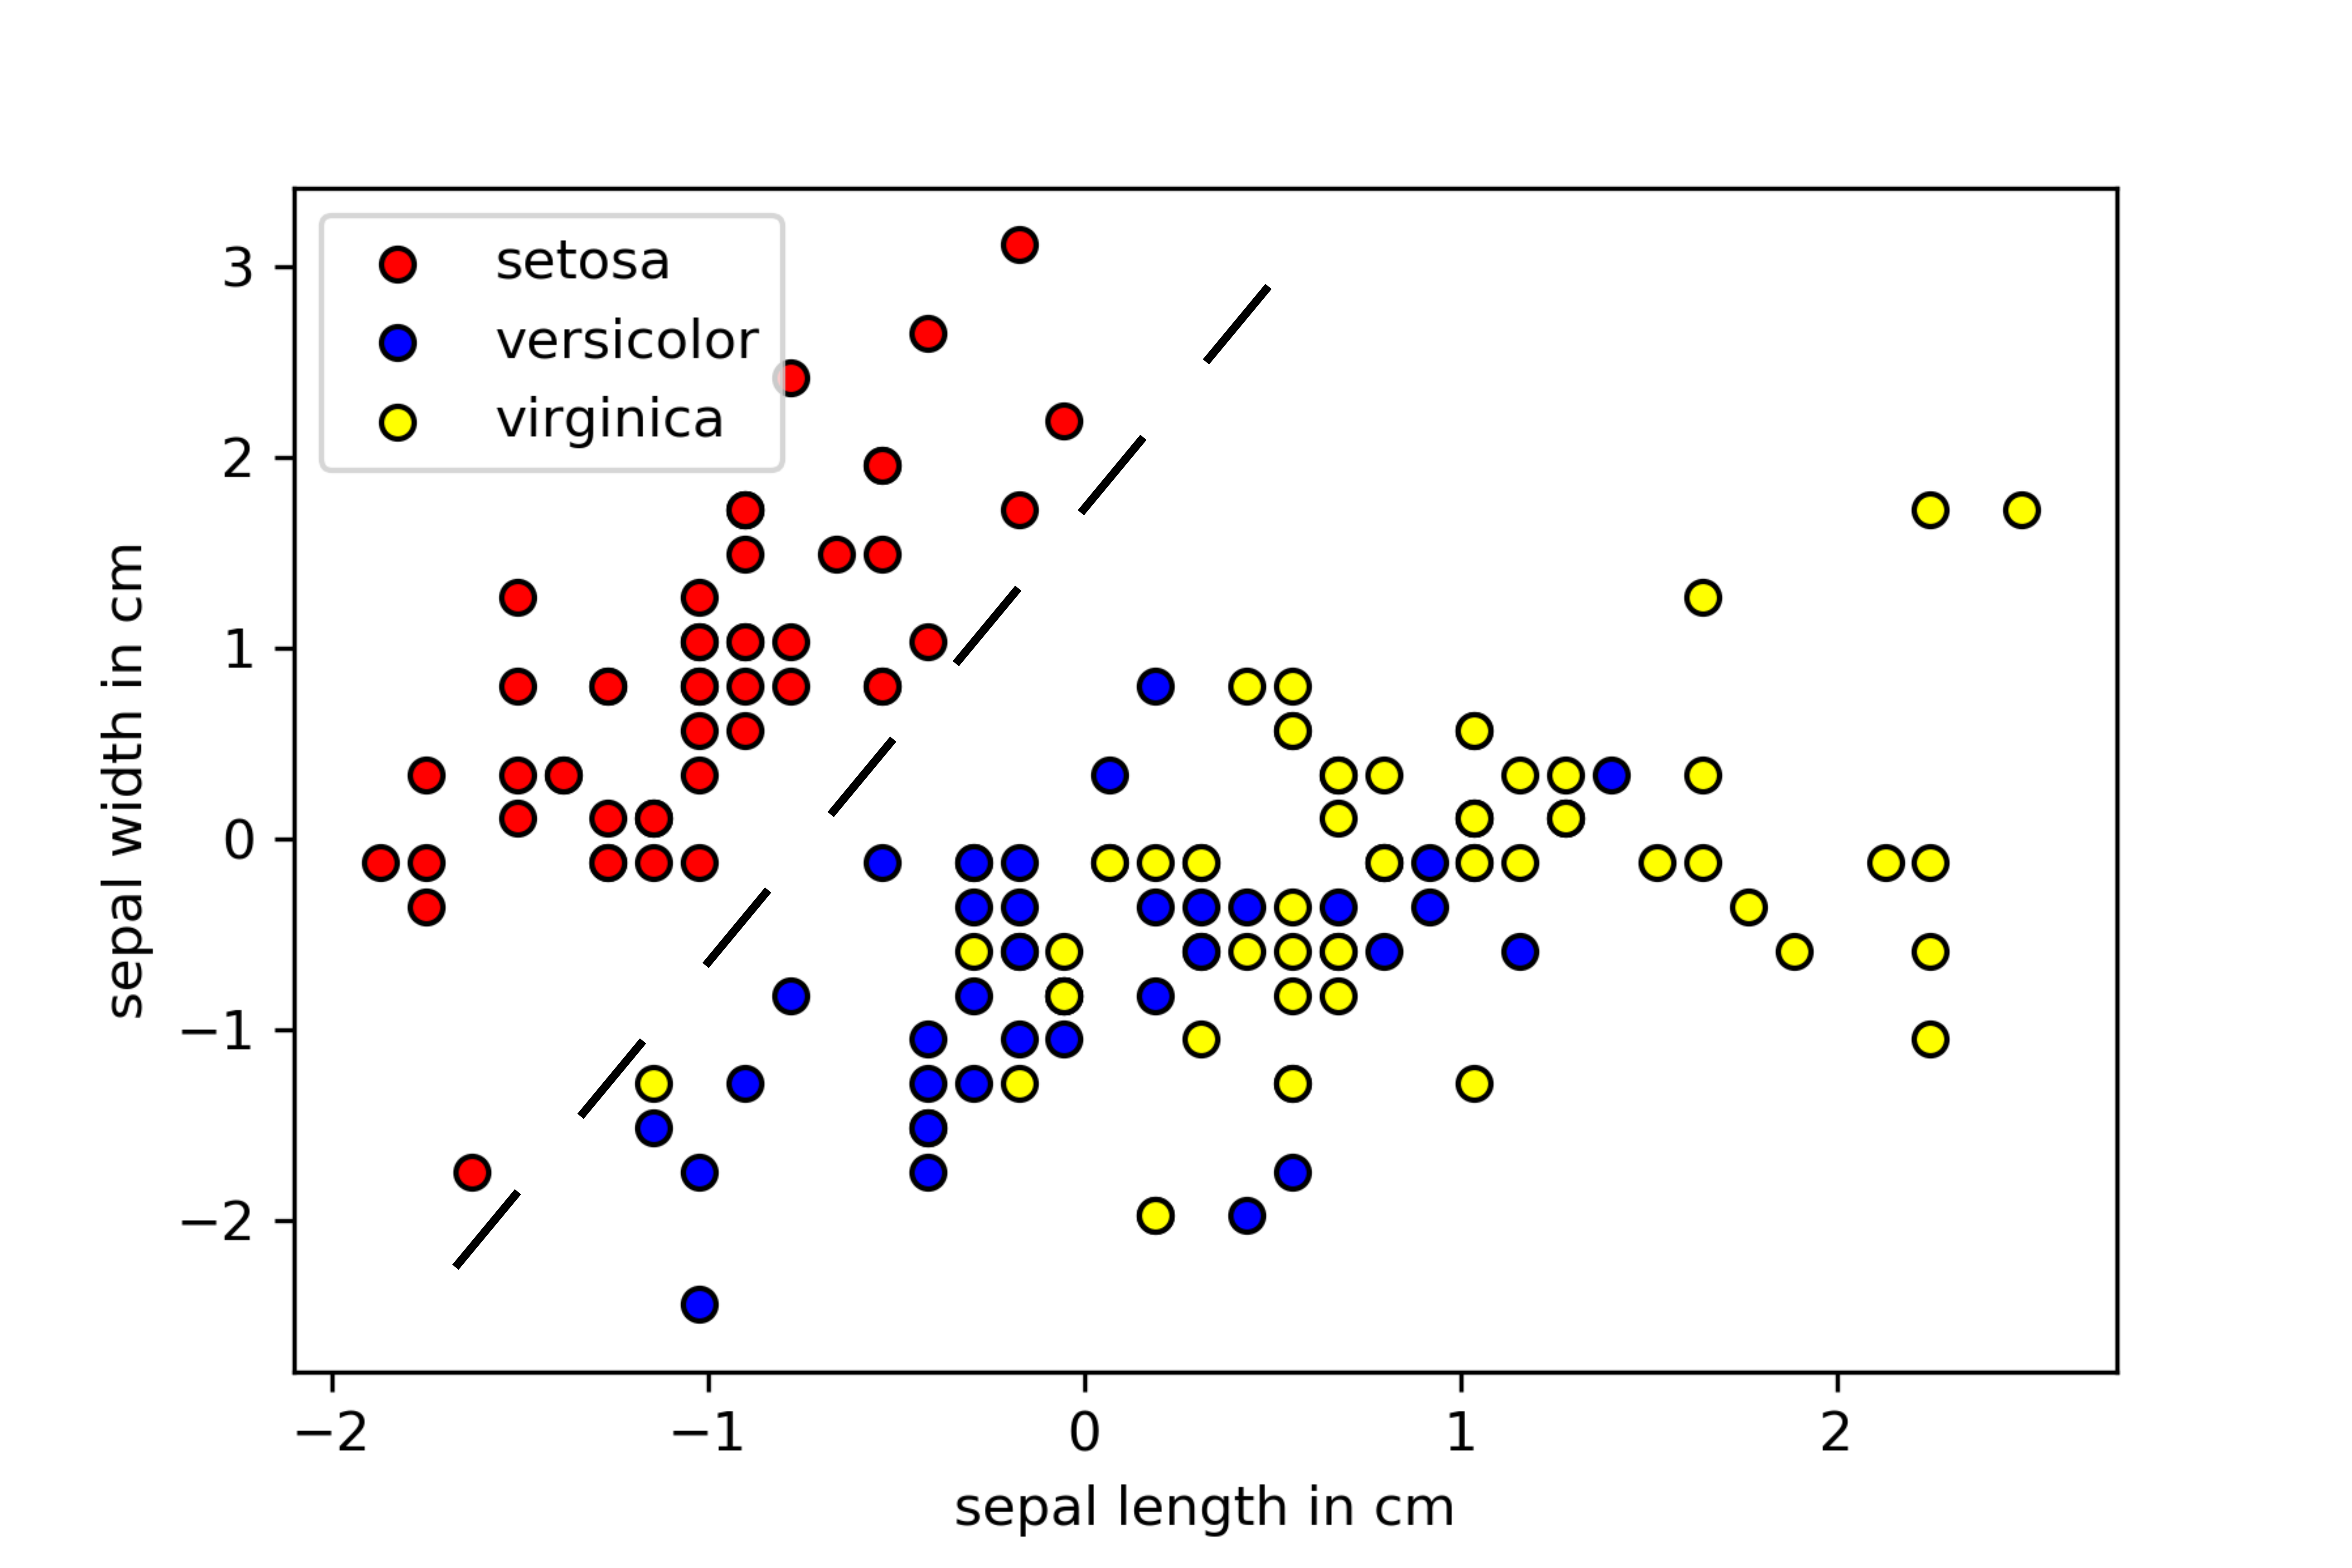
\includegraphics[width=\columnwidth]{gfx/iris/irisscaled_separation.png}
        \end{columns}
        
        % Nota importante: gli elementi delle classi versicolor e virginica non sono linearmente separabili. 

        % Pertanto qualsiasi algoritmo basato sulla distanza non è efficiente nel distinguere tra le due classi 
        % senza ottimizzazione dei dati, sia esso classico o quantistico. 
    \end{frame}

    \begin{frame}{Efficienza di esecuzione}
        \begin{columns}
            \column{.4\textwidth}
            \begin{table}[h!]
                \centering
                \begin{tabular}{c c}
                    classe & esiti positivi\\
                    \hline
                    verde & 100\%\\
                    blu & 88,9\%\\
                    nero & 100\%\\
                    giallo & 100\%
                \end{tabular}
                \caption{Risultati positivi per simulazione su cluster con otto vettori di training}
            \end{table}    
            \column{.6\textwidth}
            \begin{table}[h!]
                \centering
                \begin{tabular}{c c c c}
                    classe & m=3 & $m=5$ & $m=7$ \\ 
                    \hline
                    setosa & 100\% & 100\% & 100\%\\ 
                    versicolor & 30\% & 50\% & 80\%\\ 
                    virginica & 60\% & 90\% & 90\%
                \end{tabular}
                \caption{Risultati positivi per simulazione su Iris con $2^m$ vettori di training}
                \label{table:misure}
            \end{table}
        \end{columns}
        Il tasso di errore stimato sul data set Iris per il classificatore KNN classico è del 4,67\%.\footnote{https://www.mathworks.com/help/bioinfo/ref/classperf.html}
    \end{frame}

    \section{Conclusione}

    \begin{frame}{Riassunto}
        \begin{itemize}
            \item L'elaborazione quantistica è nella frontiera dei supercomputer e ha il potenziale di accelerare gli algoritmi di machine learning classico
            \item È stata riprodotta un'implementazione di algoritmo KNN quantistico di classificazione binaria su hardware di piccola e media scala e 
            se ne è esteso il funzionamento grazie alla procedura di costruzione di stati arbitrari FF-QRAM in modo da renderlo multiclasse. 
            \item La complessità algoritmica è stimata come $\mathcal{O}(MNr)$, usando $\mathcal{O}(\log_2(MN))$ risorse hardware ($r$ è il numero di run). 
            L'algoritmo kNN classico non ottimizzato impiega $\mathcal{O}(MNk)$ operazioni\footnote{http://www.cs.haifa.ac.il/$\sim$rita/ml\_course/lectures/KNN.pdf}, impiegando $\mathcal{O}(MN)$ risorse di memoria. 
        \end{itemize}
    \end{frame}

    \begin{frame}{Prospettive}
        \begin{columns}
            \column{.7\linewidth}
            \begin{itemize}
                \item Far girare gli algoritmi su computer con maggiori risorse, sia in termini di numero di qubit che di tempi di decoerenza
                \item A tal proposito, sarebbe interessante l'esecuzione sul computer a 20 qubit annunciato quest'anno
                \item Per mitigare gli errori di esecuzione reale, si potrebbe applicare un filtro sui risultati tramite la libreria qiskit-ignis
                \item Si attende lo sviluppo di corrispettivi quantistici per algoritmi di IA più complessi
            \end{itemize}
            \column{.3\linewidth}
            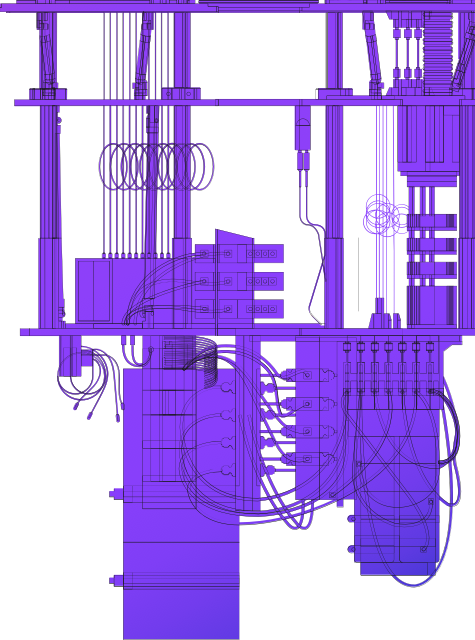
\includegraphics[width=\linewidth]{gfx/quantum_computer.png}
        \end{columns}
    \end{frame}

    \begin{frame}[focus]
        Domande?
    \end{frame}

    \appendix

    \begin{frame}{Fonti}
        \bibliography{bibliography.bib}
        \bibliographystyle{plain}

        \vspace{.2cm}

        Riferimenti completi su: \url{https://github.com/visika/Tesi}
    \end{frame}

    \begin{frame}{Immagini}
        \begin{itemize}
            \item Visage Technologies Face Tracking and Analysis, by Abyssus
            \item Tesla Model 3 Headlights in Dever, Photo by Vlad Tchompalov on Unsplash
            \item An example of a diseased cassava leaf. https://www.blog.google/technology/ai/ai-takes-root-helping-farmers-identity-diseased-plants/
        \end{itemize}
    \end{frame}

    \section{Quantum computing}

    \begin{frame}{Bit}
        \begin{columns}
            \column{0.3\textwidth}
            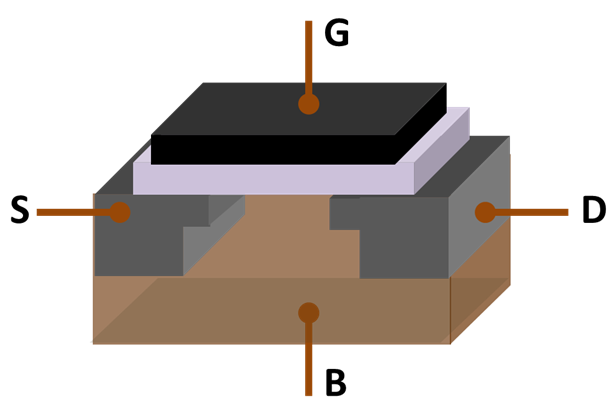
\includegraphics[width=\textwidth]{gfx/MOSFET_Structure.png}
            \column{0.7\textwidth}
            \begin{itemize}
                \item Solitamente implementati attraverso MOSFET\footnote{MOSFET: Metal Oxide Semiconductor Field Effect Transistor}
                \item 2 stati definiti: 0 e 1
                \item Può trovarsi in uno tra gli stati 0 o 1
            \end{itemize}
        \end{columns}
    \end{frame}

    \begin{frame}{Qubit}
        \begin{columns}
            \column{0.3\textwidth}
            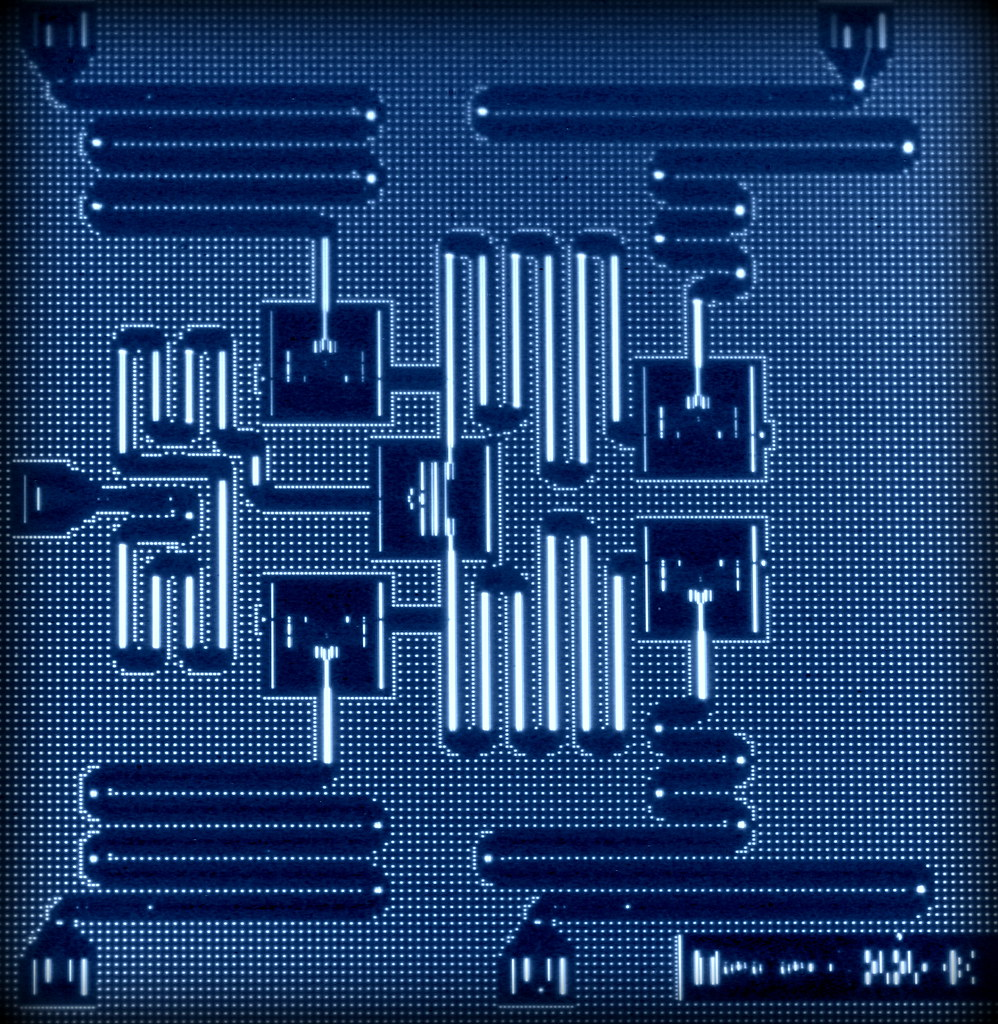
\includegraphics[width=\textwidth]{gfx/qubit}
            \column{0.7\textwidth}
            \begin{itemize}
                \item Implementato in diversi modi: giunzioni superconduttive, ioni intrappolati, fotoni polarizzati\ldots
                \item Due stati definiti: $\ket{0}$ e $\ket{1}$
                \item Può trovarsi in una sovrapposizione degli stati $\ket{0}$ e $\ket{1}$
            \end{itemize}
        \end{columns}
    \end{frame}

    \begin{frame}{Qubit}
        Matematicamente, la sovrapposizione di un qubit è espressa come
        \begin{equation*}
            \ket{\psi} = \alpha \ket{0} + \beta \ket{1} = \begin{matrix}
                0 \\ 1
            \end{matrix}\begin{pmatrix}
                \alpha \\ \beta
            \end{pmatrix}
            , \quad \alpha, \beta \in \mathbb{C}, 
        \end{equation*}
        dove $\alpha$ e $\beta$ sono chimate ampiezze di probabilità. 
        
        L'ultimo termine è chiamato vettore di probabilità. 
    \end{frame}

    \begin{frame}{Sfera di Bloch}
        \begin{columns}
            \column{.3\textwidth}
            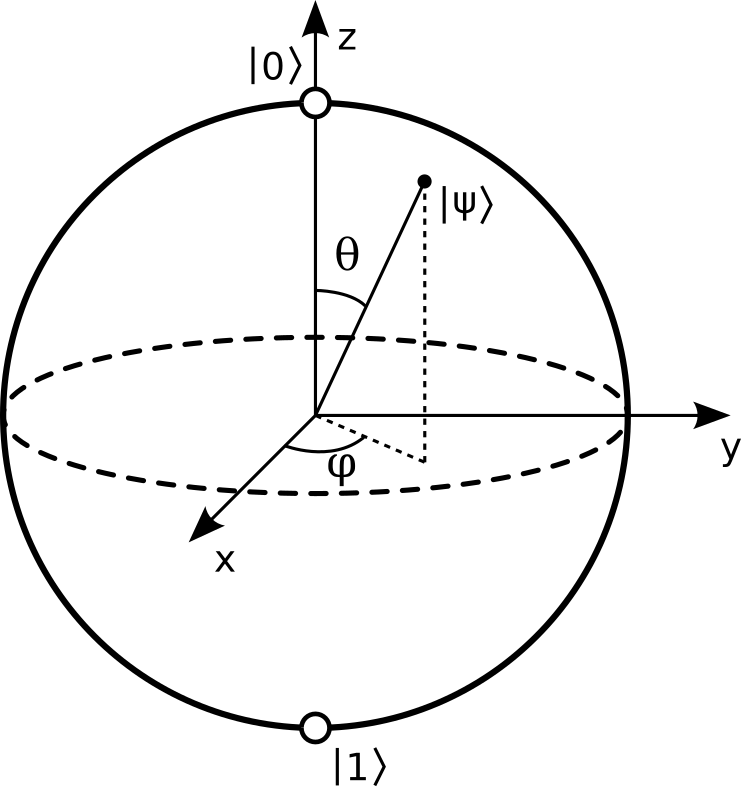
\includegraphics[width=\textwidth]{gfx/Bloch_sphere.png}
            \column{.7\textwidth}
            Un qubit si può visualizzare su una 2-sfera parametrizzando $\alpha$ e $\beta$ in coordinate polari
            \begin{equation*}
                \ket{\psi} = \cos \frac{\theta}{2} \ket{0} + e^{i\varphi}\sin \frac{\theta}{2} \ket{1},
            \end{equation*}
            dove $0\leq\theta\leq\pi$ e $0\leq\varphi<2\pi$
        \end{columns}
    \end{frame}

    \begin{frame}{Registro di 2 qubit}
        Un computer quantistico con $n$ qubit ha $2^n$ ampiezze di probabilità. 

        Lo stato di un registro a più qubit è rappresentato dal prodotto tensoriale dello stato dei singoli qubit. 

        \begin{equation*}
            \ket{00} = \ket{0} \otimes \ket{0}
        \end{equation*}
        \begin{equation*}
            \ket{\psi} = c_0 \ket{00} + c_1 \ket{01} + c_2 \ket{10} + c_3 \ket{11} = 
            \begin{matrix}
                00 \\ 01 \\ 10 \\ 11
            \end{matrix} \begin{pmatrix}
                c_0 \\ c_1 \\ c_2 \\ c_3
            \end{pmatrix}
        \end{equation*}
    \end{frame}

    \begin{frame}{Registro di $n$ qubit}
        Un computer quantistico con $n$ qubit ha $2^n$ ampiezze di probabilità. 

        Lo stato di un registro a più qubit è rappresentato dal prodotto tensoriale dello stato dei singoli qubit. 

        \begin{equation*}
            \ket{00\ldots00} = \ket{0} \otimes \ket{0} \otimes \ldots \otimes \ket{0} \otimes \ket{0}
        \end{equation*}
        \begin{equation*}
            \begin{split}
                \ket{\psi} &= c_0 \ket{00\ldots00} + c_1 \ket{00\ldots01} + \ldots + c_{n-2} \ket{11\ldots10} + \\ 
                &+ c_{n-1} \ket{11\ldots11} = \begin{matrix}
                00\ldots00 \\ 00\ldots01 \\ \vdots \\ 11\ldots10 \\ 11\ldots11
            \end{matrix} \begin{pmatrix}
                c_0 \\ c_1 \\ \vdots \\ c_{n-2} \\ c_{n-1}
            \end{pmatrix}
            \end{split}
        \end{equation*}
    \end{frame}

    \begin{frame}{Porte logiche quantistiche}
        Per manipolare $n$ qubit esistono apposite porte logiche quantistiche, 
        che sono operatori unitari rappresentabili come matrici $2^n\times2^n$. 
        
        \begin{columns}
            \column{.3\textwidth}
            \begin{center}
                Hadamard
            \end{center}
            \column{.3\textwidth}
            \begin{center}
                CNOT = CX
            \end{center}
            \column{.3\textwidth}
            \begin{center}
                Toffoli
            \end{center}
        \end{columns}

        \begin{columns}
            \column{.3\textwidth}
            \begin{figure}[h]
                \centering
                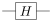
\includegraphics[width=\columnwidth]{gfx/Hadamard_gate}
                \label{fig:hadamard}
            \end{figure}
            \column{.3\linewidth}
            \begin{figure}[h]
                \centering
                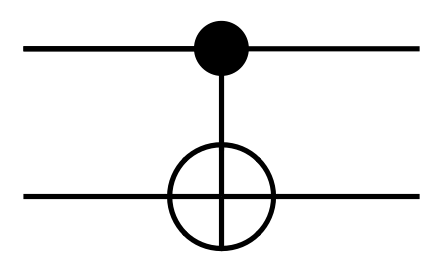
\includegraphics[width=\columnwidth]{gfx/CNOT_gate}                
                \label{fig:cnot}
            \end{figure}
            \column{.3\linewidth}
            \begin{figure}[h]
                \centering
                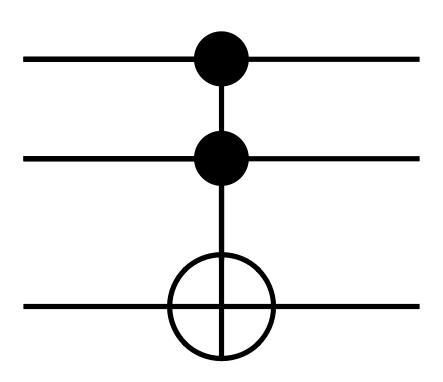
\includegraphics[width=\columnwidth]{gfx/Toffoli_gate}                
                \label{fig:toffoli}
            \end{figure}
        \end{columns}

        \vspace{-2em}

        \begin{columns}
            \column{.3\linewidth}
            \begin{equation*}
                \frac{1}{\sqrt{2}}
                \begin{pmatrix}
                    1 & 1 \\ 1 & -1
                \end{pmatrix}
            \end{equation*}
            \column{.3\linewidth}
            \begin{equation*}
                \begin{pmatrix}
                    1 & 0 & 0 & 0 \\
                    0 & 1 & 0 & 0 \\
                    0 & 0 & 0 & 1 \\
                    0 & 0 & 1 & 0
                \end{pmatrix}
            \end{equation*}
            \column{.3\linewidth}
            \begin{equation*}
                \begin{pmatrix}
                    \mathbb{I}_6 & 0 & 0 \\
                    0 & 0 & 1 \\
                    0 & 1 & 0
                \end{pmatrix}
            \end{equation*}
        \end{columns}
    \end{frame}

    \begin{frame}{Punti di forza dei quantum computer}
        \begin{columns}
            \column{.45\textwidth}
            \begin{tabular}{p{.15\textwidth}p{.8\textwidth}}
                \# di qubit & RAM classica richiesta \\ \hline
                5 & 256 byte \\ 
                25 & 2 gigabyte \\ 
                50 & 8000 terabyte \\ 
                275 & numero di atomi nell'universo osservabile 
            \end{tabular}
            \column{.45\textwidth}
            Le $n$ ampiezze di probabilità possono essere usate per memorizzare quantità enormi di informazioni. 

            Possiamo inoltre creare e lavorare su più copie in parallelo degli stessi dati. 
        \end{columns}
    \end{frame}

    \begin{frame}{Algoritmo per classificatore binario}
        \begin{block}{Inizializzazione dei registri quantistici}
            a = QuantumRegister(1, 'a') \\
            m = QuantumRegister(1, 'm') \\
            i = QuantumRegister(1, 'i') \\
            c = QuantumRegister(1, 'c') \\
            b = ClassicalRegister(2, 'bit') \\
            circuit = QuantumCircuit(a, m, i, c, b)
        \end{block}

        \begin{block}{Sovrapposizione degli stati}
            circuit.h(a) \\
            circuit.h(m)
        \end{block}

        \begin{block}{Codifica del vettore d'input}
            circuit.cry(x0, a[0], i[0]) \\
            circuit.x(a) \# entanglement dell'ancilla con 0
        \end{block}
    \end{frame}

    \begin{frame}{Algoritmo per classificatore binario}
        \begin{block}{Codifica dei vettori di training}
            circuit.mcry(t0, a[:] + m[:], i[0], None) \\
            circuit.x(m) \# entanglement di m con 0 \\
            circuit.mcry(t1, a[:] + m[:], i[0], None) \\
            circuit.cx(m, c) \# entanglement della classe 1 con m 1 \\
        \end{block}

        \begin{block}{Interferenza degli stati}
            circuit.h(a)
        \end{block}
        
        \begin{block}{Operazione di misura}
            circuit.measure(a, b[0]) \\
            circuit.measure(c, b[1]) \\
        \end{block}
        \# circuit.draw(output='mpl')
    \end{frame}

    \begin{frame}{Algoritmo per classificatore multiclasse}
        \begin{block}{Inizializzazione dei registri quantistici}
            a = QuantumRegister(1, 'a') \# knn ancilla \\
            m = QuantumRegister(2, 'm') \# training vector index \\
            i = QuantumRegister(2, 'i') \# feature index \\
            r = QuantumRegister(1, 'r') \# rotation qubit \\
            q = QuantumRegister(5, 'q') \# qram ancilla \\
            c = QuantumRegister(2, 'c') \# class \\
            b = ClassicalRegister(4, 'bit') \\
            circuit = QuantumCircuit(a, m, i, r, q, c, b)
        \end{block}

        \begin{block}{Sovrapposizione degli stati}
            circuit.h(a) \\
            circuit.h(m) \\
            circuit.h(i) \\
            circuit.h(c)
        \end{block}
    \end{frame}

    \begin{frame}{Algoritmo per classificatore multiclasse}
        \begin{block}{Codifica dei vettori}
            \# circuit.cry(theta, control, target) \\
            \# circuit.mcry(theta, controls, target, ancillae) \\

            \# >> Encode the input vector >> \\

            encodeVector(circuit, inputVirginica, i, a[:] + i[:], r[0], q) \\ 

            circuit.x(a) \# entanglement dell'ancilla con 0 \\

            \# >> Encode the training vectors >> \\

            buildTrainingState(trainingArray) \\
        \end{block}
        \begin{block}{Interferenza e misura}
            circuit.measure(r, b[0]) \\
            circuit.h(a) \\
            circuit.measure(a, b[1]) \\
            circuit.measure(c[0], b[2]) \\
            circuit.measure(c[1], b[3])
        \end{block}
    \end{frame}

    \begin{frame}{Algoritmo per classificatore multiclasse}
        \begin{block}{Definizione dei costruttori}
            def encodeTraining(circuit, data, i, controls, rotationQ, ancillaQ, c, m): \\
            \# Header \\
            encodeClass(circuit, c) \\
            encodeIndex(circuit, m) \\
            \# Encoder \\
            encodeVector(circuit, data, i, controls, rotationQ, ancillaQ) \\
            \# Footer \\
            encodeClass(circuit, c) \\
            encodeIndex(circuit, m)
        \end{block}
    \end{frame}

    \begin{frame}{Algoritmo per classificatore multiclasse}
        \begin{block}{Definizione del codificatore}
            def encodeVector(circ, data, i, controls, rotationQ, ancillaQ): \\
            \# |00>\\
            circuit.x(i)\\
            circuit.mcry(data[0], controls, rotationQ, ancillaQ)\\
            circuit.x(i)\\
            \# |01>\\
            circuit.x(i[1])\\
            circuit.mcry(data[1], controls, rotationQ, ancillaQ)\\
            circuit.x(i[1])\\
            \# |10>\\
            circuit.x(i[0])\\
            circuit.mcry(data[2], controls, rotationQ, ancillaQ)\\
            circuit.x(i[0])\\
            \# |11>\\
            circuit.mcry(data[3], controls, rotationQ, ancillaQ)
        \end{block}
    \end{frame}

    \begin{frame}{Routine FF-QRAM}
        \begin{equation*}
            \ket{\psi_0}_l = \psi_{\vec{d}^{(l)}} \ket{\vec{d}^{(l)}} \ket{0}_R + \sum_{j \neq \vec{d}^{(l)}} \psi_j \ket{j} \ket{0}_R
        \end{equation*}

        \begin{equation*}
            \ket{\psi_1}_l = \psi_{\vec{d}^{(l)}} \ket{1}^{\otimes n} \ket{0}_R + \sum_{\ket{\overline{j \oplus \vec{d}^{(l)}}} \neq \ket{1}^{\otimes n}} \psi_j \overline{j \oplus \vec{d}^{(l)}} \ket{0}_R
        \end{equation*}

        \begin{equation*}
            \ket{\psi_2}_l = \psi_{\vec{d}^{(l)}} \ket{1}^{\otimes n} \ket{\theta^{(l)}}_R + \sum_{\ket{\overline{j \oplus \vec{d}^{(l)}}} \neq \ket{1}^{\otimes n}} \psi_j \ket{\overline{j \oplus \vec{d}^{(l)}}} \ket{0}_R
        \end{equation*}
        
        \begin{equation*}
            \ket{\psi_3}_l = \psi_{\vec{d}^{(l)}} \ket{\vec{d}^{(l)}} \ket{\theta}_R + \sum_{j \neq \vec{d}^{(l)}} \psi_j \ket{j} \ket{0}_R
        \end{equation*}

        \begin{equation*}
            \ket{\psi_4}_{l,l+1} = \psi_{\vec{d}^{(l)}} \ket{\vec{d}^{(l)}} \ket{\theta^{(l)}}_R + \psi_{\vec{d}^{(l+1)}} \ket{\vec{d}^{(l+1)}} \ket{\theta^{(l+1)}}_R + \sum_{j \neq \vec{d}^{(l)},\vec{d}^{(l+1)}} \psi_j \ket{j} \ket{0}_R
        \end{equation*}
    \end{frame}

    \begin{frame}{Routine FF-QRAM}
        \begin{equation*}
            \sum_{l=0}^{M-1} \psi_{\vec{d}^{(l)}} \ket{\vec{d}^{(l)}} \left[ \cos\theta^{(l)} \ket{0}_R + \sin\theta^{(l)} \ket{1}_R \right] + \sum_{j \notin \{ \vec{d}^{(l)} \}} \psi_j \ket{j} \ket{0}_R
        \end{equation*}

        \begin{equation*}
            \text{P}(1) = \sum_{l=0}^{M-1} | \psi_{\vec{d}^{(l)}} \sin\theta^{(l)} |^2
        \end{equation*}
    \end{frame}

    \begin{frame}{QRAM per QSVM}
        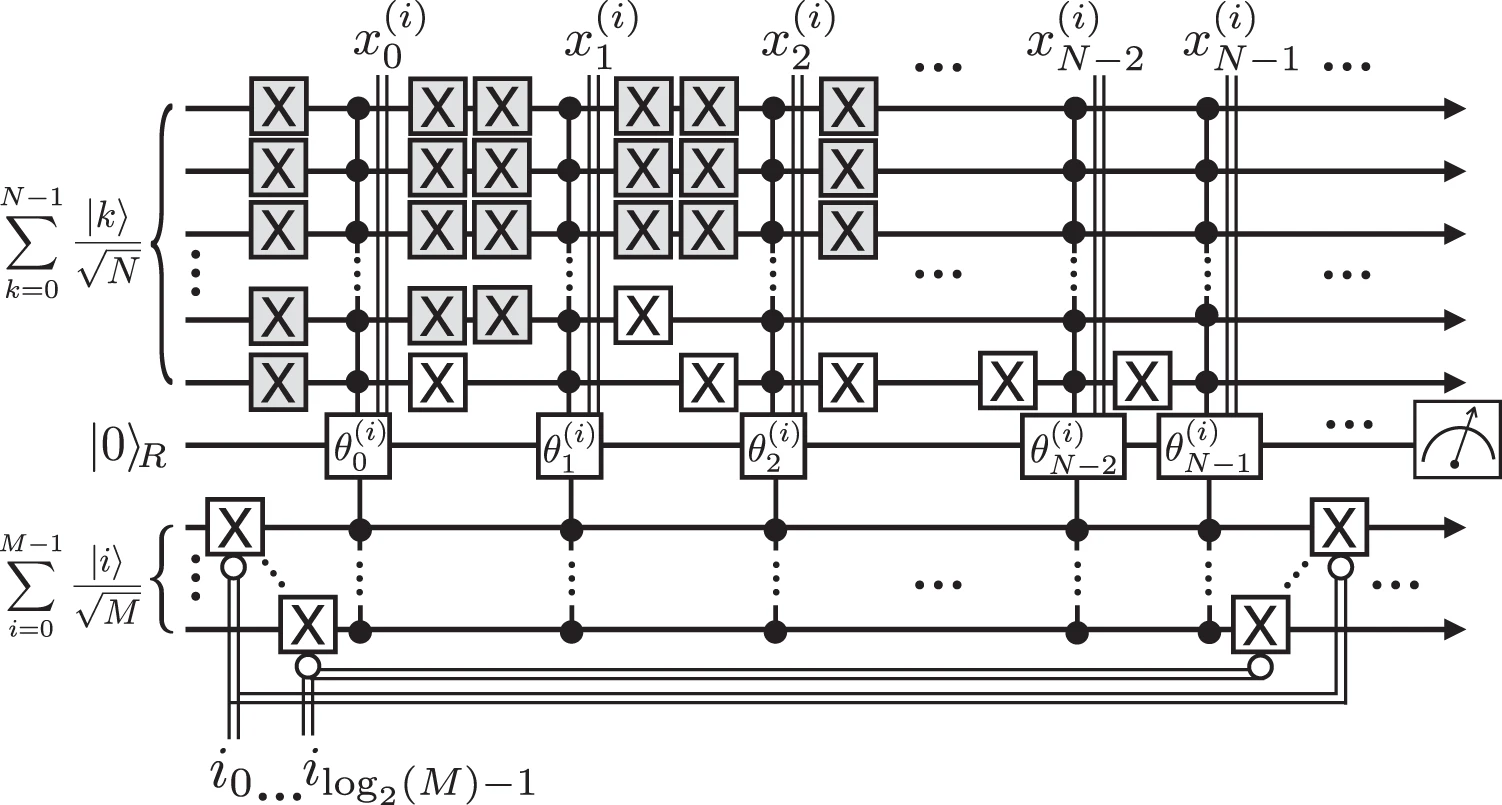
\includegraphics[width=\linewidth]{gfx/qram_qsvm.png}
    \end{frame}

\end{document}
